% ******************************* PhD Thesis Template **************************
% Please have a look at the README.md file for info on how to use the template

\documentclass[a4paper,12pt,customfont,numbered,print,custommargin,oneside]{Classes/PhDThesisPSnPDF}

% ******************************************************************************
% ******************************* Class Options ********************************
% *********************** See README for more details **************************
% ******************************************************************************

% `a4paper'(The University of Cambridge PhD thesis guidelines recommends a page
% size a4 - default option) or `a5paper': A5 Paper size is also allowed as per
% the Cambridge University Engineering Deparment guidelines for PhD thesis
%
% `11pt' or `12pt'(default): Font Size 10pt is NOT recommended by the University
% guidelines
%
% `oneside' or `twoside'(default): Printing double side (twoside) or single
% side.
%
% `print': Use `print' for print version with appropriate margins and page
% layout. Leaving the options field blank will activate Online version.
%
% `index': For index at the end of the thesis
%
% `draftclassic': For draft mode without loading any images (same as draft in book)
%
% `draft': Special draft mode with line numbers, images, and water mark with
% timestamp and custom text. Position of the text can also be modified.
%
% `abstract': To generate only the title page and abstract page with
% dissertation title and name, to submit to the Student Registry
%
% `chapter`: This option enables only the specified chapter and it's references
%  Useful for review and corrections.
%
% ************************* Custom Page Margins ********************************
%
% `custommargin`: Use `custommargin' in options to activate custom page margins,
% which can be defined in the preamble.tex. Custom margin will override
% print/online margin setup.
%
% *********************** Choosing the Fonts in Class Options ******************
%
% `times' : Times font with math support. (The Cambridge University guidelines
% recommend using times)
%
% `fourier': Utopia Font with Fourier Math font (Font has to be installed)
%            It's a free font.
%
% `customfont': Use `customfont' option in the document class and load the
% package in the preamble.tex
%
% default or leave empty: `Latin Modern' font will be loaded.
%
% ********************** Choosing the Bibliography style ***********************
%
% `authoryear': For author-year citation eg., Krishna (2013)
%
% `numbered': (Default Option) For numbered and sorted citation e.g., [1,5,2]
%
% `custombib': Define your own bibliography style in the `preamble.tex' file.
%              `\RequirePackage[square, sort, numbers, authoryear]{natbib}'.
%              This can be also used to load biblatex instead of natbib
%              (See Preamble)
%
% **************************** Choosing the Page Style *************************
%
% `default (leave empty)': For Page Numbers in Header (Left Even, Right Odd) and
% Chapter Name in Header (Right Even) and Section Name (Left Odd). Blank Footer.
%
% `PageStyleI': Chapter Name next & Page Number on Even Side (Left Even).
% Section Name & Page Number in Header on Odd Side (Right Odd). Footer is empty.
%
% `PageStyleII': Chapter Name on Even Side (Left Even) in Header. Section Number
% and Section Name in Header on Odd Side (Right Odd). Page numbering in footer


% ********************************** Preamble **********************************
% Preamble: Contains packages and user-defined commands and settings
% ******************************************************************************
% ****************************** Custom Margin *********************************

% Add `custommargin' in the document class options to use this section
% Set {innerside margin / outerside margin / topmargin / bottom margin}  and
% other page dimensions
\ifsetCustomMargin
  \RequirePackage[left=37mm,right=30mm,top=35mm,bottom=30mm]{geometry}
  \setFancyHdr % To apply fancy header after geometry package is loaded
\fi

% Add spaces between paragraphs
%\setlength{\parskip}{0.5em}
% Ragged bottom avoids extra whitespaces between paragraphs
\raggedbottom
% To remove the excess top spacing for enumeration, list and description.
% Phong: actually for me, spacing among items is too much.
\usepackage{enumitem}
\setlist[enumerate,itemize,description]{itemsep=0em}

% *****************************************************************************
% ******************* Fonts (like different typewriter fonts etc.)*************

% Add `customfont' in the document class option to use this section

\ifsetCustomFont
  % Set your custom font here and use `customfont' in options. Leave empty to
  % load computer modern font (default LaTeX font).
  %\RequirePackage{helvet}

  % For use with XeLaTeX
  %  \setmainfont[
  %    Path              = ./libertine/opentype/,
  %    Extension         = .otf,
  %    UprightFont = LinLibertine_R,
  %    BoldFont = LinLibertine_RZ, % Linux Libertine O Regular Semibold
  %    ItalicFont = LinLibertine_RI,
  %    BoldItalicFont = LinLibertine_RZI, % Linux Libertine O Regular Semibold Italic
  %  ]
  %  {libertine}
  %  % load font from system font
  %  \newfontfamily\libertinesystemfont{Linux Libertine O}
  
\usepackage{mathpazo}
\renewcommand*\rmdefault{ppl}
\renewcommand*\sfdefault{phv}
\renewcommand*\ttdefault{lmtt}

\fi

% *****************************************************************************
% **************************** Custom Packages ********************************

% ************************* Algorithms and Pseudocode **************************

%\usepackage{algpseudocode}


% ********************Captions and Hyperreferencing / URL **********************

% Captions: This makes captions of figures use a boldfaced small font.
\RequirePackage[bf,font={small,sf}]{caption}
\usepackage{url}
\urlstyle{tt}

% *************************** Graphics and figures *****************************

% Allow XeLatex to include images without specifying extension
\DeclareGraphicsExtensions{.pdf,.png,.jpg}

%\usepackage{rotating}
%\usepackage{wrapfig}

% Uncomment the following two lines to force Latex to place the figure.
% Use [H] when including graphics. Note 'H' instead of 'h'
%\usepackage{float}
%\restylefloat{figure}

% Subcaption package is also available in the sty folder you can use that by
% uncommenting the following line
% This is for people stuck with older versions of texlive
%\usepackage{sty/caption/subcaption}
\usepackage{subcaption}


% ********************************** Tables ************************************
\usepackage{booktabs} % For professional looking tables
\usepackage{multirow}
\setlength{\tabcolsep}{8pt} % a bit more space between columns

%\usepackage{multicol}
%\usepackage{longtable}
\usepackage{tabularx}
\newcolumntype{L}[1]{>{\raggedright\arraybackslash}p{#1}}
\newcolumntype{C}[1]{>{\centering\arraybackslash}p{#1}}
\newcolumntype{R}[1]{>{\raggedleft\arraybackslash}p{#1}}
\newcolumntype{Y}{>{\raggedright\arraybackslash}X}

% *********************************** SI Units *********************************
\usepackage{siunitx} % use this package module for SI units


% ******************************* Line Spacing *********************************

% Choose linespacing as appropriate. Default is one-half line spacing as per the
% University guidelines

% \doublespacing
% \onehalfspacing
% \singlespacing


% ************************ Formatting / Footnote *******************************

% Don't break enumeration (etc.) across pages in an ugly manner (default 10000)
%\clubpenalty=500
%\widowpenalty=500

%\usepackage[perpage]{footmisc} %Range of footnote options


% *****************************************************************************
% *************************** Bibliography  and References ********************

%\usepackage{cleveref} %Referencing without need to explicitly state fig /table

% Add `custombib' in the document class option to use this section
\ifuseCustomBib
   \RequirePackage[square, sort, numbers, authoryear]{natbib} % CustomBib

% If you would like to use biblatex for your reference management, as opposed to the default `natbibpackage` pass the option `custombib` in the document class. Comment out the previous line to make sure you don't load the natbib package. Uncomment the following lines and specify the location of references.bib file

%\RequirePackage[backend=biber, style=numeric-comp, citestyle=numeric, sorting=nty, natbib=true]{biblatex}
%\bibliography{References/references} %Location of references.bib only for biblatex

\fi

% changes the default name `Bibliography` -> `References'
\renewcommand{\bibname}{References}

% ******************************** Roman Pages *********************************
% The romanpages environment set the page numbering to lowercase roman one
% for the contents and figures lists. It also resets
% page-numbering for the remainder of the dissertation (arabic, starting at 1).

\newenvironment{romanpages}{
  \setcounter{page}{1}
  \renewcommand{\thepage}{\roman{page}}}
{\newpage\renewcommand{\thepage}{\arabic{page}}}


% ******************************************************************************
% ************************* User Defined Commands ******************************
% ******************************************************************************

% *********** To change the name of Table of Contents / LOF and LOT ************

\renewcommand{\contentsname}{Contents}
%\renewcommand{\listfigurename}{My List of Figures}
%\renewcommand{\listtablename}{My List of Tables}


% ********************** TOC depth and numbering depth *************************

\setcounter{secnumdepth}{3}
\setcounter{tocdepth}{3}


% ******************************* Nomenclature *********************************

% To change the name of the Nomenclature section, uncomment the following line

%\renewcommand{\nomname}{Symbols}


% ********************************* Appendix ***********************************

% The default value of both \appendixtocname and \appendixpagename is `Appendices'. These names can all be changed via:

%\renewcommand{\appendixtocname}{List of appendices}
%\renewcommand{\appendixname}{Appndx}

% *********************** Configure Draft Mode **********************************

% Uncomment to disable figures in `draftmode'
%\setkeys{Gin}{draft=true}  % set draft to false to enable figures in `draft'

% These options are active only during the draft mode
% Default text is "Draft"
%\SetDraftText{DRAFT}

% Default Watermark location is top. Location (top/bottom)
%\SetDraftWMPosition{bottom}

% Draft Version - default is v1.0
%\SetDraftVersion{v1.1}

% Draft Text grayscale value (should be between 0-black and 1-white)
% Default value is 0.75
%\SetDraftGrayScale{0.8}


% ******************************** Todo Notes **********************************
%% Uncomment the following lines to have todonotes.

%\ifsetDraftClassic
%	\usepackage[colorinlistoftodos]{todonotes}
%	\newcommand{\mynote}[1]{\todo[author=kks32,size=\small,inline,color=green!40]{#1}}
%\else
%	\newcommand{\mynote}[1]{}
%	\newcommand{\listoftodos}{}
%\fi

% Example todo: \mynote{Hey! I have a note}

% Use this package to annotate on specific text
\usepackage[inline]{Sty/trackchanges}

% Always include todo notes
\usepackage[colorinlistoftodos]{todonotes}
\presetkeys{todonotes}{size=\scriptsize\sffamily}{}
\newcommand{\issue}[1]{\todo[inline,color=red!50]{#1}}


% ******************************** Phong's additional changes **********************************
% Format headings
\usepackage{titlesec}  

%\titleformat{\chapter}[display]
%	{\filcenter}
%	{\color{Gray}\Huge Chapter \thechapter}{0pt}
%	{\color{NavyBlue}\Huge\sffamily}
\titleformat{\section}{\sffamily\Large\color{NavyBlue}}{\thesection}{16pt}{}
\titleformat{\subsection}{\sffamily\large\color{NavyBlue}}{\thesubsection}{14pt}{}
\titleformat{\subsubsection}{\sffamily\color{NavyBlue}}{\thesubsubsection}{12pt}{}
\titleformat{\paragraph}[runin]{\sffamily\bfseries\color{NavyBlue}}{\theparagraph}{}{}
\titleformat{\subparagraph}[runin]{\sffamily\itshape\color{NavyBlue}}{\thesubparagraph}{}{}

% fancy chapter
\definecolor{chapbgcolor}{HTML}{DFEDFF}
\definecolor{chapnumcolor}{HTML}{7FB7FF}

\usepackage[Bjornstrup]{fncychap}
\ChNumVar{\fontsize{76}{80}\usefont{T1}{phv}{m}{n}\selectfont}
\ChTitleVar{\raggedleft\color{NavyBlue}\Huge\sffamily}

\makeatletter

\renewcommand\DOCH{%
	\settowidth{\py}{\CNoV\thechapter}
	\addtolength{\py}{-10pt}
	\fboxsep=0pt%
	\colorbox{chapbgcolor}{\rule{0pt}{40pt}\parbox[b]{\textwidth}{\hfill}}%
	\kern-\py\raise20pt%
	\hbox{\color{chapnumcolor}\CNoV\thechapter}\\%
}

\renewcommand\DOTI[1]{%
	\nointerlineskip\raggedright%
	\fboxsep=\myhi%
	\vskip-1ex%
	\colorbox{chapbgcolor}{\parbox[t]{\mylen}{\CTV\FmTi{#1}}}\par\nobreak%
	\vskip 40pt%
}

\renewcommand\DOTIS[1]{%
	\fboxsep=0pt
	\colorbox{chapbgcolor}{\rule{0pt}{40pt}\parbox[b]{\textwidth}{\hfill}}\\%
	\nointerlineskip\raggedright%
	\fboxsep=\myhi%
	\colorbox{chapbgcolor}{\parbox[t]{\mylen}{\CTV\FmTi{#1}}}\par\nobreak%
	\vskip 40pt%
}
\makeatother

% Improve verbatim
\usepackage{listings}
\lstset{
	columns=flexible,
	breaklines=true
}

% continued numbered list
\newcounter{listnum}

% Emphasized text
\newcommand{\strong}[1]{{\textbf{\color{NavyBlue}{#1}}}} 

% check and cross
\usepackage{amssymb}% http://ctan.org/pkg/amssymb
\usepackage{pifont}% http://ctan.org/pkg/pifont
\newcommand{\cmark}{\ding{51}}%
\newcommand{\xmark}{\ding{55}}%

% for the TimeSets citation figure
\definecolor{f2}{HTML}{51A7F9}
\newcommand{\tshierarchy}{\colorbox[HTML]{8dd3c7}{\emph{hierarchy}}}
\newcommand{\tsinteraction}{\colorbox[HTML]{bebada}{\emph{interaction}}}
\newcommand{\tsoverview}{\colorbox[HTML]{FDB462}{\emph{overview}}}
\newcommand{\tsnetwork}{\colorbox[HTML]{FCCDE5}{\emph{network}}}
\newcommand{\tsgraph}{\colorbox[HTML]{80b1d3}{\emph{graph}}}
\newcommand{\tsclustering}{\colorbox[HTML]{B3DE69}{\emph{clustering}}}
\newcommand{\tsevaluation}{\colorbox[HTML]{FFFFb3}{\emph{evaluation}}}

% Image source
\newcommand{\is}[1]{{\textrm{\emph{Image source:~#1}}}} 


% ************************ Thesis Information & Meta-data **********************
% Thesis title and author information, refernce file for biblatex
% ************************ Thesis Information & Meta-data **********************
%% The title of the thesis
\title{
	Supporting the Sensemaking Process: An Analytic Provenance Approach\\?or?\\
	Provenance Data Visualization \\for Support Sensemaking
	}

%\texorpdfstring is used for PDF metadata. Usage:
%\texorpdfstring{LaTeX_Version}{PDF Version (non-latex)} eg.,
%\texorpdfstring{$sigma$}{sigma}

%% Subtitle (Optional)
%\subtitle{Using the CUED template}

%% The full name of the author
\author{Phong H. Nguyen}

%% Department (eg. Department of Engineering, Maths, Physics)
\dept{School of Science and Technology}

%% University and Crest
\university{Middlesex University}
% Crest minimum should be 30mm.
\crest{
\includegraphics[width=0.25\textwidth]{MdxShield}}
%% Use this crest, if you are using the college crest
%% Crest long miminum should be 65mm
%\crest{\includegraphics[width=0.45\textwidth]{University_Crest_Long}}

%% College shield [optional] 
% Crest minimum should be 30mm.
%\collegeshield{\includegraphics[width=0.2\textwidth]{CollegeShields/Kings}}


%% Supervisor (optional)
\supervisor{Associate Professor Kai Xu}
%% Supervisor Role (optional) - Supervisor (default) or advisor
\supervisorrole{}
\advisor{Professor William Wong}
\advisorrole{}
%% Advisor (optional)
%\advisor{Prof. William Wong}
%%% Advisor Role (optional) - Advisor (default) or leave empty
%\advisorrole{Supervisor: }


%% You can redefine the submission text:
% Default as per the University guidelines:
% ``This dissertation is submitted for the degree of''
%\renewcommand{\submissiontext}{change the default text here if needed}

%% Full title of the Degree
\degreetitle{Doctor of Philosophy}

%% College affiliation (optional)
%\college{London}

%% Submission date
% Default is set as {\monthname[\the\month]\space\the\year}
%\degreedate{September 2014} 

%% Meta information
%\subject{LaTeX} \keywords{{LaTeX} {PhD Thesis} {Engineering} {University of Cambridge}}
\subject{PhD Thesis} \keywords{{Sensemaking} {Analytic Provenance} {Information Visualization}}

% ***************************** Abstract Separate ******************************
% To printout only the titlepage and the abstract with the PhD title and the
% author name for submission to the Student Registry, use the `abstract' option in
% the document class.

\ifdefineAbstract
 \pagestyle{empty}
 \includeonly{Declaration/declaration, Abstract/abstract}
\fi

% ***************************** Chapter Mode ***********************************
% The chapter mode allows user to only print particular chapters with references
% Title, Contents, Frontmatter are disabled by default
% Useful option to review a particular chapter or to send it to supervisior.
% To use choose `chapter' option in the document class

\ifdefineChapter
\includeonly{Chapter1/chapter1}
\fi

% ******************************** Front Matter ********************************
\begin{document}

\frontmatter

\begin{titlepage}
%  \maketitle
\end{titlepage}


%% ******************************* Thesis Dedidcation ********************************

\begin{dedication} 

For my wife, \\Hien Nguyen.

\end{dedication}


%% ******************************* Thesis Declaration ***************************

\begin{declaration}

I hereby declare that except where specific reference is made to the work of 
others, the contents of this dissertation are original and have not been 
submitted in whole or in part for consideration for any other degree or 
qualification in this, or any other university. This dissertation is my own 
work and contains nothing which is the outcome of work done in collaboration 
with others, except as specified in the text and Acknowledgements. This 
dissertation contains fewer than 65,000 words including appendices, 
bibliography, footnotes, tables and equations and has fewer than 150 figures.

% Author and date will be inserted automatically from thesis.tex \author \degreedate

\end{declaration}


%% ************************** Thesis Acknowledgements **************************

\begin{acknowledgements}      
\lettrine{F}{irst} and foremost, I would like to express my deep and sincere gratitude to my supervisor, Associate Professor Kai Xu, for his warm encouragement and thoughtful guidance. He has always extended his time in crucial stages of my PhD journey. I still remember how crazy my first submission to the IEEE VAST conference was. On $31^{st}$ March, 2013 -- the submission deadline and Easter Sunday by the way -- Kai and I went to the library to work on the paper. We had Vietnamese food for lunch and pizza for dinner, and had to leave the library at midnight because of the holiday. We went to his house and continued working and submitting until the deadline passed at 1am. Then, he drove me home. What else can I ask for from a supervisor? Even though the submission was rejected, the knowledge and experience I learned from him helped me become a better researcher. As a result, at the third and fourth attempts, I published two VAST papers now.

I am indebted to my second supervisor, Professor William Wong, for his valuable advice. As the head of the Interaction Design Center and the principal investigator of an 18-partner EU-funded project, he is extremely busy. However, William always finds time to discuss about my PhD and encourage me to think deeply about the big picture of my work. I also would like to thank him for his financial support through part-time projects and his annual barbecue events. He is a good chief.

I am grateful to Dr Peter Passmore who was the examiner in my Registration and Transfer vivas for his questions and feedback on my work. I would like to thank my colleagues Dr Neesha Kodagoda, Dr Chris Rooney, Dr Rick Walker, Dr Yongjun Zheng, Dr Simon Attfield, Dr Bob Fields, Ashley Wheat and Dr Nallini Selvaraj for their lively discussion, joy and fun in doing research together in the center. I would like to thank Dr Dong-Han Ham, Dr Aidan Slingsby, Dr Jason Dykes, Dr Jo Wood, Dr Derek Stephens, Dr T.J. Jankun-Kelly, Dr Andy Bardill,  Betul Salman and Dr Kate Herd with whom I had a privilege to collaborate in writing papers and to learn from them. I would like to thank all the PhD students that I see everyday, work and play together: Arni, Amar, Pragya, Joshua, Khrisna, Unai, Ali, Ran and many others that I might forget to mention.

I would like to acknowledge Middlesex University, particularly in the award of the research studentship that financially supported me doing this PhD. I would like to thank Professor Balbir Barn, the Deputy Dean of the Faculty of Science and Technology, who waived the tuition fee for my extra writing year.

Last but not least, I would like to give my special thanks to my parents and my small family: my wife Hien, my two daughters -- Lily and Bella. Their patience and love encouraged me to complete this work. To them I dedicate this thesis.

\end{acknowledgements}

%% ************************** Thesis Abstract *****************************
% Use `abstract' as an option in the document class to print only the titlepage and the abstract.
\begin{abstract}
\vspace{-0.7in}
\lettrine{S}{ensemaking} is an iterative and dynamic process, in which people collect data relevant to their tasks, analyze the collected information to produce new knowledge, and possibly inform further actions. During the sensemaking process, it is difficult for the human's working memory to keep track of the progress and to synthesize a large number of individual findings and derived hypotheses, thus limits the performance. \emph{Analytic provenance} captures both the data exploration process and and its accompanied reasoning, potentially addresses these information overload and disorientation problems. \emph{Visualization} can help recall, revisit and reproduce the sensemaking process through visual representations of provenance data. More interesting and challenging, analytic provenance has the potential to facilitate the ongoing sensemaking process rather than providing only post hoc support.

This thesis addresses the challenge of how to design interactive visualizations of analytic provenance data to support such an iterative and dynamic sensemaking. Its original contribution includes four visualizations that help users explore complex temporal and reasoning relationships hidden in the sensemaking problems, using both automatically and manually captured provenance. First \emph{SchemaLine}, a timeline visualization, enables users to construct and refine narratives from their annotations. Second, \emph{TimeSets} extends SchemaLine to explore more complex relationships by visualizing both temporal and categorical information simultaneously. Third, \emph{SensePath} captures and visualizes user actions to enable analysts to gain a deep understanding of the user's sensemaking process. Fourth, \emph{SenseMap} visualization prevents users from getting lost, synthesizes new relationship from captured information, and consolidates their understanding of the sensemaking problem. All of these four visualizations are developed using a user-centered design approach and evaluated empirically to explore how they help target users make sense of their real tasks. In summary, this thesis contributes novel and validated interactive visualizations of analytic provenance data that enable users to perform effective sensemaking.
\end{abstract}

% *********************** Adding TOC and List of Figures ***********************
%\tableofcontents

%\listoffigures
%
%\listoftables

% \printnomenclature[space] space can be set as 2em between symbol and description
%\printnomenclature[3em]
%\printnomenclature


% ******************************** Main Matter *********************************
\mainmatter


%%\begin{figure}[ht]
%	\centering
%	\includegraphics[width=\linewidth]{schemaline-layout-overview}
%\end{figure}

\begin{figure}[ht]
	\centering
	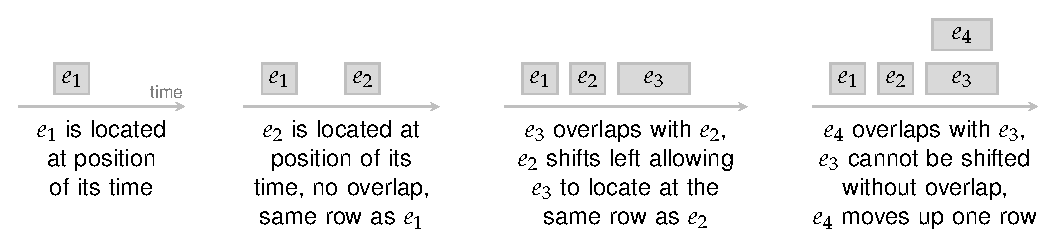
\includegraphics[width=\linewidth]{Chapter3/figures/layout-example}
\end{figure}

%\begin{figure}[ht]
%	\centering
%	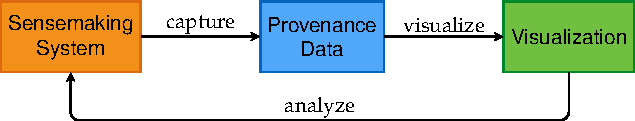
\includegraphics[width=.8\linewidth]{workflow}
%\end{figure}
%
%\begin{figure}[ht]
%	\centering
%	\includegraphics[width=.8\linewidth]{sensemap-views}
%\end{figure}
%\chapter{Introduction}
\label{chap:intro}

\graphicspath{{Chapter1/figures/}}

\emph{Sensemaking} reflects how we make sense of the world so that we can take further actions in it~\cite{Snowden2005}. More specifically, sensemaking is described as a motivated and continuous effort to understand the relationships among people, places and events around us in order to act more effectively~\cite{Klein2006a}. It is the process of collecting, representing and organizing complex information sets based on a particular problem we are solving in such a way that can help us understand the problem better and make sense of it~\cite{Russell2008}. For example, intelligence analysts may need to examine thousands of reports to establish deep understanding of particular persons or organizations before identifying possible threats from them. In a more ordinary and everyday context such as selecting a smartwatch, a person may search for different models on the Internet, learn unfamiliar technical terminologies, and consider pros and cons between those identified models. To effectively make sense of the problem, people need to digest a large amount of data: a few tens of smartwach models, a few thousands of documents, or a much bigger scale. The data around the world has been produced more rapidly than ever before, with major sources including sensors, machine logs, public websites and social media. For a single day, 50 million photos are uploaded on Instagram, 500 million tweets are sent on Twitter, 3.5 billion searches are performed on Google and 200 billion emails are sent~\footnote{\url{http://www.internetlivestats.com/}}. This data deluge could help us find more relevant information to our problems; however, it also poses a huge challenge in making sense of such a vast amount of data.

\emph{Visualization} can help people solve problems more effectively through visual representations of datasets~\cite{Munzner2014}. They can display a large amount of data in a way that quickly reveals hidden patterns. Interaction allows people to further investigate the visualized data in more detail and explore the relationship between identified patterns. Automated techniques in information retrieval and data mining can help speed up the sensemaking process. For instance, named-entity recognition techniques~\cite{Nadeau2007} can automatically identify entities from text and classify them into predefined categories such as persons, organizations and locations. This automation saves analysts a considerable amount of time in their common tasks such as findings all reports mentioning a particular person. \emph{Visual analytics} combines such automated analysis techniques and interactive visualizations to effectively make sense of very large and complex datasets~\cite{Keim2010}.

Research in visual analytics focuses on helping people reveal hidden patterns in the data; however, sensemaking requires support beyond that. Analysts may connect individual patterns to explore the relationships between them, generate potential hypotheses explaining those relationships, and find ways to verify them. Unfortunately, people with limited capacity of working memory cannot hold all of these artifacts simultaneously. They may forget previous findings and relations between them, or remember but fail to retrieve the information needed. They may also forget how those findings were derived, making it more difficult to find similar information. Especially for long and interrupted analysis sessions with big datasets, people often get lost in the problem space: they are unable to examine their progresses, unable to synthesize their discoveries, and unable to decide the next step effectively.

\emph{Analytic provenance} has the potential to address these problems. It is a subfield of  visual analytics, focusing on understanding a user's reasoning process through the study of their interactions with the computer system that supports sensemaking~\cite{North2011}. Analytic provenance captures both the interactive data exploration process and the accompanied reasoning process during sensemaking~\cite{Xu2015}, releasing analysts from a burden of keeping track of their discoveries. Analytic provenance data can be categorized using a multiple semantic layer model~\cite{Gotz2009}. Low-level provenance can be captured automatically but contains little semantics. Higher level provenance contains richer semantics, thus could be more useful in sensemaking. However, it is much more challenging to capture and primarily has to be done manually. Visualizations of provenance data have been developed for different purposes including recall, replication, action recovery, collaborative communication, presentation and meta-analysis~\cite{Ragan2016}. Most of these visualizations provide post hoc applications of provenance or stop at recalling the process and revisiting past steps. They are not specifically designed to support the ongoing, iterative and dynamic sensemaking process.

\section{Research Problem and Approach}

The central research problem of this thesis is
\begin{center}
	\strong{How to design interactive visualizations of analytic provenance data \\for supporting sensemaking?}
\end{center}

To approach the research problem, we propose a cyclic process model, in which analytic provenance can be used to support sensemaking as illustrated in \autoref{fig:intro-workflow}. The process starts with a \emph{user} employing a \emph{sensemaking system} to solve a problem. The sensemaking system could be any computer-based applications, such as a simple visualization tool, a complex visual analytics system and a standard web browser. During the sensemaking process, both the performed low-level actions (e.g., visualization interaction such as sort, filter and zoom) and the produced high-level reasoning artifacts (e.g., findings, assumptions and hypotheses) are captured. They are referred as \emph{provenance data} in the figure. Then, this provenance data should be visualized in a way that can provide support back to the ongoing sensemaking process. In this model, the user can interact with both the sensemaking system and the \emph{provenance visualization} to solve his or her problem. The provenance visualization should be able to communicate with the sensemaking system to facilitate the interplay between the user and these two. Technically, it can be implemented directly in the sensemaking system or separately as a provenance-enabled plug-in.

\begin{figure}[!htb]
	\centering
	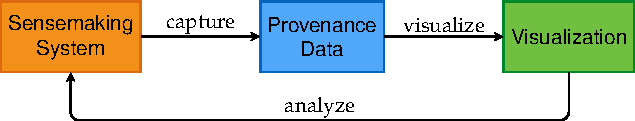
\includegraphics{workflow}
	\caption{A cyclic process model of supporting sensemaking through analytic provenance. While using a sensemaking system to solve a problem, the interaction and reasoning performed by the user are \emph{captured} and \emph{visualized} to provide \emph{support} back to the sensemaking process. The sensemaking system can be any computer-based applications such as visual analytics systems and web browsers. The two-way dash arrow indicates the communication between the provenance visualization and the sensemaking system to provide sensemaking support. As a result, the user can interact with both the sensemaking system and the provenance visualization to make sense of the problem.}
	\label{fig:intro-workflow}
\end{figure}

In this model, the provenance visualization takes input as the provenance data and output as the sensemaking support it provides. Therefore, in the scope of this thesis, it is essential to discuss what \textcm{\emph{data}} will be visualized and what \textch{\emph{tasks}} does the visualization aim to support.

\begin{enumerate}
	\item \textbf{What data will be visualized?}
	
	Both low-level actions (e.g., visualization interaction such as sort, filter and zoom) and high-level reasoning artifacts (e.g., findings, assumptions and hypotheses) are considered in this thesis. However, we do not examine bottom-level events such as mouse clicks and keystrokes because they contain very little semantics for supporting sensemaking~\cite{Gotz2009}. One inherent attribute of provenance data is \emph{time}, providing temporal information such as when an event happens. This attribute allows the review of the sensemaking process in chronological order.
	
	Additional relationship of the raw collected data could be useful for complex sensemaking tasks. This could come from an automated process such as topic modeling~\cite{Blei2003} to provide \emph{thematic information} for provenance data. This could also come from a manual assessment, in which a user can select relevant data items and assign \emph{pair-wise relations}. In a data abstraction language~\cite{Munzner2014}, the provenance data could contain an additional \emph{categorical} attribute or convert to a \emph{network} dataset, respectively.
	
	\item \textbf{What tasks does the visualization aim to support?}
	
	The characteristics of provenance data suggests the tasks it can support the users. The \emph{time} attribute of provenance data provides an opportunity to allow users to identify \emph{temporal} patterns and relationships in the sensemaking problem. This could enable users to recall their processes and reveal hidden storylines in the data. Timeline visualizations are often used to show such temporal relationship. However they are not specifically designed to support the iterative and dynamic nature of sensemaking. They are mainly used to present a known story instead of constructing a hidden one.
	
	As discussed earlier, grouping information can be added to help make sense of more complex temporal relationship. It allows users to examine storylines corresponding to individual groups and the interaction between them. However, existing visualizations are unable to effectively show both temporal and categorical information.
	
	After understanding how things happened, the next important step is	to explore the reason why they happened as they were. Understanding how users make sense of tasks is essential to build effective tools to support them. Can provenance data, especially low-level actions, help an analyst understand the \emph{rational} relationship of the sensemaking process?
	
	As discussed earlier, during sensemaking, users can enrich the provenance data by grouping and adding connections. Can the enriched provenance data help users explore more complex rational relationship of sensemaking? Does the benefit that users gain outweigh the overload that users involve in providing extra information richness?
\end{enumerate}

\autoref{fig:intro-work} summarizes the four research challenges described in this data -- task analysis.

\begin{figure}[!htb]
	\centering
	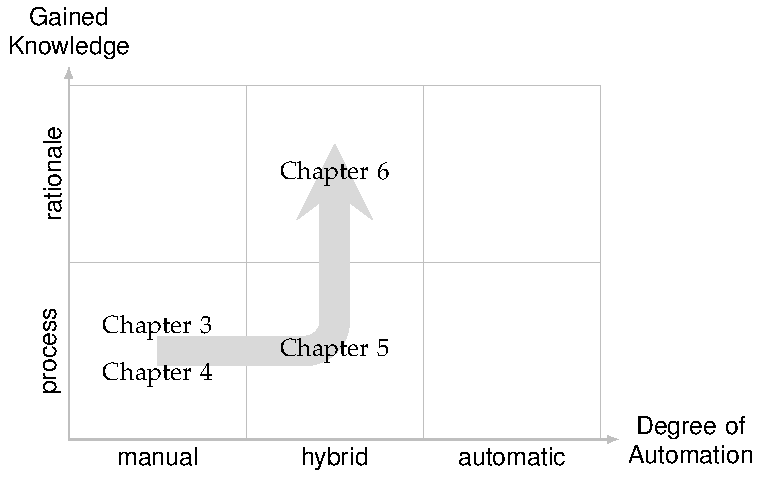
\includegraphics{work}
	\caption{Research problem split by \textcm{data} and \textch{task}. The horizontal axis represents different tasks and the vertical axis represents the complexity involved in the  task. The cells show the characteristics of data will be used to support the task.}
	\label{fig:intro-work}
\end{figure}

The research problem is broken into the following research questions based on the previous data -- task elaboration. They map to the four cells in \autoref{fig:intro-work}. For each question, we explain its context based on the sensemaking-support model described earlier: the sensemaking system, the user, the task and the provenance data. 

\begin{enumerate}
	\item How to design interactive visualizations of \textcm{time-oriented provenance data} 
	enabling users to explore \textch{temporal relationship of sensemaking}?
	
	The domain we target while addressing this research question is \emph{intelligence analysis} -- the original domain that set the foundation for visual analytics research~\cite{Thomas2005}. A common task for intelligence analysts is to examine thousands of reports to identify potential threats from particular persons or organizations. Many visual analytics have been designed to facilitate this analysis. These systems often allow users to take notes, recording the users' thought. We aim to augment these systems by a novel timeline visualization that enables users to identify temporal patterns and construct hidden stories from their annotations.
	
	\item How to design interactive visualizations that can utilize both \textcm{temporal and categorical provenance data} to reveal \textch{complex temporal relationship of sensemaking}?	
	
	This shares the same context with the previous research question. To the best of our knowledge, no existing visualization techniques is designed to show both temporal and categorical information effectively. Therefore, we also aim to design a general timeline visualization that can apply to other domains.
	
	\item How to design interactive visualizations that can exploit \textcm{time-oriented provenance data} to enable users to explore \textch{rational relationship of sensemaking}?
	
	To explore rational relationship of sensemaking, analysts often conduct a user study to observe the process, collect relevant data and analyze it. During the qualitative analysis, analysts may need to go through a lengthy process of transcribing the video recordings before coding the transcript with themes and building model based those themes. In this context, the sensemaking system mapped to \autoref{fig:intro-workflow} can be considered as a set of tools allowing the analysts to conduct a user study and analyze the collected data. We take a different approach to facilitate the transcription and coding steps. We capture analytic provenance while a user performs a sensemaking task and provide visualizations of the provenance data to enable the analyst explore the rational relationship of the user's sensemaking process. We focus only on browser-based sensemaking tasks. The provenance data could include information about visited web pages such as page URL, title and visit time.
	
	\item How to design interactive visualizations that can combine both \textcm{time-oriented provenance data and user-added relations} to enable users to explore \textch{complex rational relationship of sensemaking}?
	
	This research question targets a very common domain: browser-based online sensemaking. To make sense of everyday tasks such as selecting a camera, people often use standard web browsers -- simple sensemaking systems -- to search for different models and consider their strengths and weaknesses. The provenance data could include both automatically captured low-level actions as in the previous question and user-added relationship of the automatic capture such as by spatially grouping them or assigning pair-wise connections.
\end{enumerate}

We take a user-centered design approach in seeking solutions to all the research questions. For each question, we elicit the design requirements by conducting a user study and/or drawing from the literature. Visual encoding and interaction are designed to meet those requirements, and the designs are implemented into a working prototype. Finally, an empirical study is conducted to explore how the tool is used by target audience and check whether it provides the intended support. 

\section{Thesis Contributions}
Toward the overall goal of supporting users in their sensemaking processes through the visualizations of provenance data, this thesis contributes:

\begin{itemize}
	\item A timeline visualization technique -- \emph{\textcb{SchemaLine}} -- that enables users to examine information in chronological order, identify temporal patterns and construct narratives from relevant user annotations. SchemaLine produces a compact but aesthetically pleasing layout and provides a set of fluid interactions allowing users to perform various sensemaking activities described in the Data--Frame model~\cite{Klein2003}. This is to address Research Question 1, and the work is published as 
	
	\textbf{P. H. Nguyen}, K. Xu, R. Walker, and B. L. W. Wong. SchemaLine: Timeline Visualization for Sensemaking. In \textit{International Conference on Information Visualization}, pages 225--233. IEEE, jul 2014.
	
	\item A timeline visualization technique -- \emph{\textcb{TimeSets}} -- that enables users to explore complex temporal relationship by effectively representing both temporal and categorical provenance data. TimeSets visually groups data items that share the same group but still preserves their temporal order. It color codes the backgrounds of the entire groups to distinguish them and uses colored gradient backgrounds for the intersections among those groups. It also adjusts the level of details of each data item dynamically to accommodate more items within a given display estate. This is to address Research Question 2, and the work is published as  
	
	\textbf{P. H. Nguyen}, K. Xu, R. Walker, and B. L. W. Wong. TimeSets: Timeline visualization with set relations. \textit{Information Visualization}, 15(3):253--269, jul 2016. 
	
	and for the VAST Challenge case study as
	
	\item K. Xu, \textbf{P. H. Nguyen}, and B. Fields. Visual analysis of streaming data with SAVI and SenseMAP. In \textit{IEEE Conference on Visual Analytics Science and Technology}, pages 389--390. IEEE, oct 2014.
	 
	\item A visual sensemaking tool -- \emph{\textcb{SensePath}} -- that enables analysts to explore rational relationship of the sensemaking process. Qualitative research methods are often used in understanding rational relationship of sensemaking. This is a manual and time-consuming process: researchers collect observation data, transcribe screen capture videos and think-aloud recordings, identify recurring patterns, and eventually abstract the sensemaking process into a general model. SensePath offers an alternative and possibly faster approach in performing transcription and coding. In stead of having to transcribe the video, SensePath automatically captures and detects participant's sensemaking actions, and provides multi-linked visualizations to support further analysis. It visualizes provenance data in a timeline that enables researchers to quickly gain an overview of the sensemaking process and identify recurring sensemaking patterns. It also links with a screen capture video to allow researchers to examine  additional context when necessary. Finally, to enable researchers to continue working on later stages of analysis using their normal workflow, SensePath exports its coded transcript in a common format that can be used by other popular qualitative data analysis software packages. This is to address Research Question 3, and the work is published as
	
	\textbf{P. H. Nguyen}, K. Xu, A. Wheat, B. L. W. Wong, S. Attfield, and B. Fields. SensePath: Understanding the Sensemaking Process through Analytic Provenance. \textit{IEEE Transactions on Visualization and Computer Graphics}, 22(1):41--50, jan 2016. 
	
	\item A visual sensemaking tool -- \emph{\textcb{SenseMap}} -- that enables users to explore complex rational relationship of sensemaking. It automatically captures and detects sensemaking actions and relationships between these actions before visualizing both of them in a branching history tree. This allows users to examine the rational relationship between the actions they performed and potentially helps them remind of what have been done earlier. SenseMap offers users to assign additional meaning to the automatically collected data by spatially grouping actions or adding rational links between them, in order to help explain complex relationship. Finally, SenseMap allows users to communicate their analysis results at different levels of granularity including a big picture of user-organized findings, a more detailed analysis process and raw provenance data captured. This is to address Research Question 4, and the work is published as 

	\textbf{P. H. Nguyen}, K. Xu, A. Bardill, S. Betul, K. Herd, and B. L. W. Wong. SenseMap: Supporting Browser-based Online Sensemaking through Analytic Provenance. In \textit{IEEE Conference on Visual Analytics Science and Technology}, 2016.
\end{itemize}

Besides the main contributions described in this thesis, I also coauthored two other publications, contributing my knowledge in provenance for sensemaking.

\begin{itemize}
	\item I contributed to the discussion and the design of a framework for provenance in human terrain analysis, and the work was published as
	
	R. Walker, A. Slingsby, J. Dykes, K. Xu, J. Wood, \textbf{P. H. Nguyen}, D. Stephens, B. L. W. Wong, and Y. Zheng. An extensible framework for provenance in human terrain visual analytics. \textit{IEEE Transactions on Visualization and Computer Graphics}, 19(12):2139--2148, dec 2013.
	
	\item I contributed to the organization of a IEEE VIS workshop on provenance for sensemaking. The discussion at the workshop was published as
	
	K. Xu, S. Attfield, T. J. Jankun-Kelly, A. Wheat, \textbf{P. H. Nguyen}, and N. Selvaraj. Analytic provenance for sensemaking: a research agenda. IEEE Computer Graphics and Applications, 35(3):56--64, jan 2015.	
\end{itemize}

\section{Thesis Outline} 
The remainder of this thesis is organized as follows.

First, \autoref{chap:review} reviews the core work related to sensemaking, analytic provenance and visualization. Then, it emphasizes on the visualization of provenance data for supporting sensemaking. At the end, this chapter presents visualization techniques of general time-oriented and network data because these types of data have similar characteristics as provenance data.

\autoref{chap:schemaline} discusses the SchemaLine timeline visualization of user annotations enabling the users to explore temporal relationship of sensemaking -- addressing Research Question 1.

\autoref{chap:timesets} extends \autoref{chap:schemaline} to present the TimeSets visualization technique that can effectively show both temporal and categorical provenance data in order to reveal complex temporal relationship of sensemaking -- addressing Research Question 2.

\autoref{chap:sensepath} discusses the SensePath visualization tool that can exploit time-oriented provenance data, enabling users to explore rational relationship of sensemaking -- addressing Research Question 3.

\autoref{chap:sensemap} describes the SenseMap visualization tool that can utilize both temporal and relational provenance data enabling users to explore complex rational relationship of sensemaking -- addressing Research Question 4.

Finally, \autoref{chap:conclusion} concludes the thesis with a discussion on its contributions and future research directions triggered from this work.
%\chapter{Literature Review}
\label{chap:review}

\graphicspath{{Chapter2/figures/}}

In this chapter, we first discuss the core work in individual topics related to our research problem including sensemaking, visualization and provenance. Then, we focus on their intersection -- analytic provenance -- with capture and visualization of provenance data for supporting sensemaking. Finally, we present visualization techniques of general time-oriented and network data because these two data types are part of our research problem as discussed in \autoref{chap:intro}.

%\section{Sensemaking}
\emph{Sensemaking} reflects how we make sense of the world so that we can act in it~\cite{Snowden2005}. Sensemaking has been studied in many different contexts, most notably including information science~\cite{Dervin1983}, human-computer interaction~\cite{Russell1993}, organizational studies~\cite{Weick1995} and intelligence analysis~\cite{Pirolli2005,Klein2003}. In this section, we review the sensemaking research discussed in these contexts, with an emphasis on the last two sensemaking models that have been highly applied in visualization research. 

\subsection{Gap-Bridging Metaphor}
Dervin develops a sensemaking theory focusing on information seeking and use behaviors~\cite{Dervin1983}. It underlies the cognitive gap that individuals experience when attempting to make sense of observed data. \autoref{fig:lr-dervin} summarizes this \emph{gap-bridging} metaphor. The theory assumes that people moves through time-space in some particular context and situation. Sensemaking starts when they encounter a gap that needs to overcome such as something is unclear or confused. To bridge the gap, they may seek and use information from a variety of sources such as documents, media and other people. These sources are evaluated based on relevant attributes to assess their usefulness. 

\begin{figure}[!htb]
	\centering
	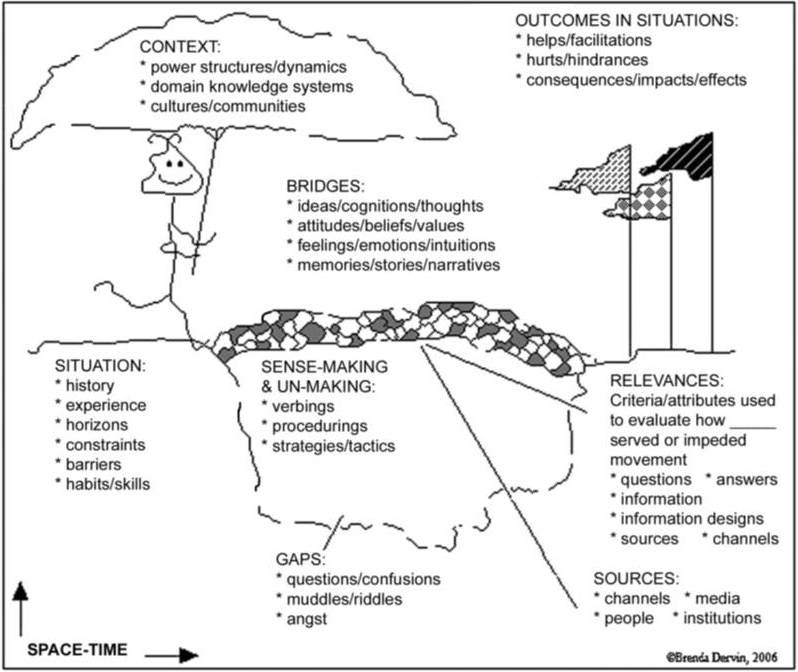
\includegraphics[width=\columnwidth]{dervin}
	\caption{The gap-bridging metaphor of sensemaking. People encounter gaps when moving through time-space, then seek for information, evaluate and use it to bridge the gaps. \is{Dervin2012}}
	\label{fig:lr-dervin}
\end{figure}

Dervin also implements the theory into a set of questions that can be used in interview to understand sensemaking within a context~\cite{Dervin1983}. The questions elaborate all parts of the model, aiming to establish an understanding on the situation (\emph{What happened?}), the gap (\emph{What did you struggle with?}), the bridge (\emph{What idea did you come to?}) and the outcome (\emph{How did that help?}).

\subsection{Learning Loop Complex}
In the context of human-computer interaction, Russell~et~al.~\cite{Russell1993} defines sensemaking as the process of searching for a representation and encoding data in that representation to answer task-specific questions. That cyclic process is called the \emph{learning loop complex} as illustrated in \autoref{fig:lr-russell}. First, the sensemaker searches for a representation to capture salient features of the data (\emph{Generation Loop}). During sensemaking, new information is sought and encoded into this representation (\emph{Data Coverage Loop}). The data unfit to the representation (\emph{residue}) requires the sensemaker to adjusts and produces a more suitable one. This entire learning loop complex is guided by the task with an aim to reduce its cost.

\begin{figure}[!htb]
	\centering
	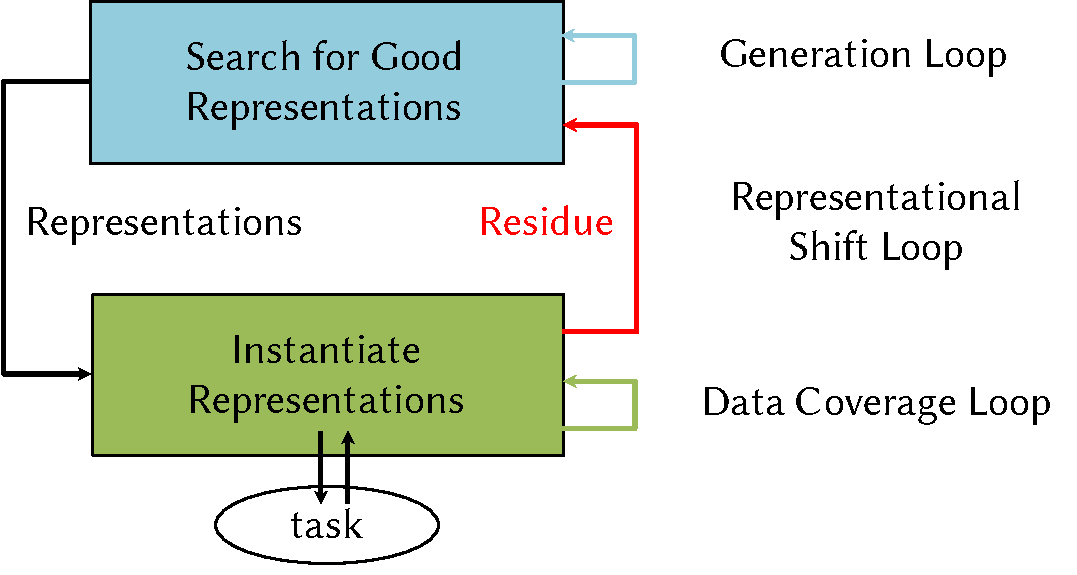
\includegraphics{russell}
	\caption{The learning loop complex theory of sensemaking. It consists of three iterative loops: searching for a good representation, encoding data to the representation, and adjusting the representation for a better data coverage. \is{Russell1993}}
	\label{fig:lr-russell}
\end{figure}

\subsection{Sensemaking in Organizations}
Different from Dervin and Russell who study sensemaking for individuals, Weick focuses on sensemaking at an organization level~\cite{Weick1995}. He proposes that sensemaking consists of these seven following properties.

\begin{enumerate}
	\item \emph{Grounded in identity construction}. Who people think they are, both individually and collectively, affect what they interpret and act.
	\item \emph{Retrospective}. People look back and make sense from what they have said and what they have done before.
	\item \emph{Enactive of sensible environments}. People make sense and contribute to the environments during their sensemaking processes.
	\item \emph{Social}. This is an inherent property of sensemaking in organization where people interact and socialize with others, and also are influenced by others.
	\item \emph{Ongoing}. Sensemaking is a continuous flow because the world and our understanding about the word are constantly changing.
	\item \emph{Focused on and by extracted cues}. Cues are things from the context that people have attention to and may use them to guide further exploration and assessment of the sensemaking problem.
	\item \emph{Driven by plausibility rather than accuracy}. Sensemaking is about plausibility and sufficiency rather than accuracy and completeness. People tend to stop searching when they find an acceptable solution.
\end{enumerate}

\subsection{A Process Model}
\label{sub:lr-pcm}
Pirolli and Card~\cite{Pirolli2005} describe sensemaking as an iterative process that gradually transforms raw data into rational knowledge. The process includes two sets of activities: one that cycles around finding relevant information, and another that cycles around making sense of that information, with plenty of interaction between them. They map to the \emph{foraging loop} and the \emph{sensemaking loop} respectively, as shown in \autoref{fig:lr-pirolli-card-model}. The sensemaking process can progress upward (from data to knowledge) or downward (from knowledge to data). The steps in the \emph{bottom-up} process are summarized as follows.

\begin{figure}[!htb]
	\centering
	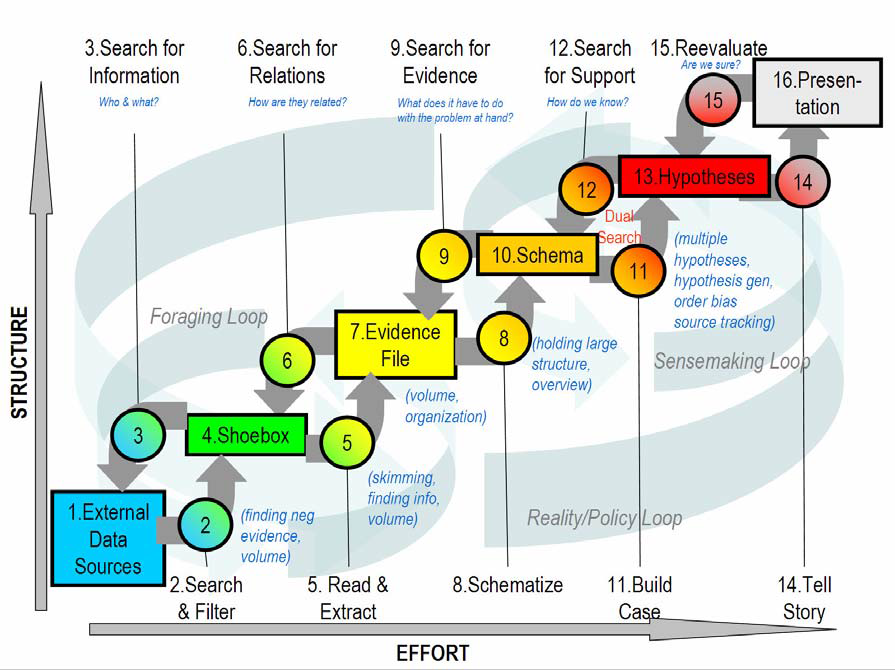
\includegraphics[width=\columnwidth]{pirolli-card-model}
	\caption{A notional model of sensemaking. The sub-processes (numbered circles) and their data input/output (numbered rectangles) are arranged in a two-dimensional space, in which the horizontal axis represents the degree of effort from users, and the vertical axis represents the degree of structure in information representation. \is{Pirolli2005}}
	\label{fig:lr-pirolli-card-model}
\end{figure}

\begin{itemize}
	\item \emph{Search and filter}. External data sources, such as classified databases or the web, are searched and filtered to retrieve relevant documents to the task.
	\item \emph{Read and extract}. These documents are examined to extract pieces of information that may be used as evidence later.
	\item \emph{Schematize}.  The collected information is organized in a way that aids the analysis. This may be executed in user mind, using paper and pen, or with a complex computer-based system.
	\item \emph{Build case}. Multiple hypotheses are generated; evidence are marshaled to support or disconfirm them.
	\item \emph{Tell story}. Discovered cases are presented to some audience.
\end{itemize}

In this model, \emph{schematization} plays an important role in converting raw evidence to rational explanations, bridging the foraging and sensemaking loops. A study by Kang, Görg and John Stasko~\cite{Kang2011} agrees with this observation. In their study, all the participants who performed the sensemaking task well spent considerable time and effort in organizing their collected information. Their organizational schemes were flexible: a \emph{timeline} of related events, a \emph{map} connecting locations that a person has been to, and a \emph{diagram} showing relationships among suspicious targets.

\subsection{Data--Frame Model}
\label{sub:lr-dfm}
Klein et al.~\cite{Klein2003} propose a sensemaking model that centers around \emph{data} and \emph{frame}. Data is the information that a person receives or searches for, and frame is the mental structure that organizes and explains the relationship of such data. For instance, a frame can be a \emph{story}, explaining the chronology of events and the causal relationships between
them; or a \emph{map}, showing where the events take place and the routes between them. Sensemaking is considered as a deliberate effort to understand an event, starting when a person realizes a gap of their current understanding of that event. Klein and his associates describe seven activities involved in sensemaking and are summarized in \autoref{fig:lr-data-frame-model}.

\begin{figure}[!htb]
	\centering
	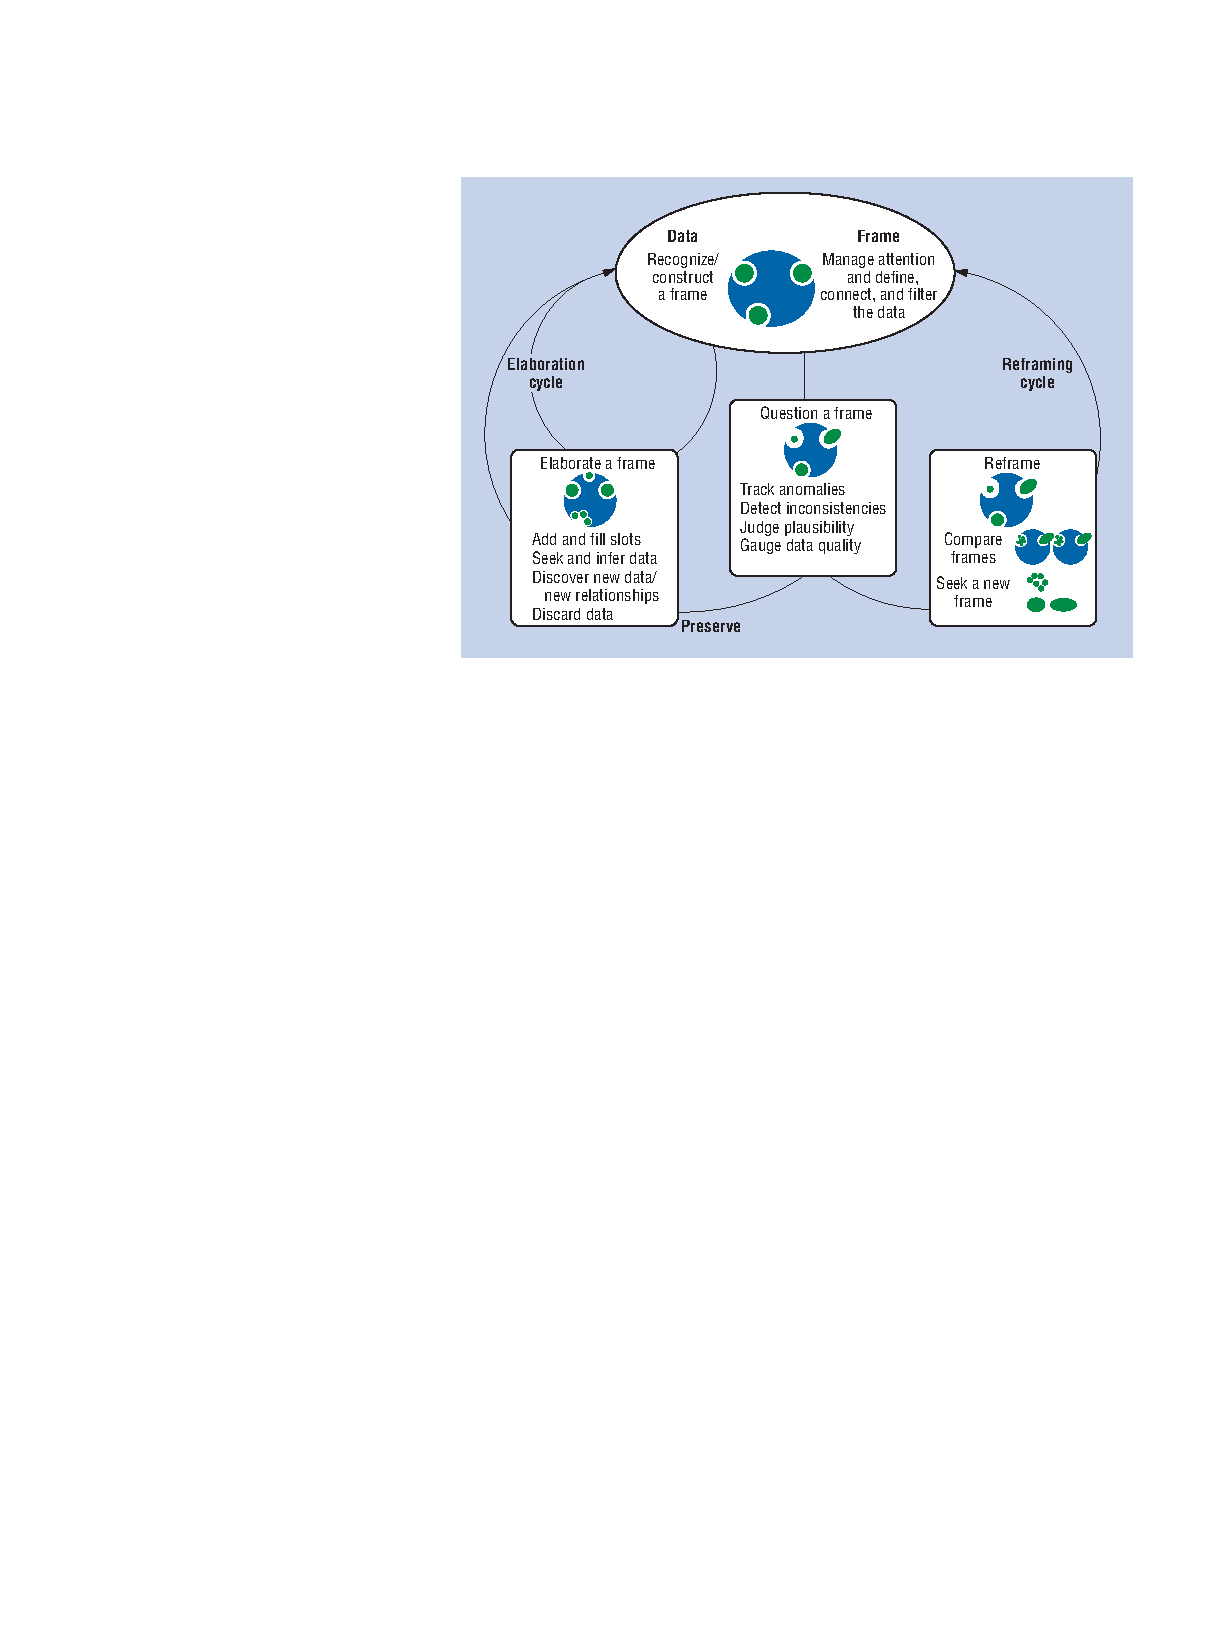
\includegraphics[width=\columnwidth]{data-frame-model}
	\caption{The data--frame model of sensemaking. It describes a set of interconnected sensemaking activities centering around data and frame -- the explanatory structure of data. \is{Klein2003}}
	\label{fig:lr-data-frame-model}
\end{figure}

\begin{itemize}
	\item \emph{Connect data and a frame}. A person recognizes relevant pieces of data and constructs an initial frame to explain them. The frame then helps the person to filter and search for new data.
	\item \emph{Elaborate the frame}. As more is learned about the situation, the frame becomes more elaborate with new data and new relationships. 
	\item \emph{Question the frame}. It happens when a person encounters data that is inconsistent with the existing frame. At this point, the person may be unsure that the frame is incorrect, or the inconsistent data is inaccurate.
	\item \emph{Preserve the frame}. A person may consider the severity of the inconsistent data, justify why it mismatches the frame, and ignore it.
	\item \emph{Compare multiple frames}. Depending on experience, a person may think of alternative frames explaining the same set of data. These frames need to be compared to select the most likely one.
	\item \emph{Reframe}. When encountering inconsistent and contrary data, the person may need to find a replacement that can explain all data. Considering discarded data and/or reinterpreting data could facilitate this activity.
	\item \emph{Seek a new frame}. A person may deliberately search for a new frame when encountering plenty of conflicted data. One or two key data elements may serve as \emph{anchors} to help the person to elicit another frame.
\end{itemize}

The Pirolli and Card's model describes a step-by-step process of sensemaking, in which the analyst collects relevant data and eventually transposes it into rational answers. However, the various sensemaking activities in the Data--Frame model may explain the strategies used by the analyst more comprehensively.

TODO: summary
A recent and comprehensive review of sensemaking can be found in the article by Maitlis and Christianson~\cite{Maitlis2014}. 
\section{Visualization and Visual Analytics}

\subsection{Overview}
Computer-based visualization systems provide visual representations of datasets designed to help people carry out tasks more effectively~\cite{Munzner2014}. Because the design space of possible visual ``idioms'' is huge, it is challenging to create effective visualizations. Understanding well-established information design principles and interaction techniques could guide designers toward the right direction. Also, every visualization needs to be evaluated to check whether it meets its design purposes and how it helps or hinder users.

Overview: what is vis? what can vis help? what is VA? what can VA help, in addition to vis? explain the VA process model. briefly explain the 3 important blocks in the model, which are then discussed in detail next. 

%What is vis? Classic example. What vis can help from cognition (Ben) and Wijk, Fekete?
%
%Large datasets -> simple aggregation, reduction like filtering, interaction, ; larger datasets, more sophiscated emthods extract patterns and vis to display them. and allow further. That is the idea of visual analytics. Orginal def, new def. Model.
%
%Describe visual analytics process model (Figure~\ref{fig:visual-analytics-process})
%
%\begin{figure}[!htb]
%	\centering
%	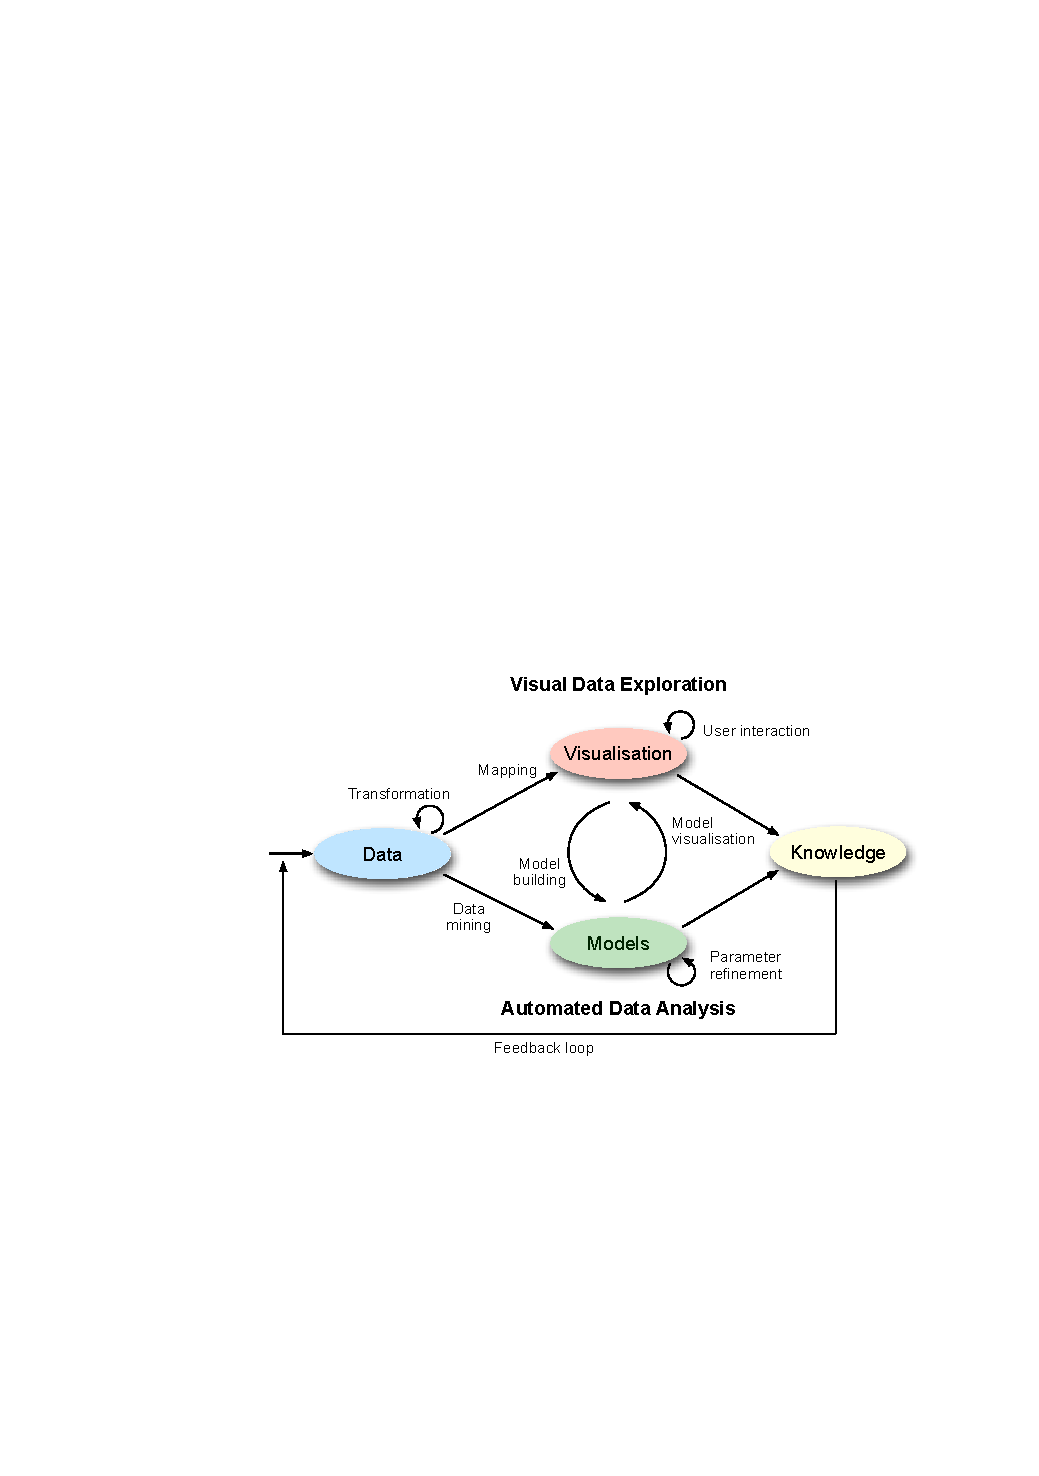
\includegraphics[width=\columnwidth]{visual-analytics-process}
%	\caption{The visual analytics process model. \emph{Source:~\cite{Keim2010}}.}
%	\label{fig:visual-analytics-process}
%\end{figure}
%
%
%Next, discuss basics of vis and models. and evaluation.

\subsection{Visualization Design}


\subsubsection{Information Design Principles}
\label{sub:lr-design}

\paragraph{Marks and Channels}
Marks are basic geometric elements that depict items or links, and channels control their appearance~\cite{Munzner2014}. Item marks can be zero-dimensional as a \emph{point}, one-dimensional as a \emph{line}, two-dimensional as an \emph{area}, and three-dimensional as a \emph{volume}, but rarely used. Link marks include \emph{connection} showing a pairwise relationship between two items using a line and \emph{containment} showing hierarchical relationships using areas. \autoref{fig:lr-marks} illustrates these marks. 

\begin{figure}[!htb]
	\centering
	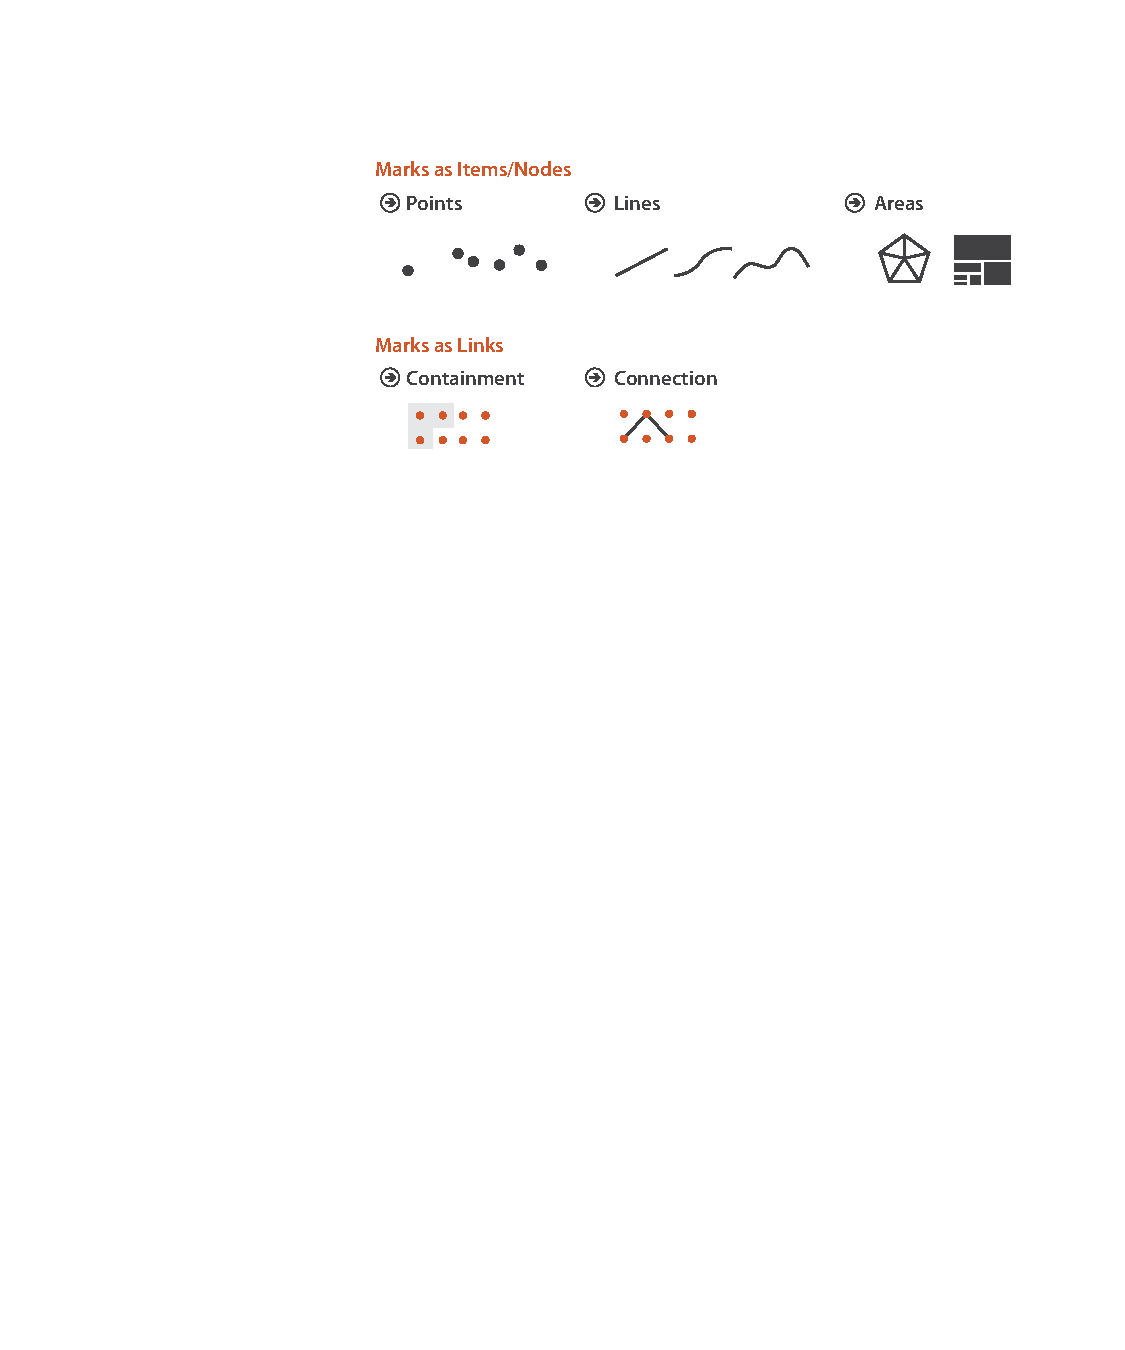
\includegraphics[width=.8\linewidth]{marks}
	\caption{Item and link marks as geometric primitives. \is{Munzner2014}}
	\label{fig:lr-marks}
\end{figure}

A visual channel control the appearance of marks, independent of their dimensionality. Examples include position, color, shape, angle and size. However, not all channels can be applied to all marks. For instance, an area mark is used in a geographic map to denote a region. It is already associated with a shape and size, thus cannot be size coded to represent another quantitative attribute.
some visual channels. some cannot encode size, example. \autoref{fig:lr-channel-example} shows a progression of chart types, with each showing one more data attribute using one more visual channel. \autoref{fig:lr-channel-example-1} shows a bar chart representing a single quantitative attribute using the \emph{vertical position} channel. \autoref{fig:lr-channel-example-2} shows a scatter plot encoding the second quantitative attribute using the \emph{horizontal position} channel. \autoref{fig:lr-channel-example-3} adds the \emph{color} channel to represent a categorical attribute, and \autoref{fig:lr-channel-example-4} adds the \emph{size} channel to represent another quantitative attribute. In these examples, each attribute is encoded with a single channel. However, multiple channels can be combined to redundantly encode the same attribute, helping perceive it more easily.

\begin{figure}[!htb]
\centering
\subcaptionbox{Line marks with horizontal position for a categorical attribute and vertical position for a quantitative attribute.\label{fig:lr-channel-example-1}}{
\includegraphics[width=.23\columnwidth]{channel-example-1}} 
\hfill
\subcaptionbox{Point marks with both horizontal and vertical position channels for quantitative attributes.\label{fig:lr-channel-example-2}}{
\includegraphics[width=.23\columnwidth]{channel-example-2}} 
\hfill
\subcaptionbox{A categorical attribute is added using the color channel.\label{fig:lr-channel-example-3}}{
\includegraphics[width=.23\columnwidth]{channel-example-3}}
\hfill
\subcaptionbox{Another quantitative attribute is added using the size channel.\label{fig:lr-channel-example-4}}{
\includegraphics[width=.23\columnwidth]{channel-example-4}}
\caption{Using marks and channels.}
\label{fig:lr-channel-example}
\end{figure}

All channels are not equal; they are processed and perceived differently by our human visual systems. Also, not all channels are appropriate for encoding both ordered and categorical attributes. Ordered attributes should be shown using magnitude channels, with \emph{aligned spatial position} as the most effective channel and \emph{3D volume} as the least effective one. Categorical attributes should be shown using identity channels, with \emph{spatial region} as the most effective channel and \emph{shape} as the least effective one. \autoref{fig:lr-channel-ranking} shows the detailed ranking of effectiveness of many visual channels, separated by the type of attribute. This ranking is documented by Munzner~\cite{Munzner2014}, based on many empirical studies such as the work by Cleveland and McGill~\cite{Cleveland1985}, and by Heer and Bostock~\cite{Heer2010a}.

\begin{figure}[!htb]
	\centering
	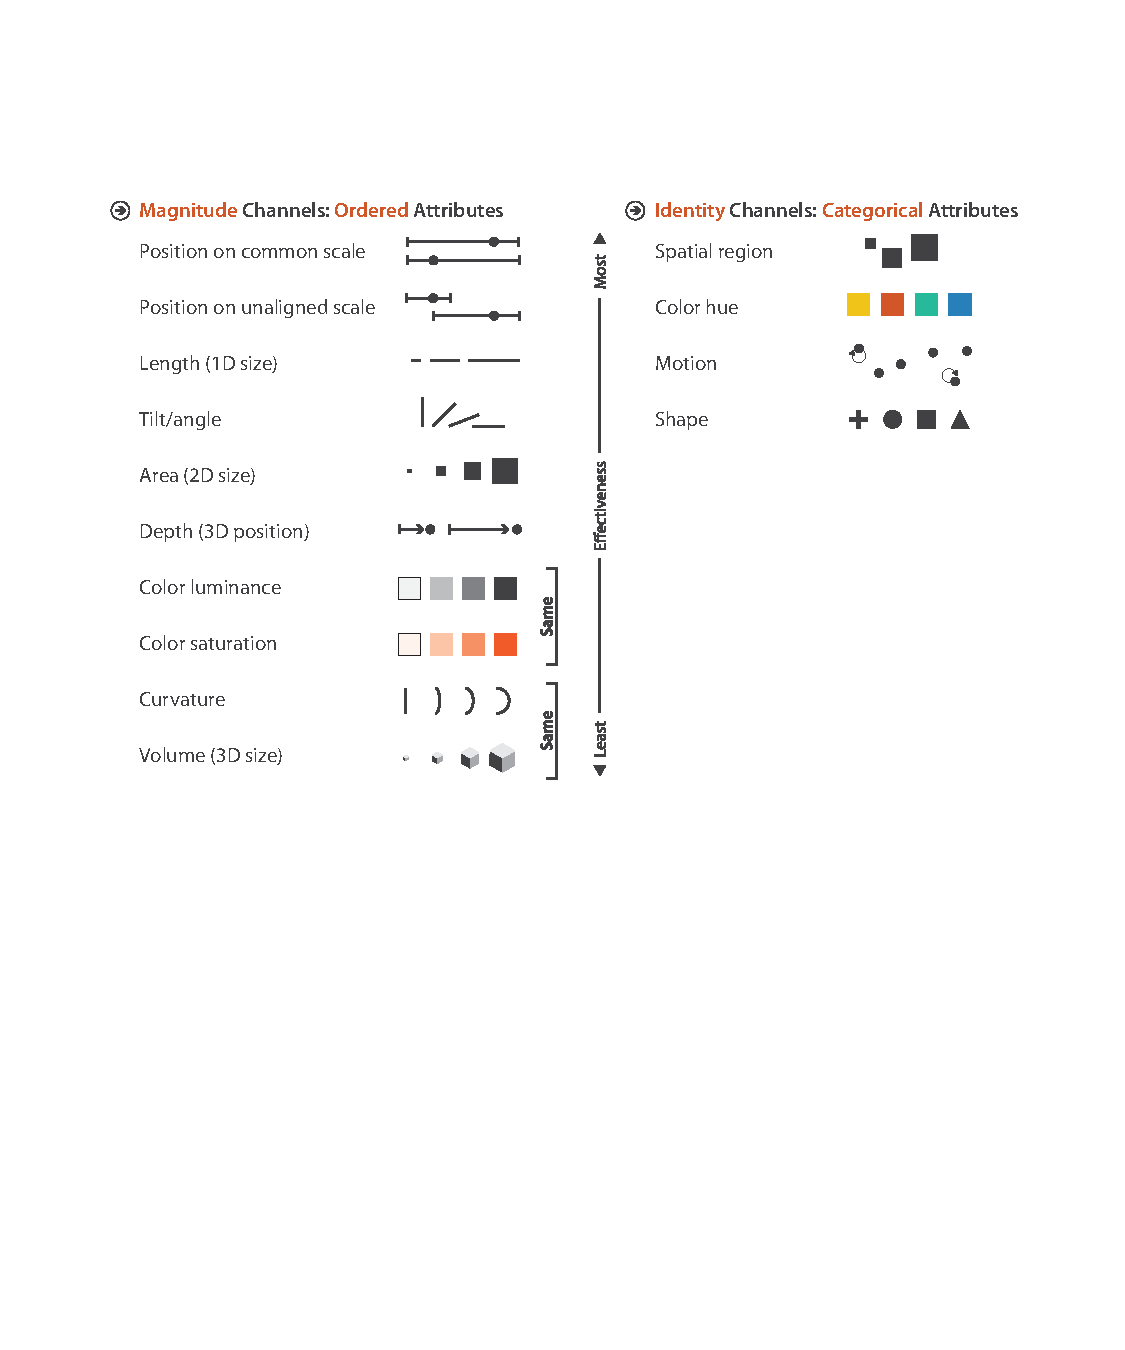
\includegraphics[width=\linewidth]{channel-ranking}
	\caption{Channels ranked by effectiveness according to data and channel type. \is{Munzner2014}}
	\label{fig:lr-channel-ranking}
\end{figure}

Color is a special channel that can be used for both data attributes. As shown in \autoref{fig:lr-channel-ranking}, color luminance and saturation are used in magnitude channels, and color hue is used in identity channels. A colormap specifies a mapping between colors and data values, and designing an effective colormap is challenging. ColorBrewer~\cite{Harrower2003} is an excellent source for colormap reference, providing color schemes for both categorical and ordered attributes. Human can only distinguish around 12 colors simultaneously~\cite{Munzner2014}. \autoref{fig:lr-colorbrewer-1} shows such a categorical colormap with 12 distinguished color hues. Ordered colormaps can be either sequential (\autoref{fig:lr-colorbrewer-2}) or diverging (\autoref{fig:lr-colorbrewer-3}). Diverging colormaps use two different color hues to emphasize values below and above the middle point.

\begin{figure}[!htb]
\centering
\subcaptionbox{Categorical colormap with distinguishable color hues.\label{fig:lr-colorbrewer-1}}[\columnwidth]{
\includegraphics[width=.6\columnwidth]{colorbrewer-1}} 
\\
\subcaptionbox{Sequential colormap: a single color hue with different saturation level.\label{fig:lr-colorbrewer-2}}[\columnwidth]{\hspace{-.15\columnwidth}
\includegraphics[width=.45\columnwidth]{colorbrewer-2}}
\\
\subcaptionbox{Diverging colormap: two color hues emphasizing positive and negative values.\label{fig:lr-colorbrewer-3}}[\columnwidth]{\hspace{-.05\columnwidth} 
\includegraphics[width=.55\columnwidth]{colorbrewer-3}}
\caption{Colormaps from ColorBrewer. \is{Harrower2003}}
\end{figure}

\subparagraph{Gestalt Principles}
\label{sub:lr-gestalt}
Gestalt principles describe how we see patterns in visual displays~\cite{Koffka1935}. This section reviews three commonly used principles in representing groups of items.

\subparagraph{Similarity} 
Similar elements tend to be grouped together. \autoref{fig:lr-gestalt-similarity-1} shows a matrix of point marks with uniform spacing, but using two different shapes: dot and cross. The similarity of shapes helps us see the rows more clearly than the columns. Two separable channels can be applied together to reveal patterns by either rows or columns. In \autoref{fig:lr-gestalt-similarity-2}, green is used to depict rows, and texture is used to depict columns.

\begin{figure}[!htb]
\centering
\subcaptionbox{Similarity of shapes distinguishes rows.\label{fig:lr-gestalt-similarity-1}}[.47\columnwidth]{
\includegraphics[height=.35\columnwidth]{gestalt-similarity-1}} 
\hfill
\subcaptionbox{Color and texture delineate rows and columns, respectively.\label{fig:lr-gestalt-similarity-2}}[.47\columnwidth]{
\includegraphics[height=.35\columnwidth]{gestalt-similarity-2}} \label{fig:lr-gestalt-similarity}
\caption{Similarity principle: similar elements are perceived as a group. \is{Ware2013}}
\end{figure}

\subparagraph{Proximity} 
Elements that are close together are perceptually grouped together. \autoref{fig:lr-gestalt-proximity-1} clearly shows two groups of dots. \autoref{fig:lr-gestalt-proximity-2} shows rows of dots. However, with a small change of spacing, these dots are perceived as columns in \autoref{fig:lr-gestalt-proximity-3}. The application of this principle is straightforward: organizing related information close together. It helps separate groups of unrelated objects and facilitates searching for information.

\begin{figure}[!htb]
\centering
\subcaptionbox{Two groups of dots.\label{fig:lr-gestalt-proximity-1}}{
\includegraphics[width=.25\columnwidth]{gestalt-proximity-1}} 
\hfill
\subcaptionbox{Rows of dots.\label{fig:lr-gestalt-proximity-2}}{
\includegraphics[width=.31\columnwidth]{gestalt-proximity-2}} 
\hfill
\subcaptionbox{Columns of dots.\label{fig:lr-gestalt-proximity-3}}{
\includegraphics[width=.31\columnwidth]{gestalt-proximity-3}}
\label{fig:lr-gestalt-proximity}
\caption{Spatial proximity principle: spatially close elements are perceived as a group. \is{Ware2013}}
\end{figure}

\paragraph{Connectedness} 
Elements that are connected by visual properties are perceived as being more related than elements that are not connected. This principle can be achieved simply by drawing a border around a group of elements as in \autoref{fig:lr-gestalt-connectedness-1}. This is extensively applied in designing complex graphical user interface: groups of related features are separated by borders. Another approach to implement connectedness is by drawing lines between related elements as in \autoref{fig:lr-gestalt-connectedness-2}. This is the basics of \emph{node-link diagrams} -- one of the most common methods of representing relationships between elements.

\begin{figure}[!htb]
\centering
\subcaptionbox{Using border to denote a group.\label{fig:lr-gestalt-connectedness-1}}{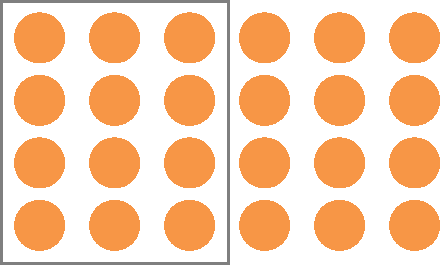
\includegraphics[width=.4\columnwidth]{gestalt-connectedness-1}} 
\hfill
\subcaptionbox{Using lines to denote a group.\label{fig:lr-gestalt-connectedness-2}}{
\includegraphics[width=.4\columnwidth]{gestalt-connectedness-2}} 
\caption{Connectedness principle: visually connected elements are perceived as a group. \is{Ware2013}}
\label{fig:lr-gestalt-connectedness}
\end{figure}

Among these three Gestalt principles of representing groups of elements, connectedness has the strongest effect, followed by proximity and then similarity. \autoref{fig:lr-gestalt} illustrates this comparison. In \autoref{fig:lr-gestalt-1}, even though spacing between dots in rows is shorter than spacing between dots in columns, the lines make the vertical links clearer than rows. In \autoref{fig:lr-gestalt-2}, the lines also make the horizontal links more notable than groups of colored circles. In \autoref{fig:lr-gestalt-3}, two spatial groups are more clearly perceived than colored groups.

\begin{figure}[!htb]
\centering
\subcaptionbox{Links are more clearly perceived than spatial groups.\label{fig:lr-gestalt-1}}[.3\columnwidth]{
\includegraphics[height=.12\columnwidth]{gestalt-1}} 
\hfill
\subcaptionbox{Links are more clearly perceived than colored groups.\label{fig:lr-gestalt-2}}[.3\columnwidth]{
\includegraphics[height=.12\columnwidth]{gestalt-2}} 
\hfill
\subcaptionbox{Spatial groups are more clearly perceived than colored groups.\label{fig:lr-gestalt-3}}[.3\columnwidth]{
\includegraphics[height=.12\columnwidth]{gestalt-3}}
\caption{Comparison of Gestalt principles. Connectedness is stronger than proximity, and proximity is stronger than similarity. \is{Ware2013}}
\label{fig:lr-gestalt}
\end{figure}

\paragraph{Tufte's Principles}
Tufte proposes a number of principles for a well-designed graphic, documented in his series of books, most notably including \emph{The Visual Display of Quantitative Information}~\cite{Tufte1983} and \emph{Envisioning Information}~\cite{Tufte1990}. This section reviews a few principles that have been commonly applied in graphic design and visualization.

\subparagraph{Graphical Integrity}
This principle emphasizes that the graphical representation should tell the truth about the data. Representation of numbers, as physically measured on the surface of the	graphic	itself,	must be directly proportional to the numerical quantities represented~\cite{Tufte1983}. \autoref{fig:lr-tufte-integrity-1} shows a falsely big drop in stock market value between 2001 and 2002. It because the chart uses a relative scale with the value range from 450 to 500, causing its height disproportional to the market value. \autoref{fig:lr-tufte-integrity-2} corrects this error by using an absolute scale with the value range starting from 0.

\begin{figure}[!htb]
\centering
\subcaptionbox{Using a relative value range causes a falsely big drop of stock market value between 2001 and 2002.\label{fig:lr-tufte-integrity-1}}{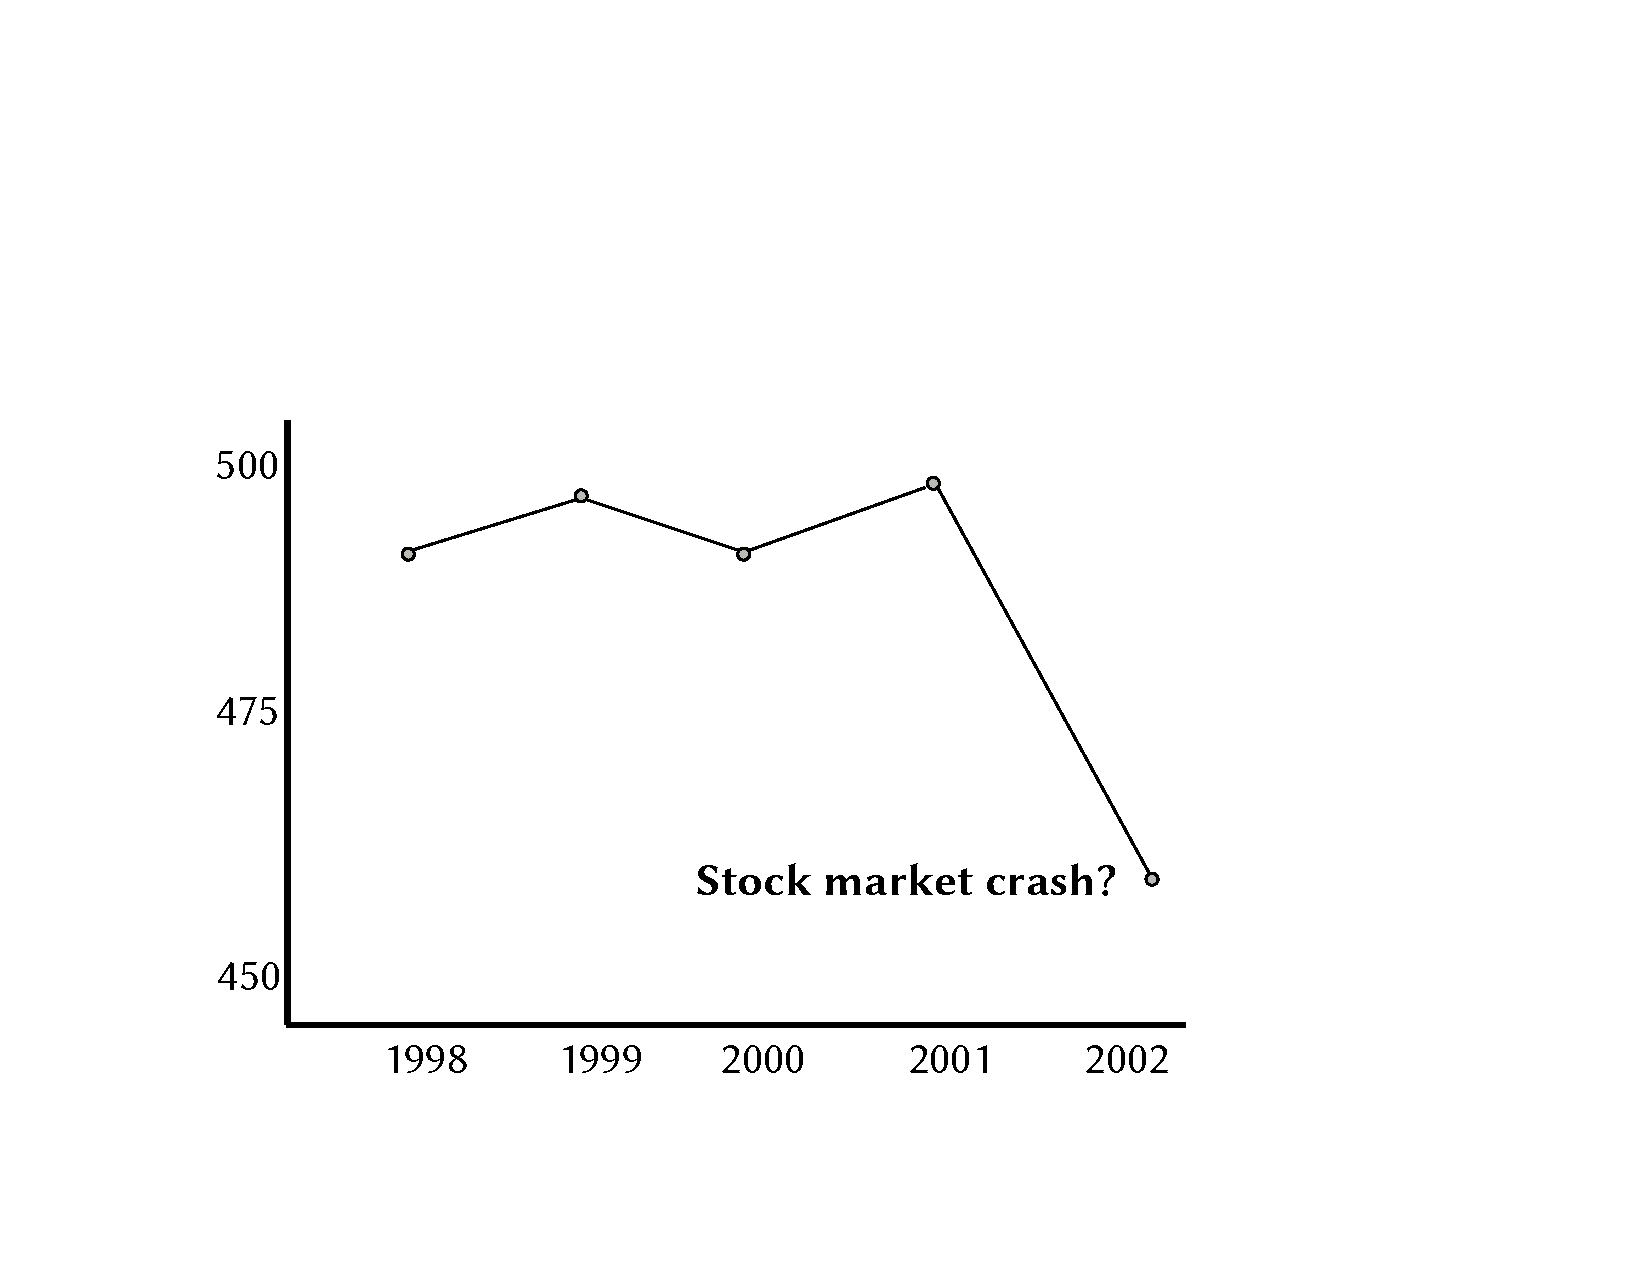
\includegraphics[width=.47\columnwidth]{tufte-integrity-1}} 
\hfill
\subcaptionbox{Using an absolute value range to depict the data accurately.\label{fig:lr-tufte-integrity-2}}{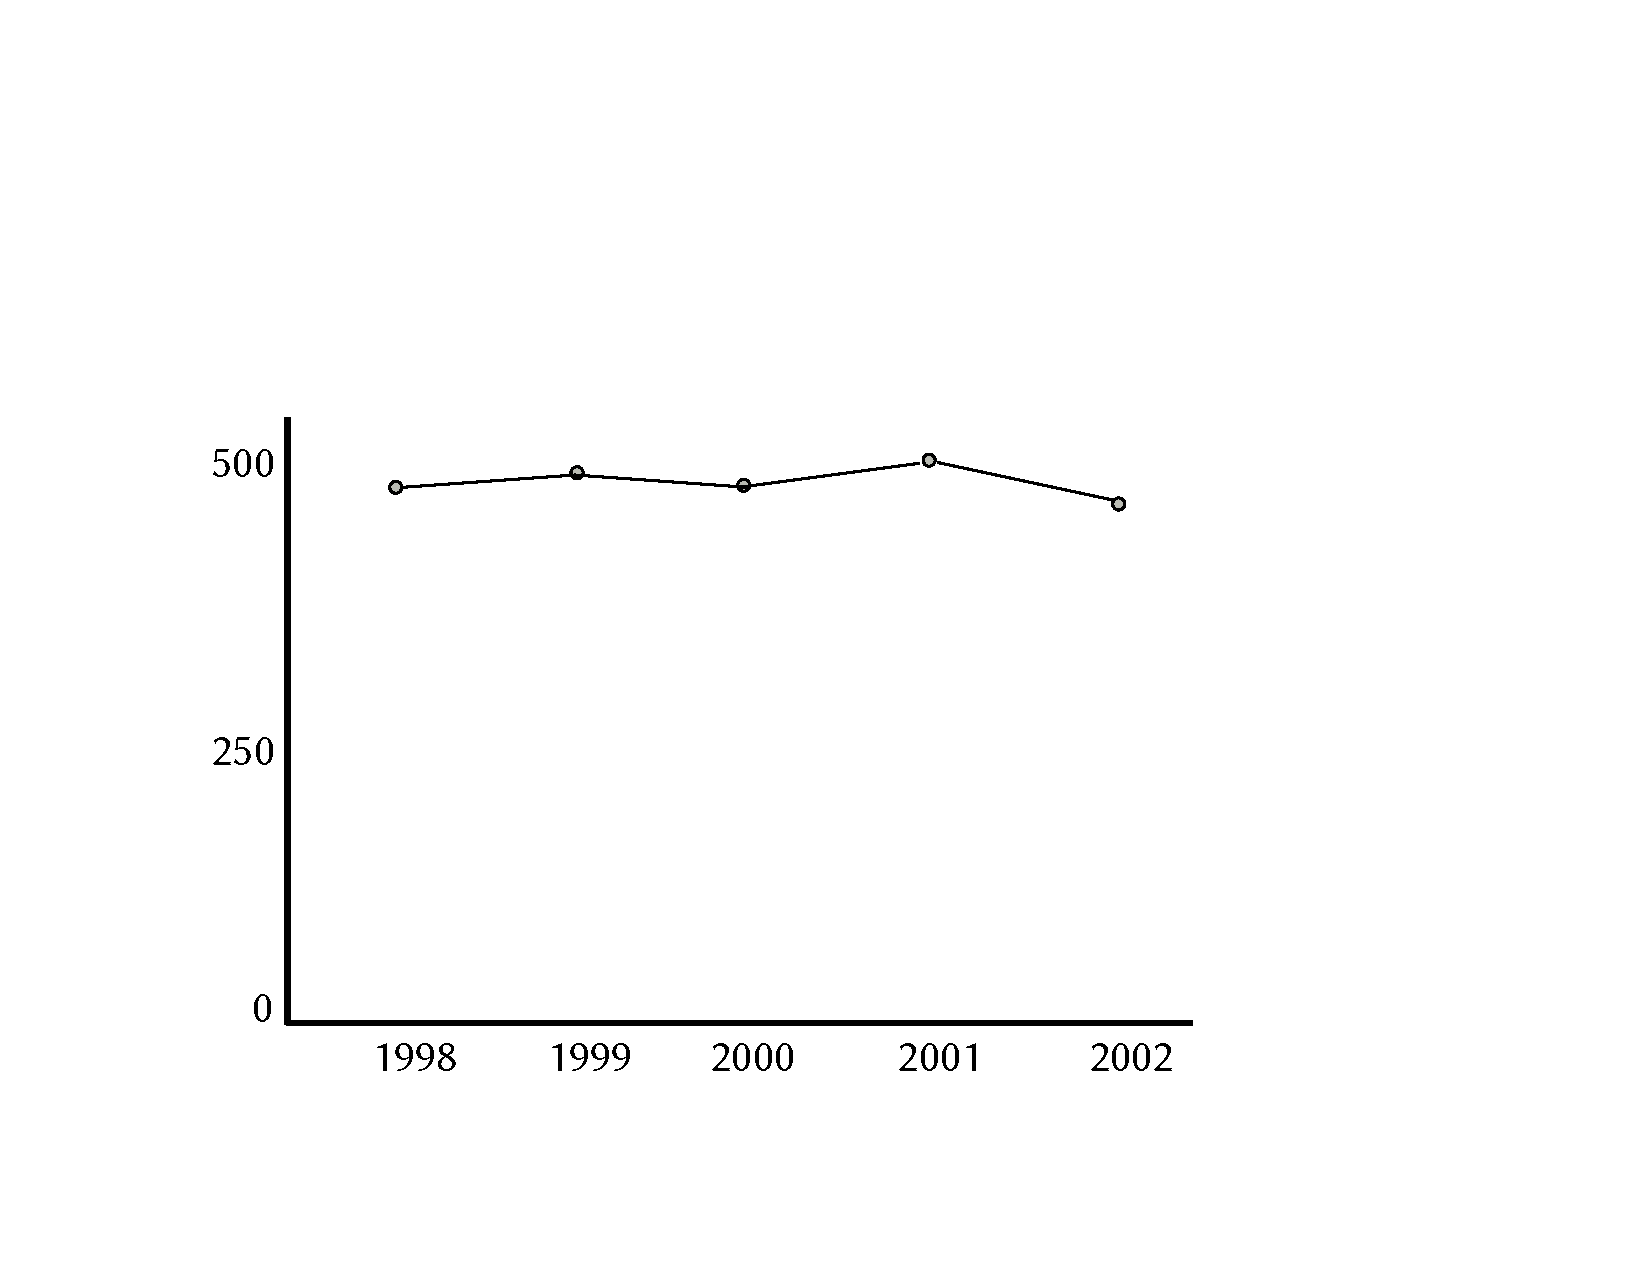
\includegraphics[width=.47\columnwidth]{tufte-integrity-2}} 
\caption{Graphical integrity principle. The chart should tell the truth about the data.}
\label{fig:lr-tufte-integrity}
\end{figure}

\subparagraph{Data-Ink Ratio Maximization}
Data-ink includes the pixels in the graphic that are used for representing the data. Data-ink ratio is defined as the ratio between the data-ink and the total non-background pixels used in the graphic. This principle aims to maximize this ratio by erasing non-data-ink and erasing redundant data-ink.

\begin{figure}[!htb]
\centering
\subcaptionbox{A bar chart with poor data-ink ratio.\label{fig:lr-tufte-ink-1}}{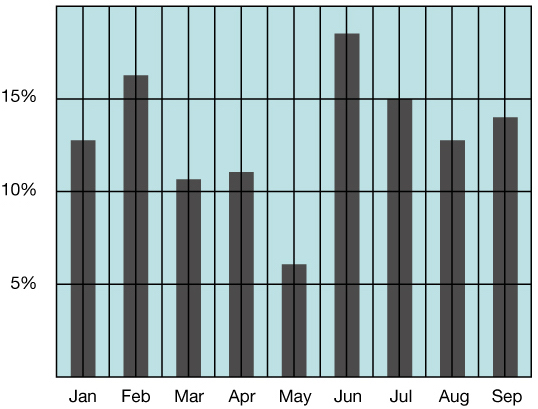
\includegraphics[width=.47\columnwidth]{tufte-ink-1}} 
\hfill
\subcaptionbox{A bar chart with high data-ink ratio by removing background, border and grid lines.\label{fig:lr-tufte-ink-2}}{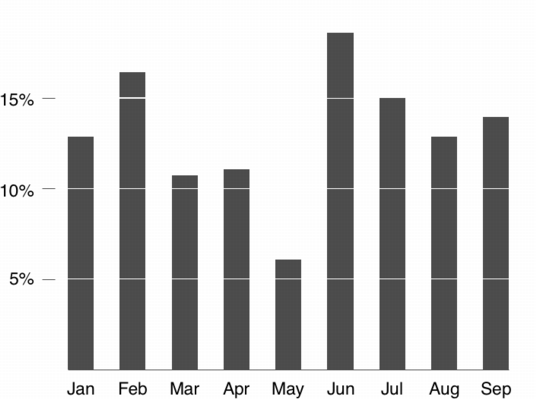
\includegraphics[width=.47\columnwidth]{tufte-ink-2}} 
\caption{Data-ink ratio maximization principle: removing the graphic that does not contribute to the understanding of the data.}
\label{fig:lr-tufte-ink}
\end{figure}
% Source: http://www.infovis-wiki.net/index.php/Data-Ink_Ratio

\subparagraph{Micro/Macro Readings}
This principle suggests that a graphic can contain both enormous details and an overall pattern. This allows the viewer to glance from a distance to observe the big picture, and later drill-down closely to examine its individual pieces. Classic stem-and-leaf plot is a great example to illustrate this principle (\autoref{fig:lr-tufte-micro}). The plot shows all individual data items at meaningful level of detail, and provides an understanding of the data distribution. The micro/macro principle is extensively applied in interactive visualization, where zooming are panning are made possible, such as Google Maps. Data items at different scales can be represented with different levels of detail to provide appropriate information based on the allowed display area.

\begin{figure}[!htb]
	\centering
	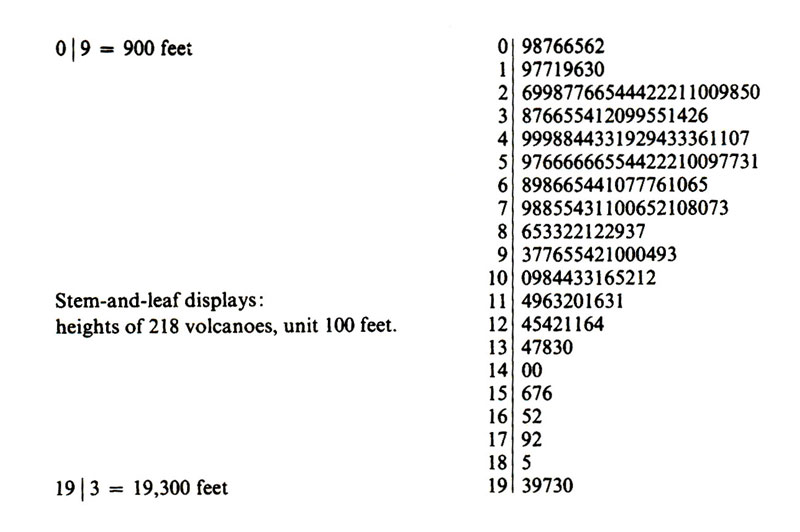
\includegraphics[width=.9\linewidth]{tufte-micro}
	\caption{Micro/macro principle. A stem-and-leaf plot shows both the data distribution and individual items. \is{Tufte1983}}
	\label{fig:lr-tufte-micro}
\end{figure}


%In a broader context, GUI design principles:  Schneiderman~\cite{Shneiderman2016} (eight golden rules), Norman (six design principles) ~\cite{Norman2002} and	Nielsen (ten usability heuristics)~\cite{Nielsen1994} -- create a table with rows showing similar principles
%http://www.csun.edu/science/courses/671/bibliography/preece.html
%https://faculty.washington.edu/jtenenbg/courses/360/f04/sessions/schneidermanGoldenRules.html
%https://www.interaction-design.org/literature/article/shneiderman-s-eight-golden-rules-will-help-you-design-better-interfaces

\subsubsection{Interaction Techniques}
Interaction typically refers to the set of controls provided to the user to manipulate an interface~\cite{Pike2009a}. A static visualization may only show one aspect of a dataset. When the dataset is large enough, showing all the data at once may also make the visualization become cluttered. Interaction plays an important role in solving these problems. It can help explore large datasets at multiple levels of detail, identify patterns through examination of different visual representations and understand the connections between them.

Examples of interaction include standard techniques used in graphical user interface such as mouse clicking and scrolling, and more visualization specific techniques such as \emph{linking and brushing}~\cite{Kosara2003}, and \emph{focus+context}~\cite{Cockburn2008}. Multiple views in a visualization are often linked together to exploit their strengths. The user can select points of interest using the brushing technique, typically done directly on the visual data representation such as dragging a rectangular area. The points are brushed in one view will be highlighted in other views, allowing the user to explore them with different perspectives and representations (\autoref{fig:lr-linking}). Focus+Context is a technique that brings both the overview (context) and the detailed information (focus) together in one view. A fisheye view~\cite{Furnas1986,Furnas2006} is one example of this technique: the focal region is magnified and displayed within its surrounding context (\autoref{fig:lr-fisheye}).

\begin{figure}[!htb]
\centering
\subcaptionbox{Linking and brushing. Data points brushed in one view are linked and highlighted in other views.\label{fig:lr-linking}}{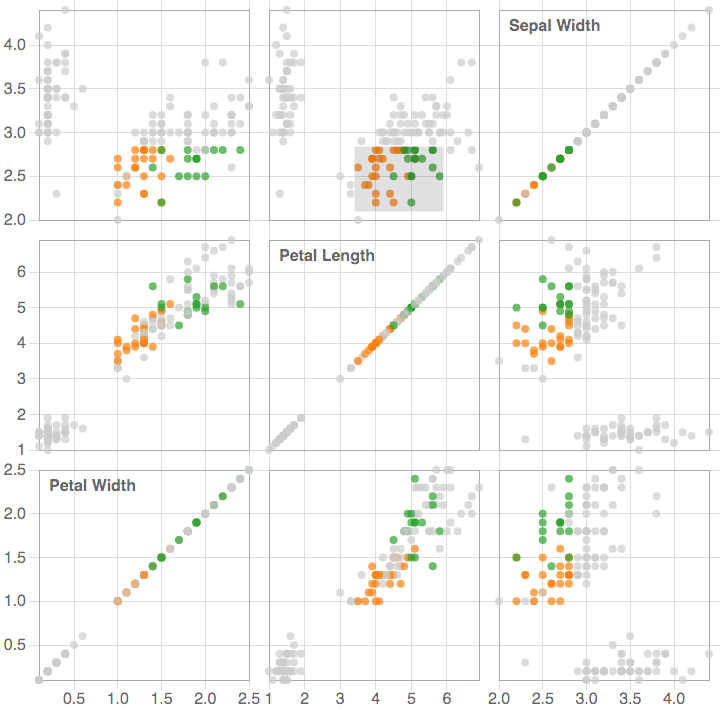
\includegraphics[height=.43\columnwidth]{linking}} 
\hfill
\subcaptionbox{Fisheye view for focus+context. Both the overview and the detailed information are displayed in one view.\label{fig:lr-fisheye}}{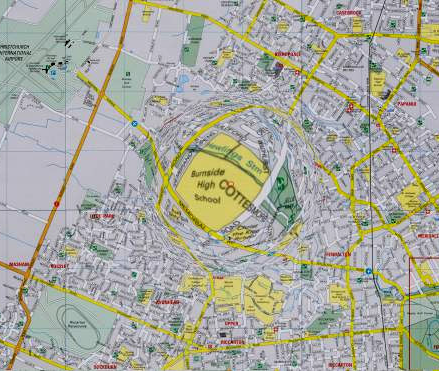
\includegraphics[height=.43\columnwidth]{fisheye}} 
\caption{Examples of interaction techniques.}
\label{fig:lr-interaction}
\end{figure}

Many other interaction techniques can be found in the taxonomies by Dix and Ellis~\cite{Dix1998}, by Keim~\cite{Keim2002}, and by Wilkinson~\cite{Wilkinson2005}. Very often, a user performs an interaction to achieve some goal, thus interaction techniques can also be classified based on their intents. Actually, different interaction techniques in different visualizations may serve the same purpose. For example, both drilling-down a treemap~\cite{Shneiderman1992} and semantic zooming~\cite{Perlin1993} aim to get more details. Taxonomies of high-level interaction can be found in the work by Yi~et~al.~\cite{Yi2007}, by Heer and Shneiderman~\cite{Heer2012}, and by Brehmer and Munzner~\cite{Brehmer2013}. These classifications could help visualization designers select suitable interaction techniques to serve for the capabilities they want to offer to the users.

%Several methods can improve existing different interaction techniques. 
Traditional graphical user interface widgets are often used to control different settings of a visualization, such as buttons and sliders. The disadvantage is that visual feedback does not appear where the interaction happens, but in some parts of the visualization. It also takes time for the user to search for the appropriate setting controllers. Direct manipulation~\cite{Shneiderman1982} is an approach to address these problems. It enables the user to directly interact with the visual representation and receive immediate feedback. One example is using mouse scrolling to adjust zoom level while exploring a map instead of clicking on a button in the toolbar. Another example is parallel coordinates plot with axes can be reordered by direct dragging and values can be filtered by direct brushing on the axes (\autoref{fig:lr-pcp}). Surrogate objects can be used when the data objects are small or distant~\cite{Kwon2011}. An example is the use of interactive legends as filtering means~\cite{Riche2010b}

\begin{figure}[!htb]
	\centering
	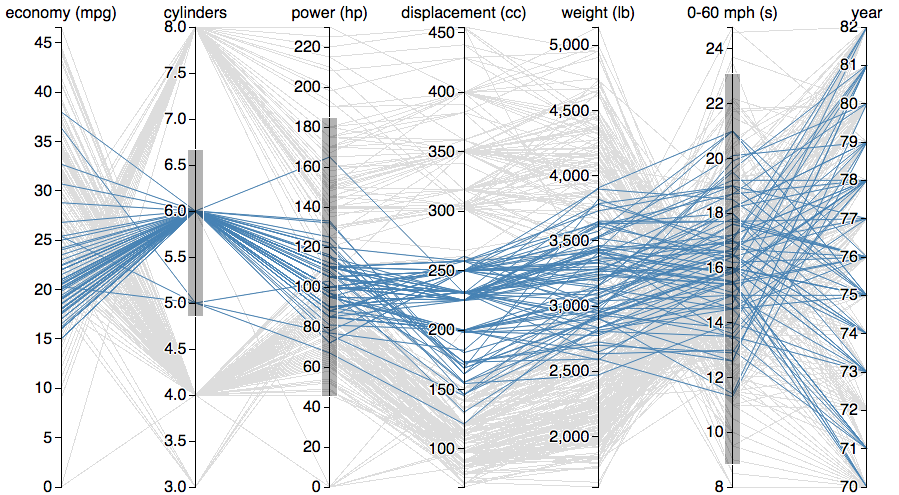
\includegraphics[width=\linewidth]{pcp}
	\caption{Direct manipulation in a parallel coordinates plot with reorder-able and brush-able axes.}
	\label{fig:lr-pcp}
\end{figure}

Another concept that can be applied to improve existing interaction techniques is \emph{fluid interaction}~\cite{Elmqvist2011}. Besides using direct manipulation as discussed previously, the interaction should produce smooth animated transitions between the state before and the state after an interaction, helping users maintain their mental maps; and provide immediate visual feedback, allowing users to know what is happening and/or what will happen next.

Typically, interaction techniques are combined to explore the data or present a known story. A classic visual information-seeking mantra by Shneiderman~\cite{Shneiderman1996} summarizes many design guidelines and interaction techniques for designing information visualizations: \emph{Overview first, zoom and filter, then details-on-demand}. With large datasets, it it challenging to create an overview and provides cues for further exploration. A more suitable approach in this case is \emph{Search, show context, expand on demand}~\cite{VanHam2009}.

\subsection{Automated Analysis Methods}
Data mining is the computational process of extracting patterns in large datasets~\cite{Tan2006}. Data mining tasks can be broadly divided into two major categories:

\begin{itemize}
		\item \emph{Descriptive tasks}. The objective is to derive patterns (correlations, trends, clusters, trajectories and anomalies) that summarizes the underlying relationships in data. Examples include cluster and association analyses. \emph{Clustering} aims to split data items to groups so that items within a group are more similar to each other than those in other groups. For example, clustering can be used to help marketers discover distinct groups of their customers before applying appropriate marketing strategies to those groups. \emph{Association} analysis discovers the connections among a set of data items. For example, it can be used to identify products that customers often purchase together such as bread and milk.
		
		\item \emph{Predictive tasks}. The objective is to predict the value of an unknown (target) attribute based on the values of other (explanatory) attributes. Examples include classification and regression. \emph{Classification} predicts discrete target variables whereas, \emph{regression} focuses on continuous ones. For example, predicting whether a customer buys a marketing product is a classification task because the target variable is binary. However, estimating a future house price is a regression task because price is a continuous-valued variable.
\end{itemize}

Next, we will discuss the clustering and classification tasks in more detail and how they are applied together with visualizations to help users gain deeper insight into the data. We also present some commonly used text mining techniques for exploring large sets of documents, which is essential in visual analytics~\cite{Thomas2005}.

\subsubsection{Clustering}

\paragraph{Overview}
Cluster analysis finds similarities between data points based on the characteristics of data attributes and groups similar data points into clusters. Clustering is regarded as \emph{unsupervised learning}~\cite{Han2011} because it can reveal hidden structure of a dataset that does not have \emph{labels} (or groups) defined. The most common clustering algorithm is \emph{k-means}~\cite{Lloyd1982}. Given a set of data points $(x_1, x_2, \dots, x_n)$, k-means clustering aims to partition them into $k$ clusters $(S_1, S_2, \dots, S_n)$, such that the within-cluster sum of squared distances is minimized: 
\[
\sum_{i=1}^k\sum_{x\in S_i} \lVert x-\mu_i \rVert^2
\]
where $\mu_i$ is the center of points (i.e., centroids) in $S_i$. 

The algorithms works as follows. Initially, partition data points into $k$ non-empty random subsets. Then, compute the centroids of the current clusters, and assign each data point to the cluster with the nearest centroid. Repeatedly recompute the centroids and reassign the cluster of each data point until no assignment can be done. This k-means clustering algorithm is efficient but often terminates at a local optimal. More detailed analysis of k-means and other clustering algorithms are out of the scope of this thesis and can be found in data mining textbooks~\cite{Tan2006,Han2011}.

\paragraph{Application Examples}
Human motion tracking data has been applied in various research fields such as medicine, sports and animation~\cite{Bernard2013}. The data consists of temporal sequences of human poses represented by a set of 3D joint positions (e.g., head, hands, elbows and knees). However, analyzing a large collection of such temporal and high-dimensional datasets is challenging. To gain an overall understanding of the data, MotionFlow~\cite{Jang2016} applies a k-means clustering method using a simple Euclidean distance of 3D joints as the similarity measurement. A cluster of human poses is represented as a glyph with a stick figure showing the centroid of the cluster and semi-transparent ghosts around the center figure for other similar poses (\autoref{fig:lr-MotionFlow}).

\begin{figure}[!htb]
	\centering
	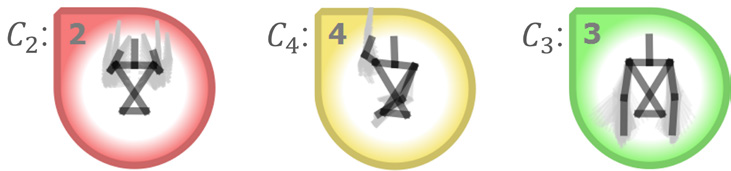
\includegraphics[width=.8\linewidth]{clus-MotionFlow}
	\caption{Visual representation of human pose clusters. \is{Jang2016}}
	\label{fig:lr-MotionFlow}
\end{figure}

MotionFlow uses a force-directed graph of clusters to illustrate their relationship with node distance mapping to the similarity of pose clusters and edges indicating the directed transition between two clusters. Edges are color coded to represent the transition frequency. A user is allowed to interactively change the number of clusters, enabling exploration of the dataset. However, the re-clustering process may change all existing clusters and make it difficult for the user to keep track. To address this issue, MotionFlow allows the user to select the clusters to be locked or unchanged during the re-clustering process. He or she is also able to interactively merge or split clusters according to his or her own assessment.

To achieve the same objective of gaining an overall understanding of human motion tracking data, MotionExplorer~\cite{Bernard2013} applies a different cluster analysis method -- hierarchical clustering~\cite{Han2011} -- which seeks to build a hierarchy of clusters. MotionExplorer takes a divisive approach considering all data items starting within the same cluster and splitting them until a termination condition is met. One of the important decisions in this clustering technique is to determine which cluster to split next. The user is allowed to choose among several splitting strategies such as \emph{maximum standard deviation} to split the most varied cluster first and \emph{highest number of elements} to split the largest cluster first. The hierarchy is visualized as a dendrogram as in \autoref{fig:lr-MotionExplorer}. Clusters are obtained by cutting the dendrogram at the desired vertical level: each connected branch forms a cluster. The vertical axis of the dendrogram can encode different variables depending on the splitting strategy. In \autoref{fig:lr-MotionExplorer}, it shows the standard deviation of each cluster and the user is allowed to slide the cutting value to adjust the resulting clusters.

\begin{figure}[!htb]
	\centering
	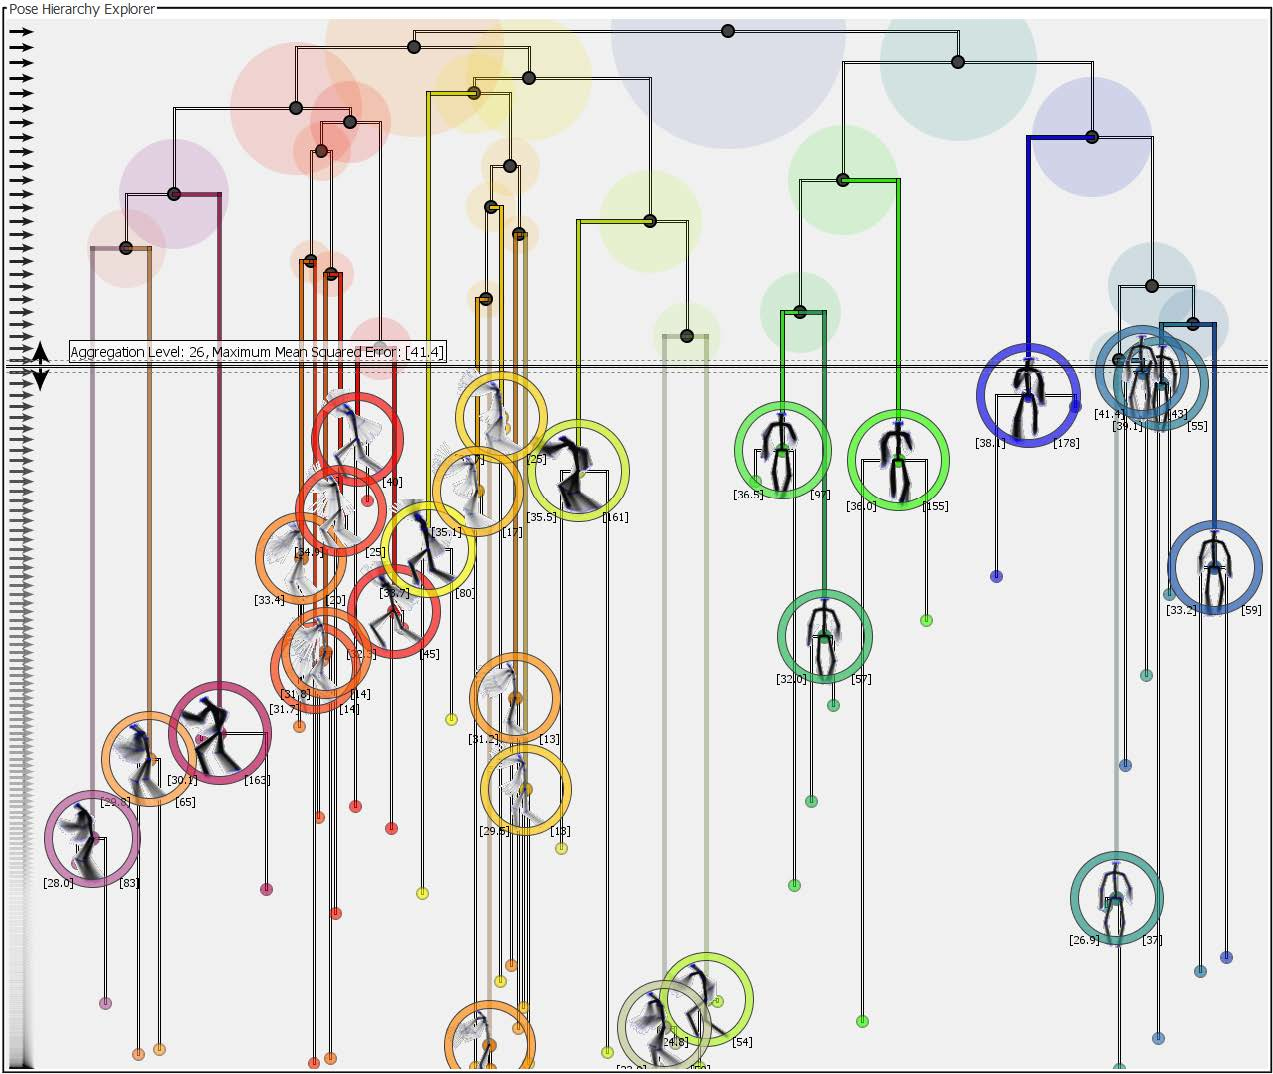
\includegraphics[width=\linewidth]{clus-MotionExplorer}
	\caption{A divisive hierarchical clustering of human poses visualized as a dendrogram. \is{Bernard2013}}
	\label{fig:lr-MotionExplorer}
\end{figure}

A different approach in hierarchical clustering is bottom-up or agglomerative clustering. The process starts with singleton clusters before merging the most similar clusters together until a termination condition is met. NewsLab~\cite{Ghoniem2007} applies such an approach in analysis of large scale broadcast news video collections. It builds a hierarchy of clusters over all keywords extracted from available video captions based on their co-occurrences in the news stories. Therefore, strongly correlated keywords are grouped into the same clusters whereas loosely related keywords are separate in different clusters. Each cluster is visualized as a stream showing the evolution of the keywords within the cluster over time with closely related clusters placed close to each other to allow navigation to different depths of the cluster hierarchy (\autoref{fig:lr-NewsLab}).

\begin{figure}[!htb]
	\centering
	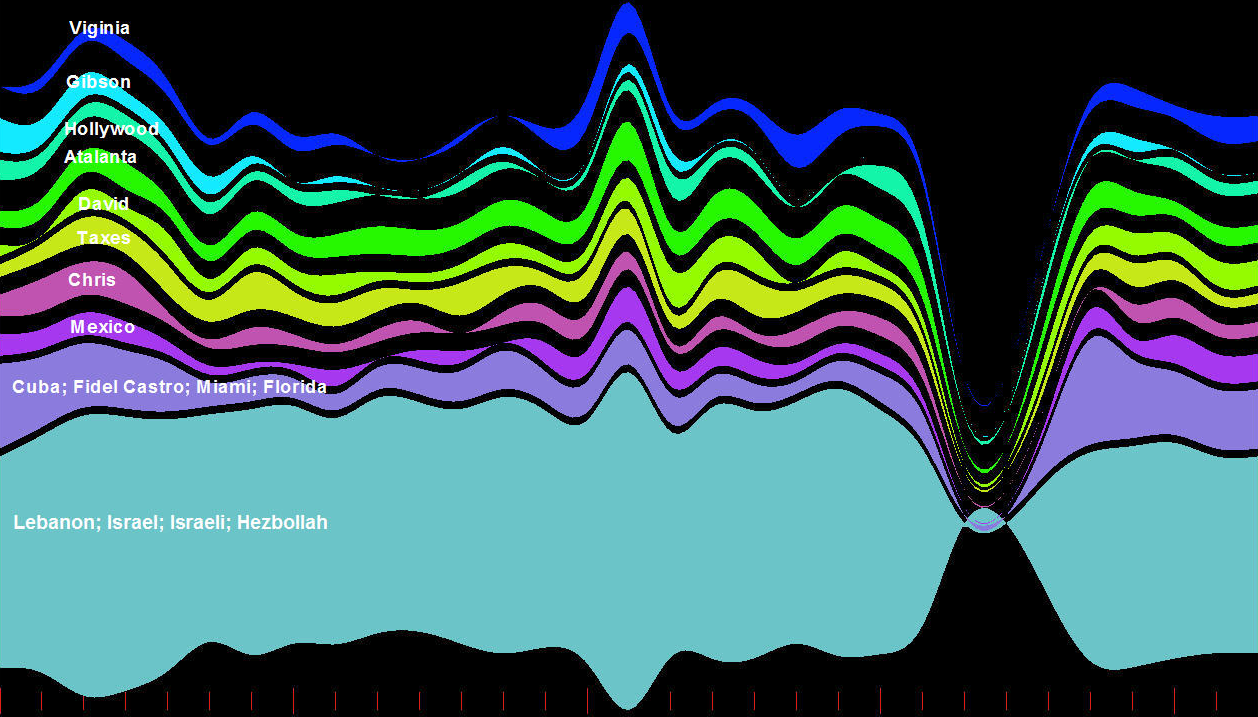
\includegraphics[width=\linewidth]{clus-NewsLab}
	\caption{An agglomerative hierarchical clustering of video captions visualized as streams. \is{Ghoniem2007}}
	\label{fig:lr-NewsLab}
\end{figure}

Understanding people movement patterns in both space and time plays an important role in urban planing. Analyzing and presenting large and complex datasets that contain a number of people in different places and their movement between those places over time are challenging. Mobility Graphs~\cite{Landesberger2016} applies cluster analysis to simplify the data in both spatial and temporal dimensions to gain an overall understanding of the datasets. First, it aggregates places using a density-based clustering technique that considers both the density of places and their flow magnitudes so that close and highly connected can be grouped together. Second, temporal aggregation groups the time steps by the similarity of those simplified places using a k-means clustering technique. \autoref{fig:lr-MobilityGraphs} shows 7 temporal clusters of simplified places. The clusters are color coded with a calendar view to reveal temporal patterns over a week. In each cluster, a node shows an aggregated place with size corresponding to the total number of people in all individual places and arrow widths representing the number of people moving between two aggregated places.

\begin{figure}[!htb]
	\centering
	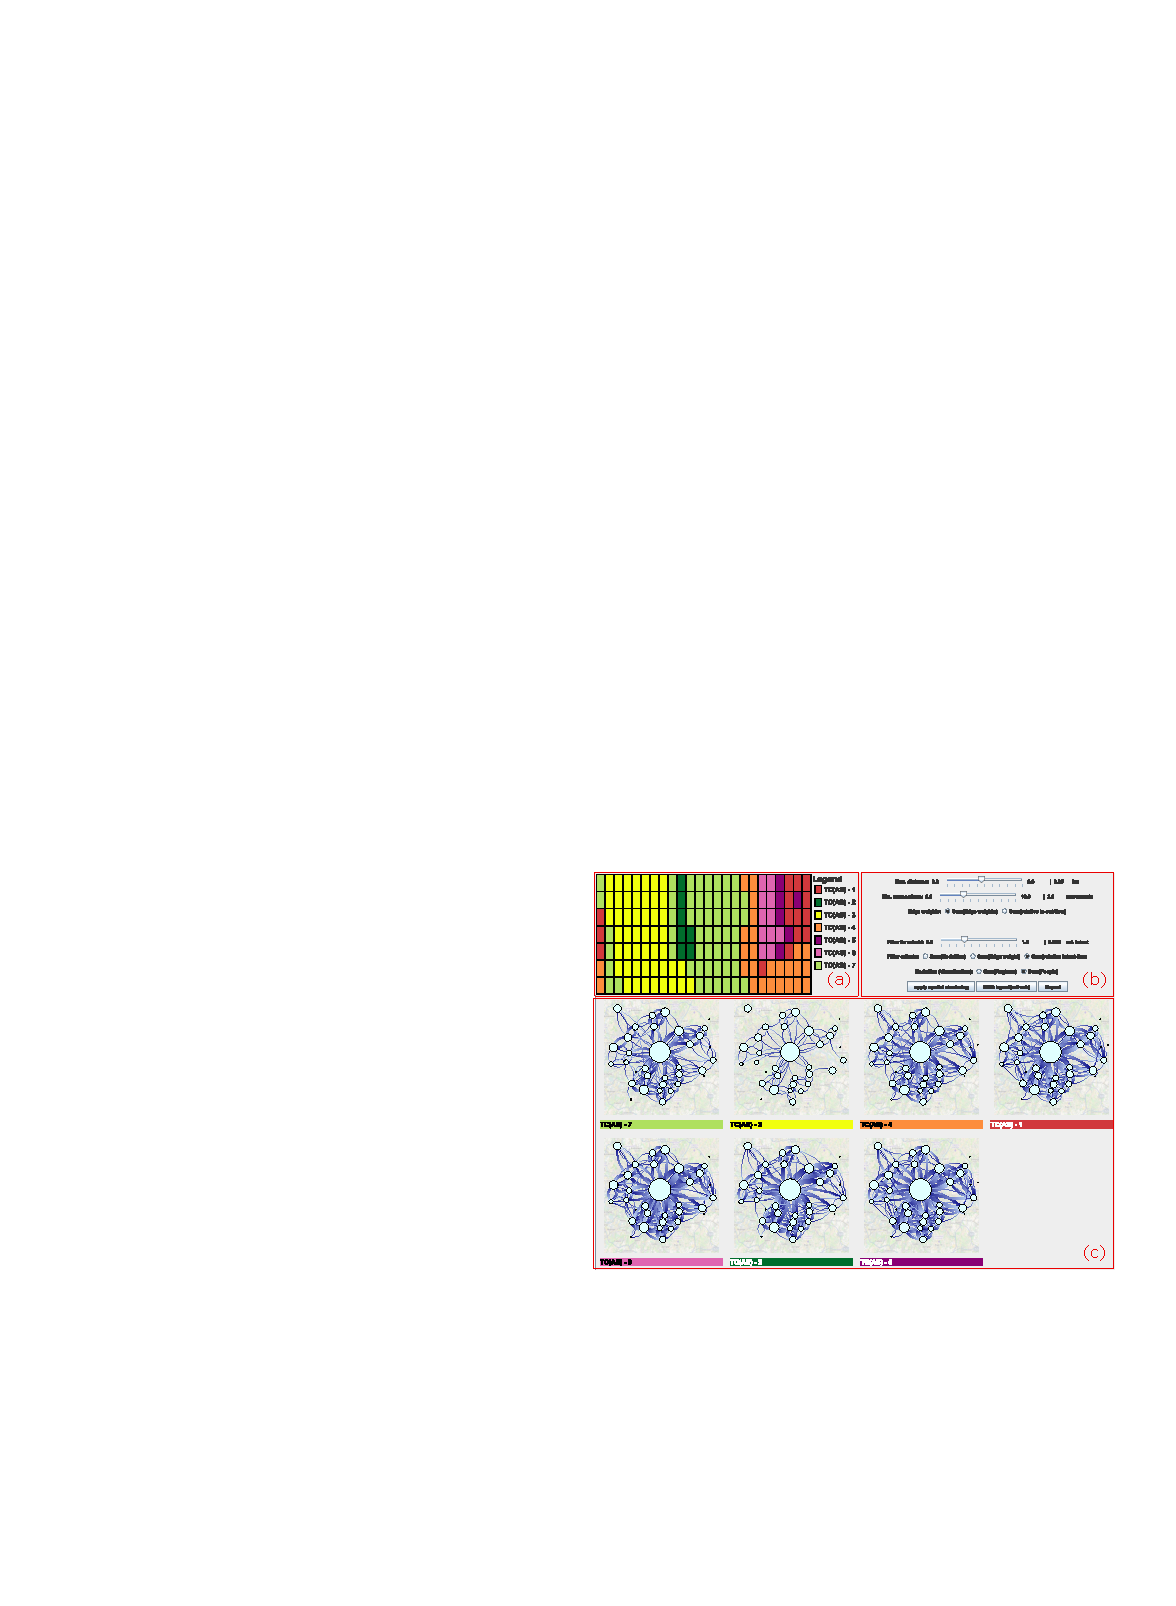
\includegraphics[width=\linewidth]{clus-MobilityGraphs}
	\caption{Temporal clusters of simplified places. \is{Landesberger2016}}
	\label{fig:lr-MobilityGraphs}
\end{figure}

\subsubsection{Classification}
\paragraph{Overview}
Classification predicts the value of a categorical (discrete or nominal) attribute based on the values of other attributes. It builds a model (or \emph{classifier}) based on a labeled training dataset (i.e., \emph{supervised learning}) and applies it in labeling new data~\cite{Han2011}. The model needs to not only identify the labels in the training dataset well but also be general enough to predict the labels of new data correctly. One common and intuitive classification algorithm is decision tree induction~\cite{Quinlan1986}. Each non-leaf node represents a ``test'' on an attribute, which splits the node to multiple branches, each for an outcome of the test. Each leaf node is associated with a class label and is the result of a sequence of tests starting from the root node.

The importance of building a decision tree is choosing which attribute to split at each node. Intuitively, we should choose attributes that can divide nodes into ``pure'' child nodes so that all data items in a child node belong to a single class and no further splits is needed. For example, in a binary classification, consider a training dataset with 10 records, 5 labeled ``true'' and 5 labeled ``false''. Attribute $A1$ splits the set to two subsets: (5 ``true'', 0 ``false'') and (0 ``true'', 5 ``false''). Attribute $A2$ splits the set to (3 ``true'', 2 ``false'') and (2 ``true'', 3 ``false''). The subsets split by $A1$ is ``purer'' than the one by $A2$ because they do not contain a mix of ``true'' and ``false''. To achieve this purity, several attribute measurements have been proposed such as \emph{information gain} and \emph{gini index}~\cite{Tan2006}. More detailed analysis of these measurements and other classification algorithms are out of the scope of this thesis and can be found in data mining textbooks~\cite{Tan2006,Han2011}.

\paragraph{Application Examples}
Exploring a large image collection, such as the set of images available on the Internet, is challenging. Besides the low-level visual features, the semantic contents of images are also effective in searching for relevant ones. Image classification techniques can be used to extract such semantic contents. For example, Fan~et~al.~\cite{Fan2004} detect salient objects in images and associate them with predefined semantic contents according to their perceptual properties. Similar contents are then grouped into a higher level semantic concept; for instance, ``sand field'', ``sea water'' and ``boat'' salient objects construct the concept of ``sea world''. Visualization can help make the output of classification algorithms more interpretable and interactive. To provide an overview of an image collection, Yang~et~al.~\cite{Yang2006} shows the extracted semantic contents, with each as a glyph, in a 2D display so that related contents are located close together using a multidimensional dimension scaling method~\cite{Borg2005}. Similarly, images are also displayed based on their similarity as in \autoref{fig:lr-SIBa}. Zooming and panning are provided to make the visualization more scalable. When an image is selected, the visualization can be switched to a \emph{rainfall} mode, in which the selected image is shown at the bottom and related images are stacked above it based on their similarity with the selected one (\autoref{fig:lr-SIBb}). Users are allowed to reassign the contents computed for each image; however, the model does not take into account the changes to improve its accuracy when classifying new images.

\begin{figure}[!htb]
\centering
\subcaptionbox{Multidimensional dimension scaling view of images.\label{fig:lr-SIBa}}{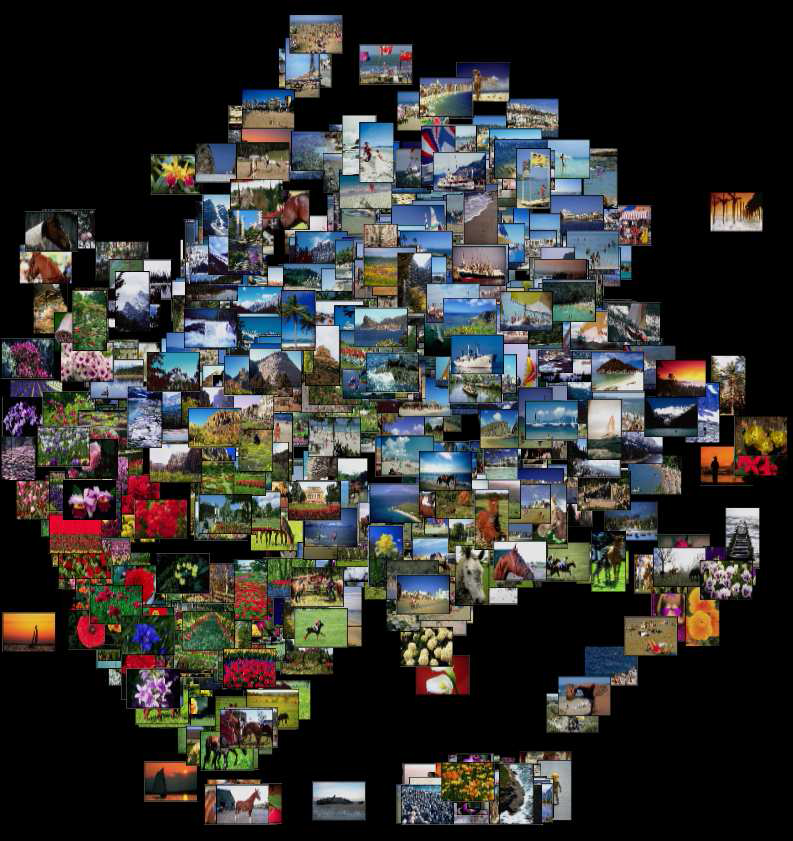
\includegraphics[height=.5\columnwidth]{clas-SIBa}} 
\hfill
\subcaptionbox{Rainfall view of a selected image with highly related images at the bottom.\label{fig:lr-SIBb}}{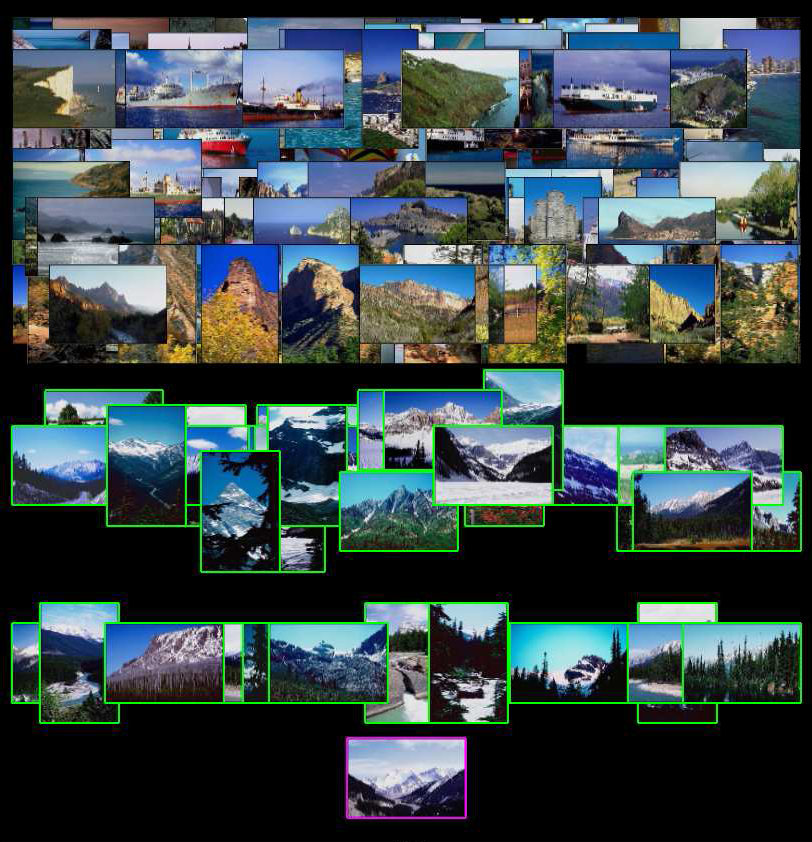
\includegraphics[height=.5\columnwidth]{clas-SIBb}} 
\label{fig:lr-SIB}
\caption{Semantic image browser. \is{Yang2006}}
\end{figure}

In a binary classification, the classifier output is either \emph{positive} or \emph{negative}. Two types of error can happen include \emph{false positive} (classified as positive but the actual class is negative) and \emph{false negative} (classified as negative but the actual class is positive). Depending on a domain, the costs of these error types might be considerably different. For example, wrong prediction of a healthy patient with a cancer has a much lower impact than missing a patient with a real cancer. Migut and Worring~\cite{Migut2010} allow users to adjust the trade-off between these two error types through the visualization of the classification model. Typically, a receiver operating characteristic curve~\cite{Fawcett2006} is used to illustrate the performance of a binary classifier as its discrimination threshold is varied. The curve is composed from a set of true positive rate and false positive rate pairs at various threshold values. Migut and Worring~\cite{Migut2010} replace the true positive rate with the false negative rate (\autoref{fig:lr-Migut1}) because their focus is comparing trade-off between the two error rates. Numerical data is visualized in a scatter plot with the decision boundary separating a 2D plane into two regions, each for a class (\autoref{fig:lr-Migut2}). For each data point, color shows the original class and size indicates the accuracy of the classified class. The current classification setting is shown as a red point on the performance curve, and the user is allowed to move that point along the curve to change the false positive and false negative rates. The classification reruns with the new threshold and rates and updates on the data scatter plot.

\begin{figure}[!htb]
\centering
\subcaptionbox{Performance curve of the classification model with horizontal axis showing the false positive rate and vertical axis showing the false negative rate. rates.\label{fig:lr-Migut1}}[\columnwidth]{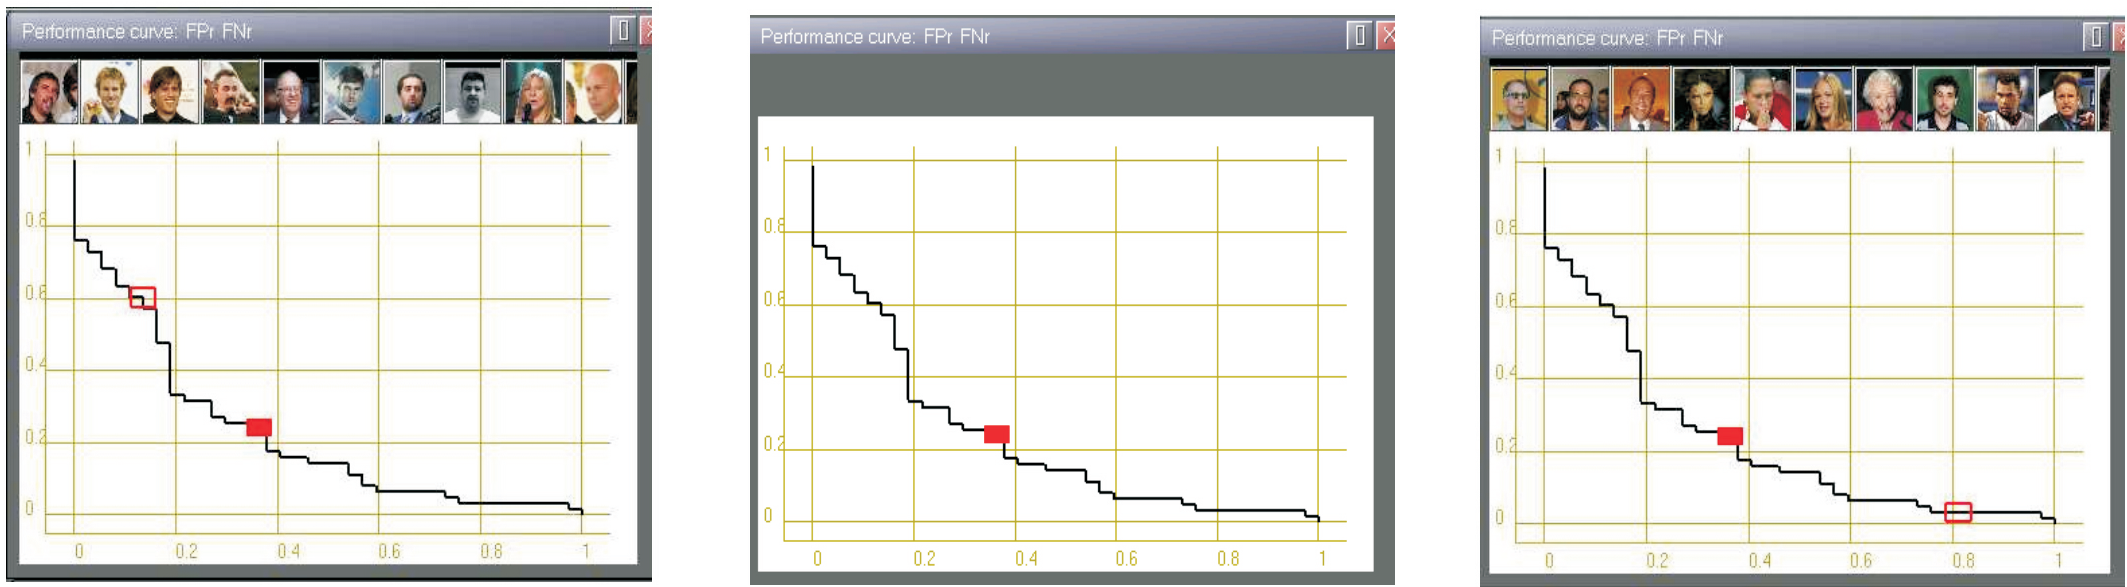
\includegraphics[width=\columnwidth]{clas-Migut1}} 
\\
\subcaptionbox{Data with color indicating original class and size showing classification accuracy.\label{fig:lr-Migut2}}[\columnwidth]{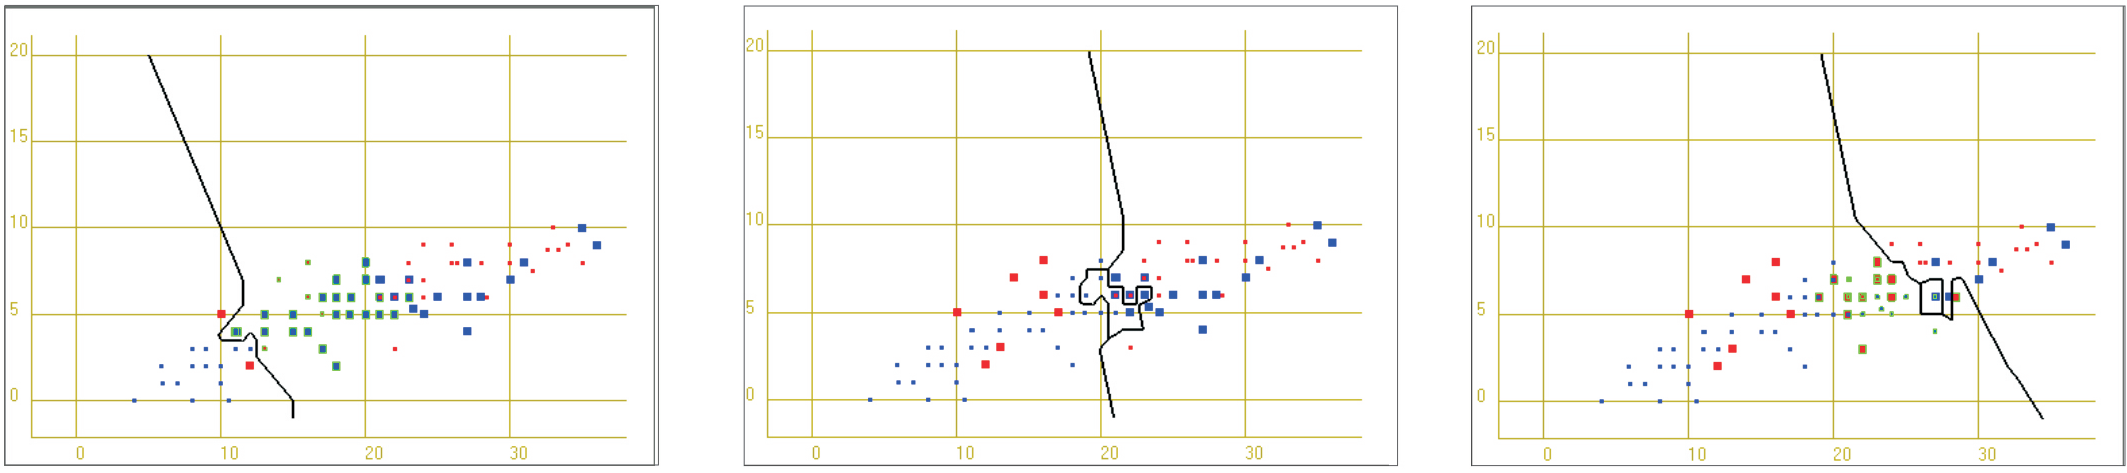
\includegraphics[width=\columnwidth]{clas-Migut2}}
\caption{Visualization and interaction of a classification model. Figure in the middle shows the initial state of the system, with initial operating point on the performance curve and corresponding data scatter plot. Figure on the left shows the state of the system when an expert manipulates the operating point to include more false negatives and on the right to include more false positives. \is{Migut2010}}
\end{figure}

Classification requires training data; however, it can be time-consuming and laborious to produce such a dataset. ScatterBlogs2 includes an interactive classifier that speed up the training data labeling and classifier construction before applying it in real-time monitoring messages of interest~\cite{Bosch2013}. First, the user can search for relevant messages using a standard keyword query. The system then highlights non-trivial terms that frequently co-occur with the original keywords. The result set of highly relevant messages can be used as \emph{positive} samples, whereas some arbitrary messages not returned in the result set can be used as \emph{negative} ones. After creating an initial classifier, the user can inspect messages to correct and update the classifier through the message visualization. Messages are shown in a map as a colored glyph with color hue indicating class and brightness showing classification confidence (\autoref{fig:lr-ScatterBlogs2}). Messages can be filtered by confidence, allowing the user to focus on ones with less certainty, which need human expert to verify. To further speed up the classifier creation, ScatterBlogs2 offers self-training, a technique that iteratively uses messages classified with the highest confidence as labeled data. 

\begin{figure}[!htb]
	\centering
	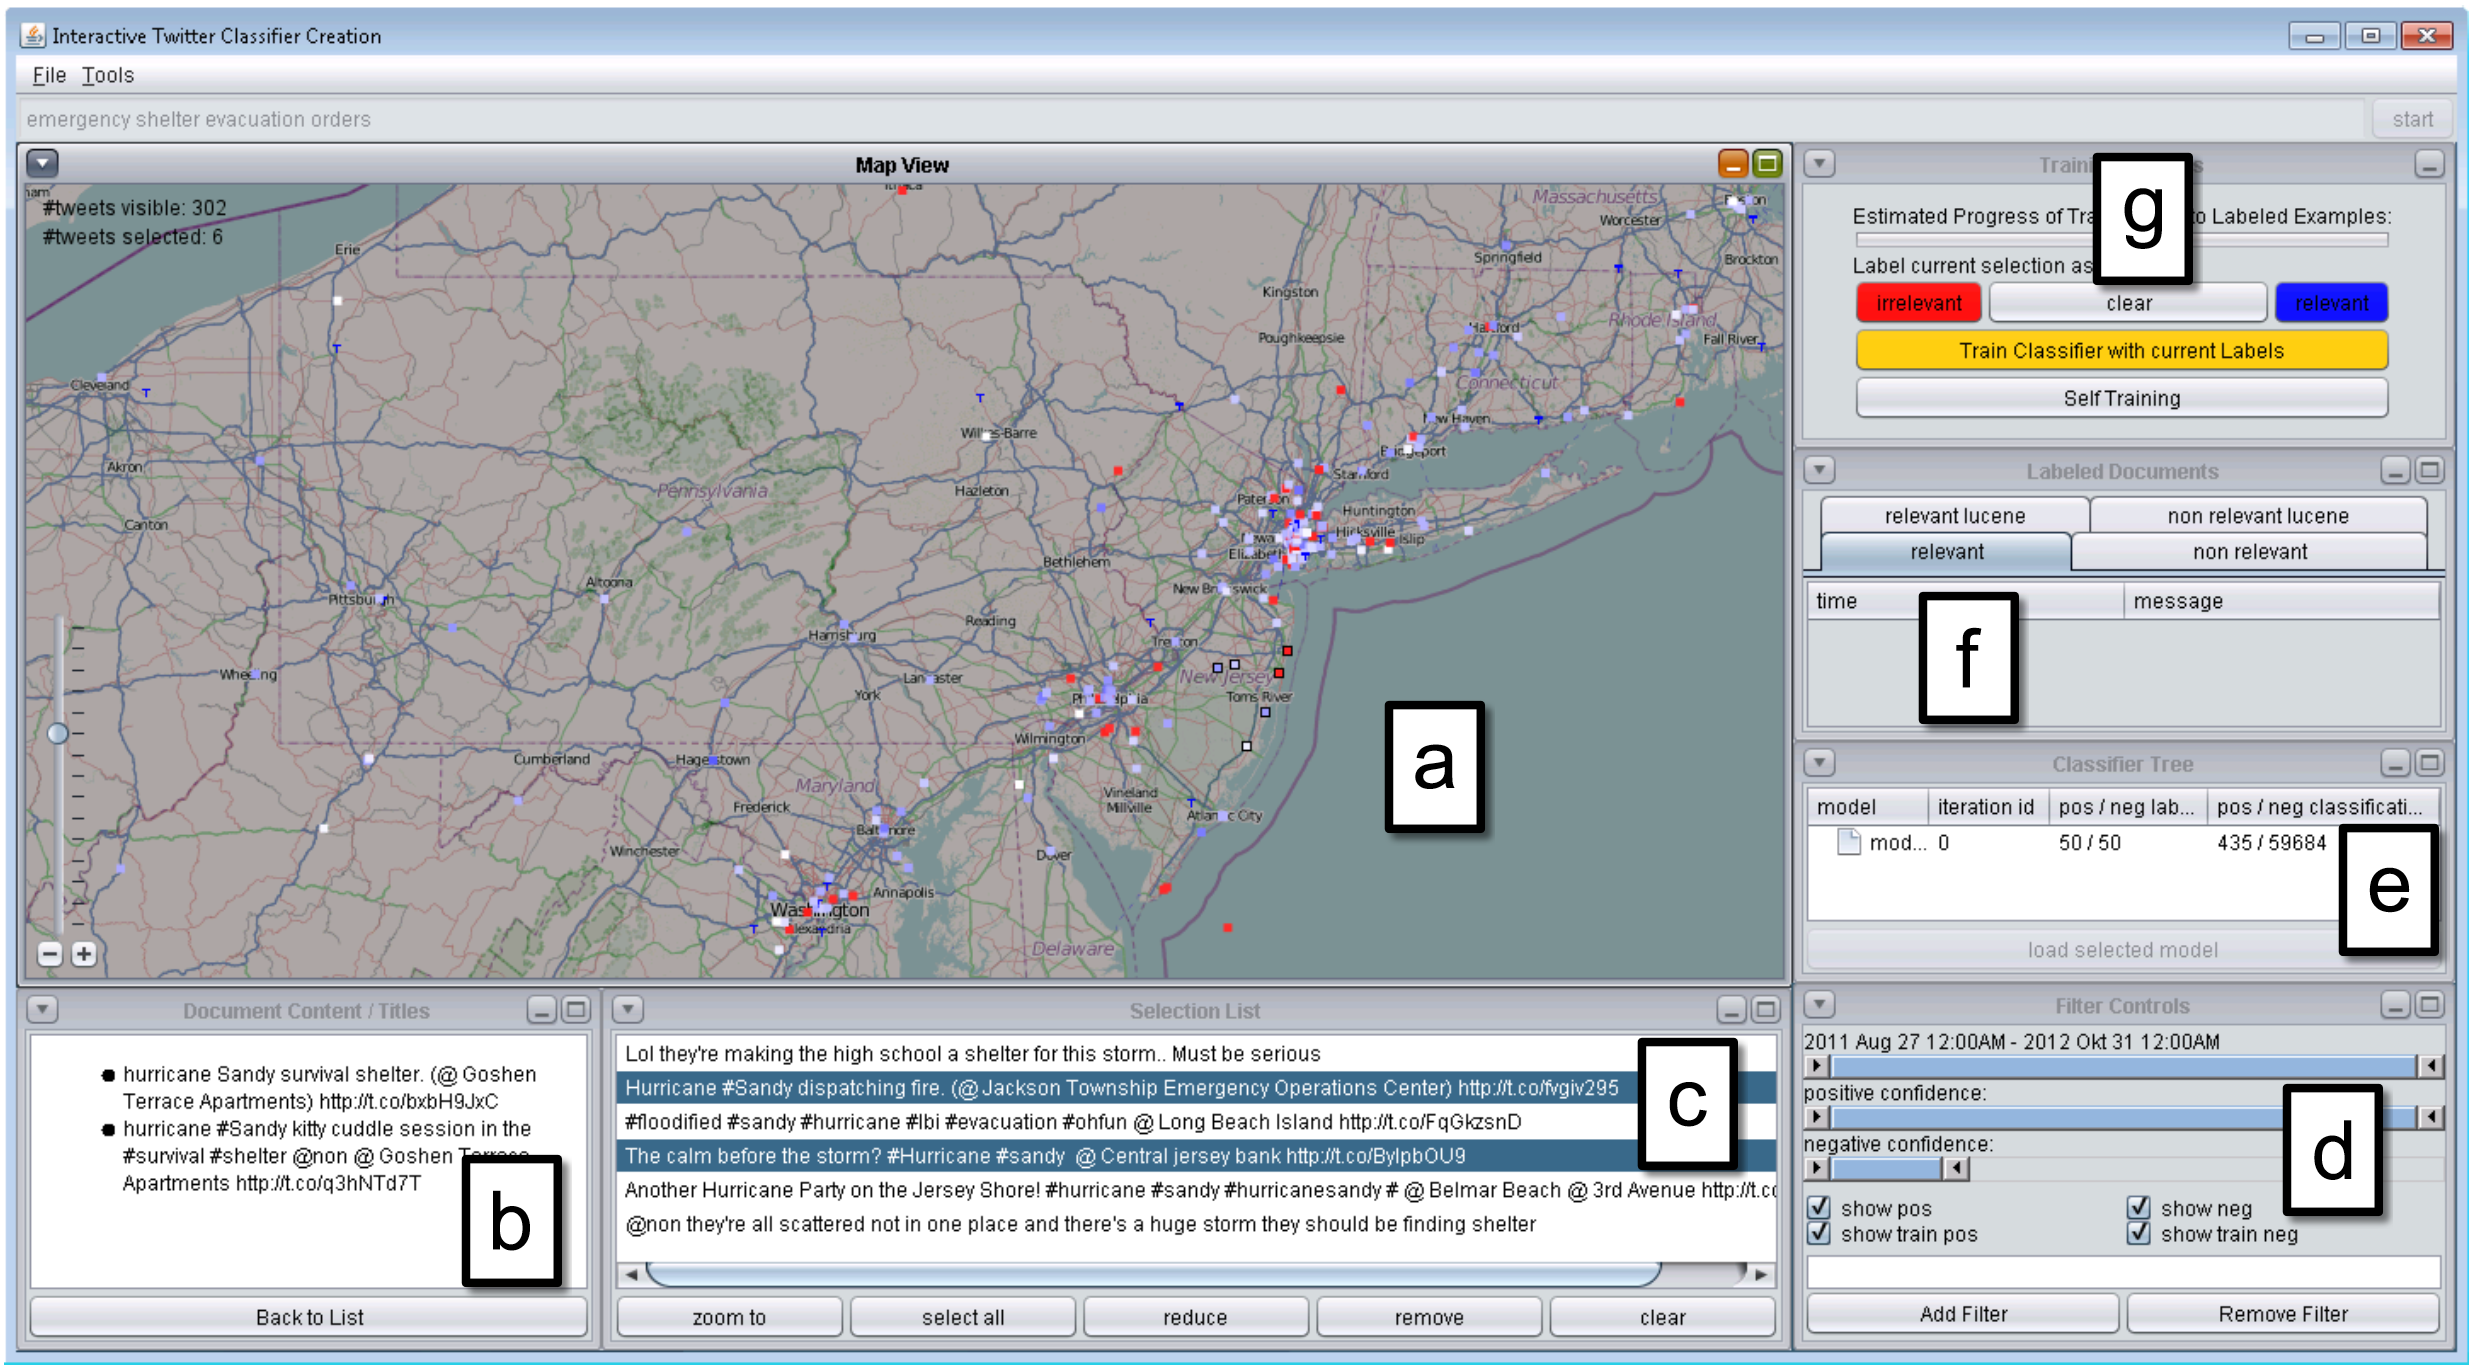
\includegraphics[width=\linewidth]{clas-ScatterBlogs2}
	\caption{The classifier creation environment of ScatterBlogs2. \is{Bosch2013}}
	\label{fig:lr-ScatterBlogs2}
\end{figure}

An essential step in classification of high dimensional datasets is feature selection, which selects a subset of relevant features for use in model construction without much loss of information. This step also simplifies the model and reduces training time. INFUSE~\cite{Krause2014} supports users to explore the predictive power of features in their models. The system allows comparison of features across four feature selection algorithms. Each feature is shown as a circle glyph divided into four equal quadrants, each for an algorithm (\autoref{fig:lr-INFUSE}). A quadrant is further split into 10 slices, each for a cross-validation fold (or random subset of data) to ensure the result  robust. The length of a slice indicates the rank of that feature using a given algorithm. Therefore a glyph can show how its feature performs in different algorithms. To have an overview of all features, INFUSE shows multiple glyphs in either a sequential layout or a scatter plot, where different options can be used for axes such as average rank of a feature or a more sophisticated importance measurement. It also allows users to explore four classification algorithms by showing the score of all 16 combination of feature selection and classification algorithms. More importantly, users are allowed to build their own model by selecting features besides the ones produced by the four given algorithms. The custom feature set is then included in the classification score comparison.

\begin{figure}[!htb]
	\centering
	\includegraphics[width=\linewidth]{clas-INFUSE}
	\caption{The feature glyph in INFUSE. \is{Krause2014}}
	\label{fig:lr-INFUSE}
\end{figure}

\subsection{Evaluation Methods}
A visualization, no matter how novel and interesting it is, needs to be evaluated to check whether it meets the design goals and supports the target users to complete the intended tasks. Evaluation has been a research topic in visualization when the field becomes more matured~\cite{Plaisant2004}. Excellent reviews of visualization evaluation with different perspectives include evaluation techniques~\cite{Carpendale2008}, scenarios~\cite{Lam2012} and design process~\cite{Munroe2009}.

In this section, we review the evaluation techniques based on the visualization design model by Munzner~\cite{Munroe2009}, helping address different concerns separately. The four levels include: explain the tasks and available data in the vocabulary of the problem domain, abstract them into domain-independent operations and data types, design visual encoding and interaction techniques to solve the abstract tasks, and develop algorithms to execute these techniques efficiently. Each level has its own \emph{threats} to validity and methods to address them. Two types of methods are distinguished: \emph{immediate} approaches can be done before inner levels are implemented, whereas \emph{downstream} approaches requires all inner levels are completed. The threats and evaluation methods are summarized in \autoref{fig:lr-nested-model}.

\begin{figure}[!htb]
	\centering
	\includegraphics{nested-model}
	\caption{Threats and validation at each of the four nested levels of visualization design. \is{Munzner2014}}
	\label{fig:lr-nested-model}
\end{figure}

\subsubsection{Domain Problem and Data Characterization}
The domain problem of target users is investigated to see if visualization is a potential solution. The primary threat is that the problem is mischaracterized: the users do not really suffer from the identified problem. An immediate form of validation is \emph{field study}~\cite{Carpendale2008}, where the investigator observes how target users act in real-world settings in order to learn and verify the characterization. Another technique is \emph{contextual inquiry}~\cite{Holtzblatt1993}, which allows the investigator to occasionally interview while the user is engaged in the process. One example is the study by Sedlmair~et~al.~\cite{Sedlmair2008} on current working behavior and environments of analysis and diagnosis experts in the automotive industry.

One downstream form of validation is to report the rate the adoption rate of the tool by the target users. High effort is required to make the visualization solution reliable and deployable in the real-world environment. Examples include a field study of Google's Notebook product~\cite{Russell2008} and 6-week field trial of SparTag.us -- a tagging system for foraging web content~\cite{Hong2008}.

\subsubsection{Operation and Data Type Abstraction}
The threat at this level is the identified data and task abstraction do not solve the characterized problem. Only downstream approaches can be used to validate the abstraction. The deployed system needs to be used by target users completing their routine tasks in real-world environment. The goal of this evaluation is to collect anecdotal evidence that the solution is in fact useful. The observation and interview need to focus on understanding how the tool is used, and how it helps or hinders the users in performing their tasks. An example is a longitudinal field study of LiveRAC system that supports analysis of system management time-series data~\cite{McLachlan2008}.

Evaluating the visualizations for supporting sensemaking can be done at this level, as the \emph{evaluating visual data analysis and reasoning} scenario in the taxonomy by Lam~et~al.~\cite{Lam2012}. Due to the nature of sensemaking, evaluation is often carried out as case studies~\cite{Kang2011} with observation and interview, and followed by qualitative data analysis~\cite{Lazar2010}. Attempts also have been made to quantify the insight or knowledge gained during sensemaking~\cite{Wilson2013}.

\subsubsection{Visual Encoding and Interaction Design}
At the design level, the threat is the chosen design is ineffective at communicating the desired abstraction to the user. One immediate form of validation is to justify every design decision based on known design principles such as the ones discussed in \autoref{sub:lr-design}, or more comprehensive predefined guidelines as in heuristic evaluation~\cite{Zuk2006}. Asking experts to review the design prototype also provides valuable feedback~\cite{Tory2005}.

A common downstream approach is to conduct a controlled experiment comparing the design with other state-of-the-art alternatives~\cite{Xu2012}. A number of participants, depending on the  expected size of the experiment, carry out a number of tasks representing real-world cases. Typically, task completion time and accuracy are measured and analyzed using hypothesis testing methods~\cite{Field2003}. Post-task interviews are often combined to establish deeper understanding about how the visualization is used. If the experiment can be completed online, crowd-sourcing approach using Amazon's Mechanical Turk service can help largely increase the size of participants~\cite{Heer2010a}. Another downstream approach is the measurement of common aesthetic metrics such as the number of edge crossings and edge bends that have been used in graph visualization~\cite{Sugiyama1981}.

\subsubsection{Algorithm Design}
The primary threat at this level is the algorithm is suboptimal in terms of time or memory performance. In interactive visualization, it is essential to ensure the interaction responsive in real-time. Analyzing the complexity of the algorithm using the standard approaches from the computer science literature~\cite{Cormen2009} is an intermediate form of validation. The complexity can be computed based on the size of dataset or the display screen. Downstream approaches include measuring running time and memory usage for benchmark datasets.

%http://www.cc.gatech.edu/~stasko/papers/vast09-eval.pdf
%https://www.purdue.edu/discoverypark/vaccine/assets/pdfs/publications/pdf/Beyond%20Usability.pdf
%http://www.cc.gatech.edu/~stasko/7450/Papers/fekete08.pdf
%https://www.cs.ubc.ca/~tmm/courses/cpsc533c-05-fall/readings/vov.pdf
%\section{Provenance}
todo: different of data and analytic provenance.Provenance in ordinary context, give examples (food, art)
where?
%must read: very releveant: http://www.cc.gatech.edu/~aendert3/resources/ragan-vast-2015.pdf
\subsection{Data Provenance}
Data provenance research has been taken in different fields, notably scientific workflows and databases. Scientific experiments may consist of thousands of steps, with each step involving distributed data sources and computational data models~\cite{Gil2007}. Workflows have been used to facilitate the assembly, automation and management of such experiments. Notable scientific workflow systems with provenance enabled include Tarvena~\cite{Zhao2008}, Kepler~\cite{Bowers2006} and VisTrails~\cite{Bavoil2005}. Provenance plays an important role in scientific workflows, aiming to support data interpretation, reproduction of experiment results, troubleshooting and optimization~\cite{Miles2007}. The provenance of long and complex workflows is huge, thus pose challenges in storing, querying, and making sense of such data~\cite{Davidson2007}.

Curated databases are populated and updated with a great deal of human effort, typically published on the web~\cite{Buneman2008}. A well-known example is Wikipedia -- a free Internet encyclopedia that allows its users to edit almost any article accessible. Each record in these databases, such as a Wikipedia article, may be edited by many users and referred to other internal and external sources. This produces problems in attribution and provenance: who edited what at when. Research in database provenance can be characterized into a why-where-how framework~\cite{Cheney2007}. \emph{Why}-provenance focuses on the lineage of the output: for each tuple $t$ in the output, the lineage of $t$ is a set of tuples in the input data that helps produce $t$~\cite{Cui2000}. \emph{How}-provenance concerns how the output tuple $t$ is derived from the query~\cite{Green2007}. Finally, \emph{where}-provenance describes specific locations, or cells in relational databases, of the input data that contribute to the query output~\cite{Buneman2001}. To compute these types of provenance, two general approaches have been introduced~\cite{Buneman2008}. An \emph{eager} approach adjusts the query to pass the extra provenance information to the output. Whereas, a \emph{lazy} approach computes provenance on demand.

Data provenance research in scientific workflows and databases has mainly focused on closed systems, which have full access to the data and its provenance. Modern applications with service-oriented~\cite{Papazoglou2007} and cloud-computing~\cite{Buyya2009} architectures bring challenges in tracking and exchanging provenance information across systems. The \emph{Open Provenance Model} is designed to address these challenges~\cite{Moreau2011}. It also supports a digital representation of provenance for any ``thing'', whether produced by computer systems or not. Three types of objects are defined in the model for building this representation. An \emph{artifact} is a state that can be a digital or physical object. A \emph{process} is a series of actions performed on or caused by artifacts, and resulting in new artifacts. An \emph{agent} acts as a catalyst of a process, managing its execution. Different types of causal relationships can be added between these nodes, forming a \emph{provenance graph} as shown in \autoref{fig:lr-provenance-graph}.

\begin{figure}[!htb]
	\centering
	\includegraphics[width=\linewidth]{provenance-graph}
	\caption{A provenance graph for ``cake baking'' using the Open Provenance Model. The cake (artifact) was baked (the process) by John (the agent) using ingredients including butter, eggs, flour and sugar (artifacts). \is{Moreau2011}}
	\label{fig:lr-provenance-graph}
\end{figure}

The Open Provenance Model is general and can be extended in both the structure and vocabulary to represent domain-specific problems. ProveML~\cite{Walker2013} is an extension of this model for recording the provenance of data, analytical process and interpretations in human terrain visual analytics.

\subsection{Analytic Provenance}
Definition from ~\cite{North2011}, our agenda~\cite{Xu2015}

\subsubsection{Model}
Modeling of analytic provenance: 4-level model by Gotz and Zhou and other vis task/action taxonomies such as classic Shneiderman's task by data type~\cite{Shneiderman1996}, Amar's low-level~\cite{Amar2005}, Amar's high-level~\cite{Amar2004}, more recent Bhemer's typology what-why-how~\cite{Brehmer2013}.

\subsubsection{Capture}
combine previous reviews from the draft survey of analytic provenance, research agenda, and capture in the context of online sensenmaking the last paper
%\section{Visualization of Provenance Data}
We characterize the visualization of provenance data based on the level of semantics involved in the collected data~\cite{Gotz2009}, including event, action, sub-task and task. Because low-level events contain little semantics, they are often visualized and analyzed after users finished their tasks in order to gain deeper understanding about their processes rather than to provide near real-time sensemaking support to the users during their tasks. For example, visualization of users' mouse clicks can reveal patterns of application usage~\cite{Matejka2013} and highlight some important usability issues, such as pages where users spent a lot of time and pages where they got lost during the task~\cite{Waterson2002}. User interactions with visual analytics systems can be visually examined to recover their reasoning processes employed in their analysis tasks such as specific findings they found and strategies they used~\cite{Dou2009, Guo2016}. Interaction logs have also been used to predict user performance of basic visualization tasks like visual search~\cite{Brown2014}.

Next, we focus on the visualization of levels with richer semantics. Actions and states
(the visualization results of the actions) are commonly used to show the analysis process. Sub-tasks and tasks are often documented by users in a graphical reasoning process.

\subsection{Visualizing the Analysis Process}

\subsubsection{Visual Representation}

\paragraph{Text}
Text is commonly used to describe actions or states, such as names of actions, titles of visited web pages and content of user notes. Text can provide accurate information, but long text makes it difficult for users to understand and recognize. A graphical browser history by Ayers and Stasko~\cite{Ayers1995} shortens web page titles to accommodate more pages in the view. Within a given width, its algorithm preserves complete words at both ends of the title and trims characters in the middle if necessary. Kaasten, Greenberg and Edwards~\cite{Kaasten2001} compare the recognizability of titles between various string sizes for all three truncation methods (text is truncated at the beginning, middle or end of the title). The results show that for medium (60\%) recognition, we need 15--20 letters (depending on
the truncation method) for web sites, and 28--39 letters for
exact pages. For longer text such as user notes, machine learning techniques for text summarization could be beneficial~\cite{Nenkova2012}.

\paragraph{Icon}
Sensemaking actions can be represented by graphical symbols, allowing users to easily distinguish them. They can be used alone to represent the analysis process when the visual result of each action is out of interest (\autoref{fig:lr-action-1}). Alternatively, these icons can be used together with interface states, connecting the one before and the one after an action (\autoref{fig:lr-action-2}).

\begin{figure}[!htb]
\centering
\subcaptionbox{A sequence of icons displaying the analysis process. \is{Gotz2009}\label{fig:lr-action-1}}{\includegraphics[width=.8\columnwidth]{action-1}}

\vspace{.5\baselineskip}

\subcaptionbox{Iconic actions connecting two visualization states. \is{Ma1999}\label{fig:lr-action-2}}{\includegraphics[width=.8\columnwidth]{action-2}}
\caption{Using icons for representing actions.}
\end{figure}


\paragraph{Thumbnail}
Thumbnails are commonly used to represent visualization states, aiding users' recognition of previous ones. One study suggests that a thumbnail size of 96 pixels square could provide 60\% accurate recognition of a visited web site~\cite{Kaasten2001}. For the same accuracy but in recognizing an exact web page, the thumbnail size rises to 144 pixels square. Additional information can be added to a web thumbnail to improve its recognition such as how often the represented page is revisited and whether that page is bookmarked or not~\cite{Cockburn1999}. For visualization thumbnails, visual encodings and parameters that were used to produce the visualization can also be embedded (\autoref{fig:lr-thumbnail-encoding}), providing more provenance information to the users.

\begin{figure}[!htb]
	\centering
	\includegraphics[width=\columnwidth]{thumbnail-encoding}
	\caption{Visualization thumbnails with additional information about any filtering used, the characteristics of the filtered subset of data and the visual encoding. \is{Walker2013}}
	\label{fig:lr-thumbnail-encoding}
\end{figure}

It may be necessary to apply pre- and post-processing adjustments to make the visualization thumbnails more recognizable~\cite{Heer2008}. For example, high-frequency visual elements that are not helpful in a small size such as gridlines and element borders can be removed to prevent their domination in the resulting thumbnail. As a result of down-sampling techniques, colors of data items may be different from them in the original visualization. Therefore, readjusting the color to match its intended value could help users to recognize the visualizations they analyzed in the past.

The default snapshot may also be an imperfect representation of a web page, especially if it contains a lot of text. Teevan~et~al.~\cite{Teevan2009} propose an automatic method to produce a thumbnail improving its recognition. It consists of three components: some salient text at the top-left hand corner, a salient image below the text, and a watermarked logo superimposed at the bottom left hand corner of the image. The salient text contains about 20 first characters of the web page title. The salient image and the branding logo are chosen from the page using machine learning. \autoref{fig:lr-enhanced-thumbnail} shows such a thumbnail.

\begin{figure}[!htb]
	\centering
	\includegraphics{enhanced-thumbnail}
	\caption{An enhanced web thumbnail (right) as a composite of some salient text, a salient image and a branding logo. \is{Teevan2009}}
	\label{fig:lr-enhanced-thumbnail}
\end{figure}

Besides recognizing previous states, seeing the difference between a state and the one before it is also important in understanding the analysis process. One approach is to highlight the difference between two consecutive states (\autoref{fig:lr-state-2}). The changes may only happen at one small portion of the entire interface. Therefore, showing only that area in both states could help users quickly identify the difference (\autoref{fig:lr-state-3}).

\begin{figure}[!htb]
\centering
\subcaptionbox{Modified items are highlighted with green borders. \is{Klemmer2002}\label{fig:lr-state-2}}[.47\columnwidth]{\includegraphics[height=.33\columnwidth]{state-2}} 
\hfill
\subcaptionbox{Changed area is cropped and shown in both  states. \is{Kurlander1988}\label{fig:lr-state-3}}[.47\columnwidth]{\includegraphics[height=.33\columnwidth]{state-3}}
\caption{Techniques improving recognition of state changes.}
\end{figure}

\subsubsection{Layout}

\paragraph{Linear Layout}
Provenance data usually contains an inherent \emph{time} attribute, recording when an action happened. An approach that emphasizes on the order of completed actions is to show them as a linear sequence of items like a comic strip~\cite{Kurlander1988,Meng1998}. This layout facilitates visual scanning of past actions, allowing users to quickly understand the analysis process. \autoref{fig:lr-comic-strip} shows such a layout.

\begin{figure}[!htb]
	\centering
	\includegraphics[width=\columnwidth]{comic-strip}
	\caption{Comic strip layout. A sequence of past actions in chronological order. \is{Heer2008}}
	\label{fig:lr-comic-strip}
\end{figure}

If the absolute timestamps of actions are of interest, a continuous timeline~\cite{Derthick2001} is a more suitable layout. Actions are positioned along the time axis at when they happen (\autoref{fig:lr-continuous-timeline-1}) or during which they last (\autoref{fig:lr-continuous-timeline-2}). The time axis can be either horizontal or vertical~\cite{SandboxTimeline2012}. The layout algorithms found in these provenance timelines are quite naive. POLESTAR~\cite{Pioch2006} and the timeline from Jigsaw~\cite{Liu2010} require manual rearrangement of the events from users to solve the overlapping problem. The timeline from nSpace2 Sandbox~\cite{SandboxTimeline2012} shows events at the exact time when they happen without considering possible intersection between of them.

\begin{figure}[!htb]
\centering
\subcaptionbox{Time-point provenance data. User annotations are positioned along a time axis at when their associated events happen. \is{Gotz2006}\label{fig:lr-continuous-timeline-1}}{\includegraphics[width=\columnwidth]{continuous-timeline-1}}

\vspace{.5\baselineskip}

\subcaptionbox{Interval provenance data. User actions are shown as horizontal bars a long a time axis covering their durations. \is{Plaisant1999}\label{fig:lr-continuous-timeline-2}}{\includegraphics[width=\columnwidth]{continuous-timeline-2}}
\caption{Timeline layout for visualizing the analysis process.}
\end{figure}

Another approach is to use both the horizontal and vertical axes to represent time. BrowseLine~\cite{Hoeber2009} uses the vertical axis for \emph{macro-time} and the horizontal axis for \emph{micro-time}, similar to stem-and-leaf plots. More specifically, a two-dimensional timeline (\autoref{fig:lr-timeline-2d}) is divided into rows, each for a big time-slot, such as one hour. In each row, events happening within that hour are positioned along the horizontal axis without considering their absolute timestamps. This design assumes that users may only remember roughly when events happen, thus absolute positioning in the vertical axis facilitate them in recognizing past events. Moreover, relative positioning in the horizontal axis could help pack more events and prevent overlapping.

\begin{figure}[!htb]
	\centering
	\includegraphics[width=\columnwidth]{timeline-2d}
	\caption{2D timeline. The vertical axis represents macro-time, whereas the horizontal axis represents micro-time. Events within a macro time-slot are positioned in chronological order as a comic strip. \is{Hoeber2009}}
	\label{fig:lr-timeline-2d}
\end{figure}

\paragraph{Branching Layout}
Many sensemaking systems allow users to revisit their past states such as through undo/redo features or backward/forward in web browsers. From a past state, if the user performs a new action, it should be recorded in a new branch forking from that state. This branching history is typically visualized with a tree layout to represent the logic of the analysis process effectively. In such a tree, nodes represent a summary of system states, and edges represent actions that transition the system from one state
to another. Examples can be found in provenance-enabled systems in different fields including scientific visualization~\cite{Ma1999}, information visualization~\cite{Dunne2012}, visual analytics~\cite{Kadivar2009} and browser history~\cite{Ayers1995}. \autoref{fig:lr-tree-prov} shows such a provenance tree.

\begin{figure}[!htb]
	\centering
	\includegraphics[width=.7\columnwidth]{tree}
	\caption{Tree visualization for branching analysis process. Nodes are thumbnails of past visualization states and links are transforming actions. \is{Jankun-Kelly2007}}
	\label{fig:lr-tree-prov}
\end{figure}

% Time encoding
In a tree layout, the order of actions can be inferred through the direction of edges. Moreover, exact time gap between actions can also be visually encoded into the visualization. VisTrails~\cite{Bavoil2005} color-codes the background of nodes according to their creation time (\autoref{fig:lr-tree-time-1}). Aruvi~\cite{Shrinivasan2008} uses the length of edges to represent the relative time gap between two states (\autoref{fig:lr-tree-time-2}). 

\begin{figure}[!htb]
\centering
\subcaptionbox{Node backgrounds are color coded based on time. \is{UniversityofUtah2012}\label{fig:lr-tree-time-1}}{\includegraphics[height=0.21\columnwidth]{tree-time-1}} 
\hfill
\subcaptionbox{The edge length between two nodes represents the interval between them. \is{Shrinivasan2008}\label{fig:lr-tree-time-2}}{\includegraphics[height=0.21\columnwidth]{tree-time-2}}
\caption{Encoding temporal information into provenance trees.}
\end{figure}

% Other variations
The diagonal arrangement of tree as in~\autoref{fig:lr-tree} may consume a lot of space. One approach is to use only horizontal and vertical edges as in~\autoref{fig:lr-tree-time-2}. Another approach is to display only the path that led to the currently active  visualization~\cite{Klemmer2002}. Other paths can be expanded on demand. \autoref{fig:lr-inline-history-2} shows examples of representations of the active path and the full history.

\begin{figure}[!htb]
\centering
\subcaptionbox{Branched history. The user first performed actions $A$, $B$, $C$, $D$ and $E$, then undone to $D$, $C$ and $B$, then performed new actions $F$ and $G$.  \label{fig:lr-inline-history-1}}{\includegraphics[height=.178\columnwidth]{inline-history-1}}
\hfill
\subcaptionbox{Inline branching history representation. Top: displaying the current path. Bottom: displaying the full history; actions not part of the current path are placed between brackets. \label{fig:lr-inline-history-2}}{\includegraphics[height=.188\columnwidth]{inline-history-2}}
\caption{Branching layout for tree visualization of the analysis process. \is{Klemmer2002}}
\end{figure}

% Interaction for scalability
Interaction is also commonly used to address the scalability issue. Zooming and panning allow users to see the overview of the analysis process and navigate to the part of interest~\cite{Dunne2012}. Collapsing and expanding branches of the tree on demand can also help reduce its size and avoid distraction~\cite{Bavoil2005}. Distortion techniques may help users to quickly navigate and focus on more relevant states and actions~\cite{Meng1998}. Another technique for compressing the provenance tree and improving user understanding is \emph{action chunking}~\cite{Heer2008}: a sequence of related actions may be better represented as a single higher-level action. For example, a quick succession of sort or filter actions likely indicate a multi-step configuration of the view and can be chunked together.

Typically, provenance data is shown in a separate view, linked with other data views of the visualization system~\cite{Shrinivasan2008,Heer2008,Pike2009,Kadivar2009}. However the system can also be used as a single item of the provenance view. For instance, in GraphTrail~\cite{Dunne2012} -- a single-view visualization system, when the visualization is changed (e.g., changing attribute mapping in a bar chart), it creates a new view containing that visualization and links with the current view. This is similar to how normally the provenance view is developed; however, GraphTrail makes the entire exploration space become the provenance view. Moreover, each history item is not a thumbnail, but a fully interactive visualization. By allowing zooming and panning, users can choose between a close examination of individual system states (\autoref{fig:lr-detail}) and an overview of the analysis structure (\autoref{fig:lr-overview}). An extra overview window as in overview-and-detail technique~\cite{Cockburn2008} could be useful in search and navigation in a large space.

\begin{figure}[!htb]
\centering
\subcaptionbox{Zooming in to work on the active visualization.\label{fig:lr-detail}}{\includegraphics[height=0.56\columnwidth]{GraphTrail-detail}} 
\hfill
\subcaptionbox{Zooming out to see an overview as the history of the exploration process.\label{fig:lr-overview}}{\includegraphics[height=0.56\columnwidth]{GraphTrail-overview}}
\caption{Unification of the exploration view and the history view. \is{Dunne2012}}
\end{figure}

\subsection{Visualizing the Reasoning Process}
The reasoning process reflects user findings, methods and strategies in performing a task. This process mainly happens in the user's mind, and some sensemaking systems allow the user to manually externalize it through user bookmark~\cite{Walker2013}, annotation~\cite{Heer2009}, and manipulation of those externalized items~\cite{Xu2014}. A common form of reasoning externalization is to allow the user to write down their thinking. It could be a free note~\cite{Shrinivasan2008} or a description of a user bookmarked visualization~\cite{Walker2013}. Alternatively, users can annotate directly on the visual bookmark using standard graphical editing features such as circling on interesting patterns (\autoref{fig:lr-annotation-1} -- Top) or hand drawing on a suspicious trend (\autoref{fig:lr-annotation-1} -- Bottom). To make the annotation meaningful across multiple views, the selection should be aware of the data involved in it~\cite{Heer2008a}. For example, in~ \autoref{fig:lr-annotation-2}, the annotation in the top view also makes the data items in the bottom view get annotated using the same selection query. Data-aware annotations allow users to see the data of interest remained across different views.

\begin{figure}[!htb]
\centering
\subcaptionbox{Geometric annotation.\label{fig:lr-annotation-1}}{\includegraphics[height=0.7\columnwidth]{annotation-1}} 
\hfill
\subcaptionbox{Data-aware annotation.\label{fig:lr-annotation-2}}{\includegraphics[height=0.7\columnwidth]{annotation-2}}
\caption{User annotation of bookmarked visualization.\is{Heer2012}}
\label{fig:lr-annotation}
\end{figure}

% Interaction
A note can simply be any user thought, but it can also take on different roles such as \emph{evidence}, \emph{assumption} and \emph{hypothesis}~\cite{Pike2009}. They have different visual representations, enabling users create and manage their complex reasoning processes. Typically, users are allowed to move notes freely and draw edges to connect them, enabling spatial grouping of related notes and relationships establishment. These interactive features are known to help users produce more critical thinking in their analyses~\cite{Sedig2013}. For example, users can show connections between a hypothesis and its evidence by drawing links, and spatially separate the evidence into a supporting group and a counter group, facilitating further comparison. \autoref{fig:lr-reasoning-simple-note} shows such a diagram produced with user notes and \autoref{fig:lr-reasoning-diagram-SRS} shows such a more formal diagram with different reasoning roles.

\begin{figure}[!htb]
\centering
\subcaptionbox{A diagram of user notes showing their thoughts. \is{Shrinivasan2008}\label{fig:lr-reasoning-simple-note}}{\includegraphics[height=0.42\columnwidth]{reasoning-simple-note}}
\hfill
\subcaptionbox{A formal reasoning diagram with nodes having different roles: evidence, casual relationship, assumption and hypothesis. \is{Pike2009a}\label{fig:lr-reasoning-diagram-SRS}}{\includegraphics[height=.42\columnwidth]{reasoning-diagram-SRS}}
\caption{Visualization of reasoning process.}
\end{figure}

% Formal reasoning
More analytical reasoning methods have also been applied on the provenance data. The SRS system~\cite{Pike2009} first allows the user to construct a reasoning diagram with bookmarked visualizations as evidence nodes and causal relationships as links (\autoref{fig:lr-reasoning-diagram-SRS}). These evidence nodes and links may lead to a hypothesis. The user then specifies their confidence about the evidence before the system computes the likelihood of the hypothesis using the Dempster–Shafer belief network~\cite{Sanfilippo2007}. The result provides analytical support to the user. 

POLESTAR~\cite{Pioch2006} supports argument structuring, based on methods for analyzing legal documents such as the Toulmin model of argument~\cite{Toulmin2003}. To help validate a hypothesis, it organizes arguments as a tree structure of claims, each supported by at least one piece of evidence. A claim can have its supporting sub-claims and can also have rebuttals that weaken or restrict their force. \autoref{fig:lr-reasoning-argument-editor} shows such a argument tree. Sandbox~\cite{Wright2006} supports analysis of competing hypotheses -- a judgment method that requires careful weighing of alternative explanations~\cite{Heuer1999}. It allows users to add multiple hypotheses, each with supporting or contradictory evidence. These pieces evidence are weighted by the users and summarized in a visual matrix, enabling the users to effectively make a decision without having to remember and analyze in their minds. \autoref{fig:lr-reasoning-ACH} shows an example of this support.

\begin{figure}[!htb]
\centering
\subcaptionbox{Argument tree. Analysts elaborate arguments via a tree structure of claims, sub-claims, and facts. \is{Pioch2006}\label{fig:lr-reasoning-argument-editor}}{\includegraphics[height=0.3\columnwidth]{reasoning-argument-editor}}
\hfill
\subcaptionbox{Analysis of competing hypotheses. The interface allows adding multiple hypotheses, each with weighted supporting/counter evidence, and producing a summary matrix to evaluate them. \emph{\textrm{Image source: a video snapshot of~\cite{Wright2006}.}}\label{fig:lr-reasoning-ACH}}{\includegraphics[height=0.3\columnwidth]{reasoning-ACH}}
\caption{Analytical support for the reasoning process.}
\label{fig:lr-reasoning}
\end{figure}

%\section{Visualization of Time-Oriented Data}
Time is an essential aspect of life; everything contains inherent temporal attributes such as the time when a person was born and the time when an event happens. Long before computers were invented, information graphics have been used to represent temporal relationship of data. One of the oldest documented timelines was created back in 1765 entitled \emph{Chart of Biography} by Joseph Priestley (\autoref{fig:lr-biography-chart}). It shows the lifespans of two thousand famous names along a horizontal time axis, spanning from 1200 BC to 1800 AD. He uses a horizontal line segment to depict a lifespan, and adds dots to either ends to indicate the uncertainty of the reported values. 

\begin{figure}[!htb]
	\centering
	\includegraphics[width=\columnwidth]{biography-chart}
	\caption{Joseph Priestley's Chart of Biography portraying the lifespans of famous historical persons. \is{Priestley1765}}
	\label{fig:lr-biography-chart}
\end{figure}

Since then, many visualization techniques have been developed to effectively reveal the temporal relationship of data. The book by Aigner~et~al.~\cite{Aigner2011} provides a comprehensive review of this topic. In this section, we focus on different visual mappings of time.

\subsection{Horizontal}
The most common representation of time is mapping it to a horizontal axis as in the aforementioned \emph{Chart of Biography}. Data items are positioned along the axis as either a point mark for point-based time or a line mark for interval-based time. Given a two-dimensional space, the vertical axis is available for encoding additional information.

\subsubsection{Scaled Vertical Axis}
Time-series data is a sequence of data points collected at uniform intervals such as population of a country for every year and stock market value for every hour. A time-dependent variable in time-series data is often mapped to a vertical axis. Classic charts such as scatter plot, line chart and bar chart and are all commonly used for this purpose. Scatter plot shows each data point as a point mark, with the x-coordinate mapping to the temporal value and the y-coordinate mapping to the value of the time-dependent variable. Line chart further connects these data points to form a line. Bar chart also shows data points individually like scatter plot, but each data point is represented by a bar, with its height corresponding to its time-dependent value. Line chart is suitable for showing trends of the series, whereas scatter plot and bar chart are good at emphasizing individual data points. With the advantage of visual alignment, bar chart is more effective than scatter plot at comparison of time-dependent values~\cite{Aigner2011}. \autoref{fig:lr-scatter-line-bar} shows an example for each of these three charts.

\begin{figure}[!htb]
\centering
\subcaptionbox{Scatter plot: showing data points as dots. \label{fig:lr-scatter}}{\includegraphics[height=.222\columnwidth]{scatter-plot}}
\hfill
\subcaptionbox{Line chart: connecting data points with lines. \label{fig:lr-line}}{\includegraphics[height=.222\columnwidth]{line-chart}}
\hfill
\subcaptionbox{Bar chart: showing data points as aligned bars. \label{fig:lr-bar}}{\includegraphics[height=.222\columnwidth]{bar-chart}}
\caption{Three charts showing the same time-series dataset with the horizontal axis representing time and the vertical axis representing a numerical value.}
\label{fig:lr-scatter-line-bar}
\end{figure}

Horizon graph~\cite{Reijner2008} is a recent improvement of line chart for visualizing time-series data, designed for a more space-efficient representation in order to facilitate comparison of different series, such as daily prices for one year of multiple stocks. To make a fair comparison, it shows a derived percentage changes from the earliest data point instead of raw values. Starting from a line chart, the value range is divided into equal bands, such as 10\% for each band, and color coded using a diverging colormap for positive/negative values with increasing color intensity for greater band values. The colored bands allow more precise value reading. Then, the negative values are mirrored into the positive side, reduced the chart height by half. To save more space, those bands are layered with increasing values atop using the two-tone pseudo coloring technique~\cite{Saito2005}. \autoref{fig:lr-horizon-step} illustrates these steps, and \autoref{fig:lr-horizon} shows prices of 50 stocks over a year.

\begin{figure}[!htb]
\centering
\subcaptionbox{The construction steps: color $\rightarrow$ mirror $\rightarrow$ layer. \label{fig:lr-horizon-step}}[.36\columnwidth]{\includegraphics[height=.36\columnwidth]{horizon-graph-step}}
\hfill
\subcaptionbox{A horizon graph showing prices of 50 stocks over a year, each row for a stock. \label{fig:lr-horizon}}{\includegraphics[height=.36\columnwidth]{horizon-graph}}
\caption{Horizon Graph: a space-efficient visualization of time-series data. \is{Reijner2008}}
\label{fig:lr-horizon-graph}
\end{figure}

Horizon graph uses space more efficiently than line chart in visualizing time-series data. A study by Heer, Kong and Agrawala~\cite{Heer2009a} investigates their performances in value comparison tasks. The results show that mirroring a chart (flipping negative values) does not have negative effects; it neither slowed completion time nor hurt accuracy. Moreover, for charts with small sizes, layered bands are even more effective than line chart.

Stacking multiple area charts on top of each other is a suitable approach to visualize multiple time-dependent variables. ThemeRiver~\cite{Havre2002} can be considered as a smooth and symmetric version of stacked graph, designed to show thematic variations over time within a large collection of documents. Each theme is displayed as a colored current flowing through the time, and at any point, the width of the current maps to the strength of the associated theme. The overall river consists of multiple colored currents, providing a good overview of the themes that were important at certain points in time. 

\begin{figure}[!htb]
	\centering
	\includegraphics[width=\columnwidth]{theme-river}
	\caption{ThemeRiver uses a river metaphor to represent themes in a collection of Fidel Castro's speeches, interviews and articles from the end of 1959 to mid-1961. Each colored current corresponds a theme. \is{Havre2002}}
	\label{fig:lr-theme-river}
\end{figure}

Byron and Wattenberg discuss considerations of aesthetics and legibility for designing such stacked graphs. \autoref{fig:lr-streamgraph-1} shows the traditional stacked area chart, where the bottom of the lowest layer is a horizontal line at 0. \autoref{fig:lr-streamgraph-2} shows the ThemeRiver version, which is optimized for the symmetry of the entire layout. \autoref{fig:lr-streamgraph-3} shows the Stream Graph~\cite{Byron2008} version, which minimizes the number of wiggles of layers.

\begin{figure}[!htb]
\centering
\subcaptionbox{Traditional stacked graph. \label{fig:lr-streamgraph-1}}{\includegraphics[width=\columnwidth]{streamgraph-1}}

\vspace{0.5cm}

\subcaptionbox{ThemeRiver. \label{fig:lr-streamgraph-2}}{\includegraphics[width=\columnwidth]{streamgraph-2}}

\vspace{0.5cm}

\subcaptionbox{Stream Graph. \label{fig:lr-streamgraph-3}}{\includegraphics[width=\columnwidth]{streamgraph-3}}
\caption{Stacked graphs with different design considerations. \is{Aigner2011}}
\label{fig:lr-streamgraph}
\end{figure}

\subsubsection{Non-Scaled Vertical Axis}
The vertical dimension may be used to avoid clutter in producing a compact layout. LifeLines~\cite{Plaisant1996,Plaisant1998}, a visualization system of patient records, is a good example. It groups these records into different facets such as problems, allergies, diagnosis and medications, and vertically stack them on top of each other. Within each facet, interval-based records are represented as horizontal bars covering their timespans. Because their timespans may overlap, the layout adjusts their vertical coordinates to avoid intersection. \autoref{fig:lr-lifelines} shows an example of LifeLines. 

\begin{figure}[!htb]
	\centering
	\includegraphics[width=\columnwidth]{lifelines}
	\caption{LifeLines. The timeline consists of several facets, stacked vertically. Each facet includes health-related records shown as horizontal bars, which may be located in different rows to avoid overlapping. \is{Plaisant1998}}
	\label{fig:lr-lifelines}
\end{figure}

Another example is Continuum~\cite{Andre2007}, a timeline visualization of hierarchically structured temporal data such as the relationship of era, composers and pieces. The timeline shows the lifespans of composers as rectangles, where the width represents temporal information, and the height depends on the number of pieces they composed. It also uses vertical position to produce an overlap-free layout.

Temporal visualization often encode additional relationships of data items. Gantt chart~\cite{Gantt1913} is a classic method for displaying planning activities in project management. Each activity is shown as a horizontal bar covering the planning time, and text from the left part of the chart shows activity names. Dependency is a common relationship in planning and can be shown as an arrow. For instance, an arrow pointing from the end of activity $A$ to the beginning of activity $B$ can indicate that $B$ must happen after $A$. Activities are often organized in hierarchical structure such as tasks and sub-tasks. They can be ordered and arranged with indentation to reflect this structure. Timeline tree~\cite{Burch2008} draws an explicit node-link tree on the left part of the timeline to show the hierarchy. \autoref{fig:lr-ganttchart} shows a Gantt chart with hierarchically structured tasks.

\begin{figure}[!htb]
	\centering
	\includegraphics[width=\columnwidth]{gantt-chart}
	\caption{Gantt chart. Each task is shown in an individual row with task name on the left and horizontal bar on the right spanning task time. Arrows show dependency, and label indentation indicates the hierarchy of tasks. \is{Aigner2011}}
	\label{fig:lr-ganttchart}
\end{figure}

Spatial proximity is another method to represent relationships. This method is applied in storyline visualizations to illustrate the dynamic relationships between characters in a movie, which was first introduced by Munroe with his hand-drawn charts~\cite{Munroe2009}. The visualization depicts each character as a curved line and each scene as a bundle of those character lines. Ideally, all the lines within a scene should be horizontally parallel. A line diverges from its bundle if the character leaves the scene, and conversely, a line converges into a bundle if the character joins that scene. Algorithms have been introduced to automate the drawing process, including work by Tanahashi and Ma~\cite{Tanahashi2012} and Liu~et~al.~\cite{Liu2013}. \autoref{fig:lr-storyline} shows the storyline visualization of the \emph{Star Wars} movie.

\begin{figure}[!htb]
	\centering
	\includegraphics[width=\columnwidth]{storyline}
	\caption{Storyline visualization of the movie \emph{Star Wars}. Each line represents a character, and a bundle of lines represents an interaction of those characters. \is{Tanahashi2012}}
	\label{fig:lr-storyline}
\end{figure}

Similarly, TimeNets~\cite{Kim2010} also applies \emph{proximity} to visualize relationships of genealogical data. It uses a curved line to represent the lifespan of a person. These lines are located spatially distant if the persons they represent are unrelated. Two lines converge if the represented persons marry and diverge when they divorce. Child lines stay close to their parent lines, and dotted vertical lines are drawn from the parents to the beginning of their child lines to indicate the parent-child relationship. \autoref{fig:lr-timenets} shows a TimeNets example depicting these relationships.

\begin{figure}[!htb]
	\centering
	\includegraphics[width=\columnwidth]{timenets}
	\caption{TimeNet visualization of genealogical data. Lifelines represent people, converging lines signify marriage, and drop lines indicate children. \is{Kim2010}}
	\label{fig:lr-timenets}
\end{figure}

\subsection{Spiral}
Another representation of time is mapping it to a \emph{spiral} axis, and data items are positioned along that spiral~\cite{Weber2001}. Color intensity and line thickness are suitable for encoding an additional quantitative variable. For interval-based data, filled curved segments are aligned with the spiral to indicate the two ends of intervals~\cite{Carlis1998}. Spirals can also be intertwined to show multiple variables. \autoref{fig:lr-spiral} shows a spiral graph comparing two variables over time with different color hues. 

\begin{figure}[!htb]
	\centering
	\includegraphics[width=.4\columnwidth]{spiral}
	\caption{Spiral graph. Time is represented along a spiral with color intensity and line thickness are used to indicate time-dependent, numerical values. Two variables are distinguished using different color hue: yellow and red. \is{Weber2001}}
	\label{fig:lr-spiral}
\end{figure}

Spiral graph is effective at spotting periodic patterns of the data, but it highly depends on the cycle length; i.e., the number of time steps per cycle. \autoref{fig:lr-spiral-all} shows three charts using the same time-series dataset. \autoref{fig:lr-spiral-1} uses a bar chart and clearly reveals trends and extreme values. The other two charts use spiral graphs; however, a cyclic pattern is only visible in \autoref{fig:lr-spiral-3}. The difference between them is the cycle length: 24 days for \autoref{fig:lr-spiral-2} but 28 days for \autoref{fig:lr-spiral-3}, which clearly shows a pattern of four weeks. This pattern can also be revealed if the cycle length is set to a small multiple of 7 days. Interaction has been proposed to facilitate users in identifying the right cycle length~\cite{Weber2001,Tominski2008}. Users can manually adjust the cycle length. Alternatively, users can watch an animation of the visualization through different cycle lengths and stop the animation when they find the pattern of interest.

\begin{figure}[!htb]
\centering
\subcaptionbox{Bar chart: revealing trends and extreme values. \label{fig:lr-spiral-1}}{\includegraphics[height=.325\columnwidth]{spiral-1}}
\hfill
\subcaptionbox{Line chart: connecting data points with lines. \label{fig:lr-spiral-2}}{\includegraphics[height=.325\columnwidth]{spiral-2}}
\hfill
\subcaptionbox{Bar chart: showing data points as aligned bars. \label{fig:lr-spiral-3}}{\includegraphics[height=.325\columnwidth]{spiral-3}}
\caption{Different insights can be gained from visual representations depending on whether the linear or cyclic character of the data is emphasized. \is{Aigner2011}}
\label{fig:lr-spiral-all}
\end{figure}

\subsection{Circle}
Time can also be represented using a \emph{tree-ring} metaphor. In a tree, a new layer of wood cells is produced every year, growing out from the center (\autoref{fig:lr-circle-view-1}). Inspired from this phenomenon, Keim, Schneidewind and Sips~\cite{Keim2004} introduce Circle View -- an approach to visualize time-related multidimensional datasets. It splits a circle into multiple concentric rings, each for a time step. The circle is divided into a number of segments, each representing a variable. \autoref{fig:lr-circle-view-2} shows such a view with six variables. Color is used to show the (aggregated) data value for the corresponding interval.

\begin{figure}[!htb]
\centering
\subcaptionbox{Cross section of Douglas Fir tree showing almost perfect  tree-rings. \is{Theron2006} \label{fig:lr-circle-view-1}}{\includegraphics[height=.465\columnwidth]{tree-ring}}
\hfill
\subcaptionbox{Circle view showing six variables over ten time steps as concentric rings. \is{Keim2004} \label{fig:lr-circle-view-2}}{\includegraphics[height=.465\columnwidth]{circle-view}}
\caption{Tree ring. Concentric rings expanding from the center, each indicating a time step.}
\label{fig:lr-circle-view}
\end{figure}

Based on tree-rings, Therón~\cite{Theron2006} develops a technique to show both temporal and hierarchical information. \autoref{fig:lr-tree-ring-time} shows a simple example of such a dataset as tree with five nodes, each is associated with a timestamp. These nodes are assigned to the rings based on their temporal values before being positioned along the ring in such a way that arrows can be drawn from parent nodes to child nodes to reflect the hierarchy (\autoref{fig:lr-tree-ring-tree}).

\begin{figure}[!htb]
\centering
\subcaptionbox{Hierarchy is shown as a tree with temporal values are annotated next to the nodes. \label{fig:lr-tree-ring-time}}[.48\columnwidth]{\includegraphics[height=.4\columnwidth]{tree-ring-time}}
\hfill
\subcaptionbox{Hierarchy is shown as a tree embedded on a circle view with rings indicating temporal values. \label{fig:lr-tree-ring-tree}}[.48\columnwidth]{\includegraphics[height=.4\columnwidth]{tree-ring-tree}}
\caption{Visualizing both temporal and hierarchical information using tree rings. \is{Theron2006}}
\end{figure}

\subsection{Calendar}
Another method to represent time is using a \emph{calendar}. A day is usually color coded based on its value to reveal patterns in the data. A calendar visualization allows users to identify patterns at different temporal granularities such as daily, weekly and monthly.  \autoref{fig:lr-calendar} visualizes the daily power consumption over a year with color indicating the result of a clustering algorithm. Several patterns can be observed in this figure. First, the energy consumption is low in the summer and on Fridays. Second, it is even lower at weekends and holidays such as Christmas and New Year. Third, this figure shows the energy consumed in Netherlands, thus some patterns are clear for Dutch people such as on December 5th, employees can leave their office earlier to celebrate Santa Claus.

\begin{figure}[!htb]
	\centering
	\includegraphics[width=\columnwidth]{calendar}
	\caption{Calendar visualization of a one-year data of daily power consumption. A cell for each day is color coded to reveal data patterns. \is{VanWijk1999}}
	\label{fig:lr-calendar}
\end{figure}

\subsection{Small Multiples}
Another method to depict changes over time is \emph{small multiples} -- a set of miniature visual representations placed next to each other with each showing the visualization at a selected time step~\cite{Tufte1983}. Small multiples provide an overview of the data and allow users to visually compare it at different time points. The concept is general and can be applied to virtually all static visualization techniques because only thumbnails of the visualization for each time step are required. \autoref{fig:lr-small-multiples} shows an example of small multiples of bar charts.

\begin{figure}[!htb]
	\centering
	\includegraphics[width=\columnwidth]{small-multiples}
	\caption{Small multiples of bar charts showing average annual Medicare spending on ambulance services per dialysis patient by U.S. state from 2001 to 2011. \is{SmallMultiples2014}}
	\label{fig:lr-small-multiples}
\end{figure}

To facilitate the exploration of relationship in the data at multiple time steps, the miniatures should be interactive and linked together, rather than just static thumbnails. \autoref{fig:lr-small-multiples} shows small interactive bar charts sorted decreasingly by the value spend on the last year. Alternatively, they can be ordered alphabetically by state names to facilitate searching. Standard brushing and linking interaction technique also helps compare the subsets of interest. A limitation of this method is scalability. The number of representable time steps are relatively small because of the thumbnail size.

\subsection{Animation}
Animation is another technique to convey time that can be applied to virtually all static visualization techniques. It relies on human perception in perceiving changes when a visualization smoothly updates from one time step to another. The most notable example is Trendalyzer by Gapminder Foundation~\cite{Gapminder} -- an interactive visualization and presentation tool based on scatter plots. The animation is controlled via a time slider, a play/pause button, and a speed slider. Only a few data items should be animated, and they are often highlighted so that the user can keep track of the changes. Trails may also be displayed to maintain the path of a data item through time. A study by Robertson~et~al.~\cite{Robertson2008} shows that animation is both slower and less accurate than small multiples in conveying trends over time.

\begin{figure}[!htb]
	\centering
	\includegraphics[width=\columnwidth]{animation}
	\caption{Trendalyzer interface. A scatter plot with an animation controller to traverse through time. Additionally, trails are activated for the selected countries, Austria and Germany, which help to preserve the path of a variable in animation. \is{Aigner2011}}
	\label{fig:lr-animation}
\end{figure}

Besides showing trends of time-series data, animation has also been applied in other temporal datasets. Animation is a powerful and appealing technique in presentation of a known story~\cite{Gershon2001}. It helps illustrate computer algorithms step by step and motivate students in approaching complex problems~\cite{Kehoe2001}. Animation also allows reproduction of a data exploration process by interpolating visual parameters of key saved visualization steps~\cite{Ma1999}.

\subsection{Summary}
in this section, we discuss mapping techniqeus ... list all mappings. we contribute novel temporal + sensemaking activities. also a timsets
%\section{Visualization of Network and Tree Data}

\subsection{Node-Link Diagrams}
The most common visual encoding for network and tree data is \emph{node-link diagrams}, where nodes are represented as point marks and links connecting these nodes are represented as \emph{connection} marks. We further discuss layouts using this representation for network data with different constraints: rooted tree, directed graph and general graph.

\subsubsection{Tree Layout}
A classic algorithm by Reingold and Tilford~\cite{Reingold1981} produces a tidy tree layout satisfying the following aesthetic rules:
\begin{enumerate}
	\item Nodes at the same level of the tree should lie along a straight line, and the straight lines defining the levels should be parallel.
	\item A left son should be positioned to the left of its father, and a right son should be positioned to the right of its father.
	\item A father should be centered over its sons.
\end{enumerate} 

Even though the layout produced by Reingold and Tilford's algorithm is tidy, it still leaves plenty of void space at the root side of the tree as shown in \autoref{fig:lr-tree-tidy}. Marriott and Sbarski~\cite{Marriott2007} relax the rule that a parent must be placed at the center of its children by slightly shifting branches of nodes to produce a narrower tree. In practice, nodes have their sizes rather than just single points, and their heights can also be different. Van der Ploeg~\cite{VanderPloeg2014} relaxes the layering requirement to produce a shorter tree as shown in \autoref{fig:lr-tree-tidy-non-layer}.

\begin{figure}[!htb]
\centering
\subcaptionbox{Produced by standard Reingold--Tilford algorithm. \is{Nguyen2002}\label{fig:lr-tree-tidy}}{\includegraphics[height=.318\columnwidth]{tree-tidy}}
\hfill
\subcaptionbox{Relaxed layering for shorter layout. \is{VanderPloeg2014}\label{fig:lr-tree-tidy-non-layer}}{\includegraphics[height=.318\columnwidth]{tree-tidy-non-layer}}
\caption{Tree layouts.}
\end{figure}

Conventionally, tree layouts are rectilinear with children branching from the parent node either from left to right or top to bottom. However, the children nodes can also be arranged radially, along a circular arc of their parent. The depth of a circular tree is encoded as distance away from the center of the circle. Reingold--Tilford algorithm can be modified to show a radial tree. \autoref{fig:lr-tree} shows the class hierarchy of the \emph{Flare} visualization toolkit~\cite{Heer2009b} using both a conventional tree and a radial tree. The toolkit consists of 10 top-level classes, which determine the color of nodes in these figures.

\begin{figure}[!htb]
\centering
\subcaptionbox{Conventional tree, growing direction as left to right. \label{fig:lr-tree-rect}}{\includegraphics[height=.77\columnwidth]{tree-rect}}
\hfill
\subcaptionbox{Radial tree. Depth is encoded as distance away from the center. \label{fig:lr-tree-radial}}{\includegraphics[height=.77\columnwidth]{tree-radial}}
\caption{Tree layouts with different orientations. Data is the class hierarchy of the Flare visualization toolkit~\cite{Heer2009b}. Color represents the top-level classes.}
\label{fig:lr-tree}
\end{figure}
  
\subsubsection{Hierarchical Graph Layout}	
The most popular method of drawing directed graphs is the Sugiyama framework~\cite{Sugiyama1981}, separating nodes into layers to show the hierarchy effectively. \autoref{fig:lr-layered-graph} shows an example of layered graphs. The framework consists of four steps.

\begin{figure}[!htb]
	\centering
	\includegraphics{layered-graph}
	\caption{A layered graph. Nodes are assigned to horizontal layers. Within each layer, nodes are ordered to minimize edge crossings and assigned x-coordinate to make edges as straight as possible. \textrm{\emph{Image source: yWorks.}}}
	\label{fig:lr-layered-graph}
\end{figure}

\begin{enumerate}
	\item \emph{Cycle removal}. If the input graph contains directed cycles, temporarily reverse the direction of some edges to make the graph acyclic.
	\item \emph{Layer assignment}. Nodes are assigned to horizontal layers, which determines their y-coordinate.
	\item \emph{Vertex ordering}. Within each layer, the nodes are ordered to minimize edge crossings between adjacent layers.
	\item \emph{Horizontal coordinate assignment}. The x-coordinate of each node is determined, typically aiming to make edges straight.
\end{enumerate}

\subsubsection{Force-Directed Layout}
Force-directed layout is a popular method to visualize general graphs using node-link metaphor~\cite{Eades1984}. It positions nodes based on a simulation of physical forces: \emph{spring-like attractive} forces attract nodes, and \emph{repulsive} forces like those of electrically charged particles push them away from each other. The layout usually starts with a random arrangement of nodes and then iteratively refines their locations according to the behavior of the simulation. The layout stops when the simulation reaches a stable state or a maximum number of iterations. \autoref{fig:lr-force-directed-idea} illustrates the idea of physical simulation, and \autoref{fig:lr-force-directed-example} shows an example with color indicating node type.

\begin{figure}[!htb]
\centering
\subcaptionbox{A physical simulation. \label{fig:lr-force-directed-idea}}{\includegraphics[height=.31\columnwidth]{force-directed-idea}}
\hfill
\subcaptionbox{An example with color showing node type. \label{fig:lr-force-directed-example}}{\includegraphics[height=.6\columnwidth]{force-directed-example}}
\caption{Force-directed layout.}
\end{figure}

Force-directed layout is aesthetically pleasing, aiming to produce uniform edge length, symmetry and even node distribution~\cite{Fruchterman1991}. However, its major weakness is scalability, in terms of both the visual complexity and the running time~\cite{Munzner2014}. The layout quickly degenerates into a hairball of visual clutter with even a few hundred nodes. Another limitation is its nondeterministic output: the layout looks different each time it runs, breaking user mental model.

\subsection{Matrix Views}
A network can be represented by an adjacency matrix. Each row and column of the matrix corresponds to a node, and a cell indicates whether the pair of corresponding nodes is connected in the network. Additional information about edges are often encoded to the visual representation of cells using color, shape and size. Matrix views can also show weighted networks, where each link associates with a quantitative value attribute, by encoding cells with an ordered visual channel such as color luminance or size. \autoref{fig:lr-matrix} shows examples of matrix views, compared with node-link diagrams of the same dataset.

\begin{figure}[!htb]
\centering
\subcaptionbox{Comparison with a small network. \label{fig:lr-matrix-1}}{\includegraphics[height=.39\columnwidth]{matrix-1}}
\hfill
\subcaptionbox{Matrix view of larger network. \label{fig:lr-matrix-2}}{\includegraphics[height=.39\columnwidth]{matrix-2}}
\hfill
\subcaptionbox{Force-directed layout of larger network. \label{fig:lr-matrix-3}}{\includegraphics[height=.39\columnwidth]{matrix-3}}
\caption{Comparison of node-link diagrams and matrix views. Gray cells indicate edge connectivity. \is{Munzner2014}}
\label{fig:lr-matrix}
\end{figure}

A major strength of matrix views is the scalability. It can easily show a networks with thousands of nodes and millions of edges without suffering from the cluttering issue as in node-link diagrams. Matrix views are stable: adding a new node or edge will only cause a small visual change. Whereas, adding a new item in a force-directed view may lead to a major change~\cite{Munzner2014}. Nodes, as columns and rows in a matrix view, can be reordered, allowing users to reveal outliers, clusters, and patterns of the network~\cite{Henry2007}.

A major weakness of matrix views is their difficulty in exploring the topological structure of the network, such as path tracing. This because they show links in a more indirect way than the direct connections of node-link diagrams -- a trade-off for their strength in avoiding clutter. Another weakness of matrix views is unfamiliarity: users easily interpret small node-link diagrams but require training to understand matrix views~\cite{Munzner2014}. A study shows that for many low-level abstract network tasks, node-link diagrams are best for small networks, whereas matrix views are best for large networks~\cite{Ghoniem2005}.

\subsection{Space-Filling Techniques}
Space-filling techniques only apply to tree data and uses \emph{containment} marks to represent hierarchical relationship, placing child nodes within their parent node. Treemap~\cite{Shneiderman1992} represents a node as a rectangle, which is recursively subdivided into smaller rectangles, each represents a child of the node. The rectangle size is proportional to a quantitative attribute of the node. The original motivation of treemap is to analyze the utilization of storage space on a hard disk. Each leaf node represents a computer file, and the node size encodes the file size. The size of a parent node simply maps to the containing folder size. Color is also commonly used to encode additional information to nodes such as file type. \autoref{fig:lr-treemap} shows such an example of treemap.

\begin{figure}[!htb]
	\centering
	\includegraphics[width=\columnwidth]{treemap}
	\caption{Treemap showing the class hierarchy of the Flare visualization toolkit~\cite{Heer2009b}. Area represents class sizes and color represents the top-level classes.}
	\label{fig:lr-treemap}
\end{figure}

Treemap is very effective when size is the most important feature to be displayed. It easily spots outliers of very large attribute values such as large files. However, containment is not as effective as connection in node-link diagrams for tasks focused on topological structure. It is difficult to identify the path of a given node, thus suitable for hierarchies with just a few levels. Borders of nodes or shading~\cite{Wijk1999} can be used to depict the tree structure more strongly.

Alternatively, other space-filling techniques have been proposed to better represent the hierarchical structure. \autoref{fig:lr-other-space-filling} shows the three techniques that we discuss next using the same dataset as in \autoref{fig:lr-treemap} for treemap. 

Circle packing~\cite{Wang2006} also employs containment to represent the hierarchy, but using circles to represent nodes. Circle sizes correspond to some node values. All child nodes are packed into their parent node so that they are tangent to some of their sibling nodes. This method uses more space than treemap but provides better hierarchy structure.

Icicle plot~\cite{Kruskal1983} does not strictly use containment; instead, it places child nodes \emph{under} their parent node. Similar to treemap, icicle plot uses rectangles to represent nodes, but they all share the same height. Therefore, node width corresponds to some attribute value. Icicle plot shows parent nodes explicitly, making it more effective in tasks related to the parents such as comparing directories by size. The direct trade-off is space for showing those parent nodes. Icicle plot shows the tree structure and supports path tracing more effectively than treemap. However, small leaf nodes are very thin and difficult to read its label or interact with.

Sunburst~\cite{Zhang2000} is a radial version of icicle plot. Child nodes are located under their parent node in a circular layout. The root node is at the center and deeper levels are further away from it. The angle swept out by a node, or a curved segment, corresponds to its value. Color is also commonly used to represent additional information.

\begin{figure}[!htb]
\centering
\subcaptionbox{Circle packing. \label{fig:lr-circle-pack}}{\includegraphics[height=.48\columnwidth]{circle-pack}}
\hfill
\subcaptionbox{Sunburst. \label{fig:lr-sunburst}}{\includegraphics[height=.48\columnwidth]{sunburst}}

\vspace{.5\baselineskip}

\subcaptionbox{Icicle plot. \label{fig:lr-icile}}{\includegraphics[width=\columnwidth]{icicle-plot}}
\caption{Other space-filling techniques. Data is the class hierarchy of the Flare visualization toolkit~\cite{Heer2009b} as in \autoref{fig:lr-treemap}. Color also represents the top-level classes.}
\label{fig:lr-other-space-filling}
\end{figure}


%circle packing: https://bl.ocks.org/mbostock/4063530
%sunburst: http://bl.ocks.org/mbostock/4348373
%treemap: https://bl.ocks.org/mbostock/4063582
%icile: https://bl.ocks.org/mbostock/1005873

\subsection{Summary}
list 3 mappings
chap 6 shows network data, at the end, we dont develop new techqnieus the knowledge help select the right approach and choice. to address scalabitlity, we apply semantic zooming, collapsing

%\chapter{Making Sense of Temporal Relationship through User Annotations}
\label{chap:schemaline}

\graphicspath{{Chapter3/figures/}}

\blfootnote{Published at the \emph{International Conference on Information Visualization}~\cite{Nguyen2014}.}As the first step toward supporting sensemaking using analytic provenance, this chapter discusses how to explore the hidden \textch{temporal relationship} in a sensemaking task, focusing on the \emph{intelligence analysis} domain. Intelligence analysts often need to examine thousands of reports to identify potential threats from particular persons or organizations. Visual analytics systems provide automatic analysis techniques to leverage analysts from manual investigation. However, the limitation of working memory prevents analysts from holding all discoveries simultaneously. \emph{Annotation} technique can capture high-level thinking and reasoning of analysts throughout their sensemaking processes. Moreover, analysts often organize their discoveries to consolidate their thoughts such as in a timeline to represent a story.

\emph{Timeline} is a simple yet powerful technique to visualize time-oriented data, allowing examination of information chronologically and identification of temporal patterns and relationships. However, existing timeline visualization methods are not specifically designed for the dynamic and iterative nature of sensemaking. In this chapter, we introduce a novel timeline visualization -- \emph{\textcb{SchemaLine}} -- to address these issues. SchemaLine produces a compact but aesthetically pleasing layout and provides a set of fluid interactions allowing analysts to perform various sensemaking activities. Our user-centered evaluation shows that the participants found the new method easy to learn and use, and its features effective in supporting the sensemaking activities for which it was designed.

\section{Introduction}
Intelligence analysis is defined as ``the application of individual and collective cognitive methods to weigh data and test hypotheses within a secret socio-cultural context''~\cite{Johnston2005}. To gain a deeper understanding into the sensemaking process in intelligence analysis, Pirolli and Card~\cite{Pirolli2005} conducted a cognitive task analysis with analysts and proposed a process model of sensemaking, which was described earlier in detail in \autoref{sub:lr-sensemaking}. During the sensemaking process, analysts need to read thousands of reports and extract relevant details, organize them in a way that help the analysts to identify patterns and generate hypotheses. This is challenging because of the large number of documents involved and the complex relationship of entities discovered. Visual analytics systems~\cite{Pioch2006,Wright2006,Stasko2007} facilitate intelligence analysis with automated techniques applied to leverage manual investigation of a large document collection. For instance, named-entity recognition techniques~\cite{Nadeau2007} can identify entities (i.e., persons, organizations and locations), and topic modeling techniques~\cite{Blei2003} can extract the main themes discussed. To help analysts manage a large number of discoveries they made during the sensemaking process, the systems allow them to externalize their thoughts through note taking. Analysts are then often supported to freely organized their notes in a way that makes sense to them and facilitates their analyses, such as constructing a timeline of suspicious events.

% Problem of exisiting timelines in sensemaking
\emph{Timeline} is a simple yet powerful technique to visualize time-oriented data~\cite{Tufte1983}, allowing exploration and identification of temporal patterns and relationships in the data. It displays events along the time axis and position them at the time points at which they occur or the time ranges over which they last~\cite{Plaisant1996}. Timelines have been applied extensively in visualizing both raw data and analysis findings for supporting sensemaking. POLESTAR~\cite{Pioch2006} and HARVEST~\cite{Gotz2006} allow analysts to take notes, define new knowledge, and explore them through a timeline visualization. Jigsaw~\cite{Gorg2013} uses timelines to organize extracted named entities, one for each type. Similarly, nSpace2 Sandbox~\cite{SandboxTimeline2012} provides the creation of multiple sub-timelines for visualizing different types of artifacts. However, these timeline visualizations either lack an automatic layout~\cite{Pioch2006} or use an overly-simplistic linear layout~\cite{SandboxTimeline2012}. As a result, the visualization requires significant effort from analysts to manually arrange data elements, making it difficult to detect temporal patterns.

Sensemaking includes dynamic activities centering around the collected data and its explanation~\cite{Klein2003}. Therefore, to support the dynamic nature of sensemaking, timeline visualizations should allow analysts to create and edit temporal structures interactively. Also, the interaction should be intuitive and fluid~\cite{Elmqvist2011} to prevent analysts from extra cognitive effort and distraction. However, existing timeline visualization techniques are mainly designed for presenting a known story rather than revealing and constructing a hidden one interactively.

In this chapter, we introduce a novel timeline visualization -- SchemaLine -- to address the aforementioned issues. More specifically, SchemaLine contributes
\begin{itemize}
	\item A visual design for an interactive timeline that groups annotations into user-determined schemas.
	\item A compact and aesthetically pleasing timeline layout.
	\item A set of fluid interactions with the timeline to support the sensemaking activities described in the Data--Frame model~\cite{Klein2003}.
\end{itemize}
\section{Approach and Requirements}
We began by exploring the literature to get a better understanding of sensemaking in intelligence analysis. As discussed in the Literature Review chapter, \autoref{sub:lr-pcm}, Pirolli and Card describe sensemaking performed by intelligence analysts as a cyclic process including two major loops: the foraging loop and the sensemaking loop. In that model, \emph{schematization} serves as a bridge connecting the two loops and plays an important role in converting raw evidence to rational explanations. Pirolli and Card~\cite{Pirolli2005} suggest that schematization should be supported by a computer-based tool that coordinates events in the dataset to reveal their relationships, and to reduce the effort from analysts in memorizing them. A user study by Kang, Görg and John Stasko~\cite{Kang2011} also shows that timeline is a common choice of participants for organizing related events in an attempt to make sense of them.

% Importance of presenting information in story order
A timeline does not only reveal the temporal relationships of individual findings, but also affects how easily they can be understood. A study by Pennington and Hastie~\cite{Pennington1991} suggests that the presentation order of evidence has a significant impact on making decisions in a court trial. The juror constructs stories based on evidence from witnesses, exhibits and arguments before concluding with the most plausible one. The study shows that participants were most likely (78\%) to convict when the prosecution evidence was presented in story order and the defense evidence was presented in non-story order; whereas, participants were least likely (31\%) to convict when these sets of evidence were presented in the other way round. Therefore, we decided to support \emph{temporal schematization} through interactive visualization.

Based on our understanding about sensemaking in intelligence analysis~\cite{Heuer1999,Pirolli2005}, we set the following requirements for the temporal schematization stage.

\begin{enumerate}
	\item \textbf{Knowledge externalization}. Allow analysts to externalize their thoughts and associate them with relevant raw data.
	\item \textbf{Narrative construction}. Support analysts to create and refine plausible stories from their recorded thoughts.
\end{enumerate}

The first requirement is system dependent and technically straightforward. Note taking or \emph{annotation} is simply implemented in visual analytics systems to allow analysts to record their thoughts. We will discuss it in the context of a specific application system in the evaluation of this chapter (\autoref{sub:sl-evaluation}).

For the second requirement, we propose a system agnostic timeline visualization so that it can be easily integrated into many visual analytic systems. To elaborate on the narrative construction process, we employ various sensemaking activities centering around \emph{data} (annotation/note) and \emph{frame} (schema/story) in the Data--Frame model (\autoref{sub:lr-dfm}). For instance, during sensemaking, an analyst finds some pieces of interesting information. Then, he or she realizes that these pieces mention the same person, thus decides to connect them based on when each event happens in order to reveal the hidden story. Using the terminology of the Data--Frame model, the analyst connects data (the pieces of interesting information) to a frame (the story). To support narrative construction, we decided to enable analysts to perform all sensemaking activities in the Data--Frame model through intuitive interaction with a timeline visualization. 

% Terminology definition
Note that \emph{schema} and \emph{frame} are referred to the same concept: a structure that defines the relationship of data. This chapter focuses on the temporal structure that explains the chronology of events discovered during the sensemaking process. Therefore, a schema or frame can be defined as a chronological sequence of related events. We use \emph{events} instead of general data items or annotations to emphasize on their temporal aspect. To address the second design requirement, we propose the following technical requirements for our timeline visualization.

\begin{enumerate}
	\item \textbf{Event representation}. For each annotation, show its content and its timestamp. This helps remind an analyst what each event is about and when it happens, facilitating the connection of related information.
	\item \textbf{Schema layout}. Easy to follow events within the same schema chronologically. This is essential because an analyst needs to quickly understand and retrieve the schemas he or she created.
	\item \textbf{Data--Frame model}. Enable analysts to perform sensemaking activities described in the Data--Frame model through intuitive interaction.
\end{enumerate}
\section{Visual Design}

\subsection{Event}
An event is represented by a rounded rectangle with a short text inside summarizing its content. The width of an event rectangle is constrained by a threshold and long text is trimmed to fit into its area. The full content of an event will be revealed when it is hovered. Events can be classified into different categories based on certain criteria. For example, a news article may write about \emph{sport}, \emph{fashion} or both. Small colored badges are added to the left of the text of an event to indicate its categories. The colors are chosen from Qualitative Set 1 of  ColorBrewer~\cite{Harrower2003}. Only around 12 colors can be distinguished simultaneously in the human view~\cite{Munzner2014}. Therefore, only the eight most frequently appeared categories are displayed using the selected colormap; whereas, the rest share a different color. \autoref{fig:event} shows an event with three categories.

\begin{figure}[!htb]
\centering
\includegraphics{event}
\caption{Visual representation of event. Text shows the content and colored badges indicate the categories.}
\label{fig:event}
\end{figure}

An event is left-aligned with its temporal value on the time axis. To reduce cluttering, an event is not visually connected to its corresponding point on the axis. Instead, it only appears when the event is hovered. The time axis is shown as a horizontal line at the bottom of all events. It includes two hierarchical temporal scales, changed dynamically according to the range of the visible events. For example, the time axis in \autoref{fig:sl-overview} shows \emph{month} and \emph{day} but they can be switched to \emph{year} and \emph{month} if needed to cover the range of events. This design satisfies the Technical Requirement 1 -- event representation.

\subsection{Schema}
\label{sub:schema}
As discussed in the Literature Review chapter, \autoref{sub:lr-gestalt}, Gestalt principles of grouping are commonly used to show relationships between events, most effectively \emph{connectedness} and \emph{proximity}. Therefore, we also apply these two principles in our design: events belonging to the same schema are located close together, and the background of an entire schema is colored to visually connected all of its events. Spatial grouping needs to be achieved through vertical positioning because the horizontal position of each event is already determined by its temporal information. Locating all events within a schema close together also makes it convenient to follow them chronologically (Technical Requirement 2 -- schema layout).

Munroe's hand-drawn movie narrative charts~\cite{Munroe2009} show the dynamic interactions of characters throughout the movie. Each character is represented as a curved line along a horizontal time axis; and vertical grouping of lines indicates which characters are together at a given interval. Inspired by this technique, we consider a ``schema'' as a ``character line'', connecting all of its events. However, instead of a thin line, we use a thicker path to provide enough space for displaying the content of events and to allow convenient interaction with individual events. For aesthetics, the path is connected rectilinearly, including only horizontal and vertical segments. Also,  all events are constrained by the same height to make the width of the path consistent. \autoref{fig:schema} shows two examples of schema. 

\begin{figure}[!htb]
	\centering
	\includegraphics{schema}
	\caption{Visual representation of schema as a colored stripe. Bottom: a simple rectangle connects events that can display in the same row. Top: a rectilinear path connects events that need to locate in different rows.}
	\label{fig:schema}
\end{figure}

Putting it all together, \autoref{fig:sl-overview} shows an example of a complete SchemaLine visualization. The algorithm to produce this is described in \autoref{sec:sl-algorithm}.

\begin{figure}[!htb]
	\centering
	\includegraphics[width=\linewidth]{overview}
	\caption{SchemaLine visualization of annotations. Related ones are connected to form schemas.}
	\label{fig:sl-overview}
\end{figure}

\subsection{Interaction}
To enable analysts to intuitively perform sensemaking activities described in the Data--Frame model (Technical Requirement 3), we follow the design guidelines of fluid interaction proposed by Elmqvist~et~al.~\cite{Elmqvist2011}. More specifically, interactions in SchemaLine 
\begin{itemize}
	\item Produce smooth animated transitions between the state before and the state after an interaction, helping analysts to maintain their mental maps.
	\item Provide immediate visual feedback, enabling analysts to know what is happening and/or what will happen next.
	\item Manipulate directly on the visual representations of events and frames, instead of using extra menus and buttons.
\end{itemize}

During sensemaking, when the analyst recognizes a relationship of events, he or she can group them together and find an account for them (\textbf{connect data and a frame}). This activity is performed by dragging one event and dropping it onto another event, resulting a new frame consisting of these two. While dragging over, a \emph{plus} icon and a rectangle with dashed border surrounding the two events are displayed to indicate that a new frame will be created. 

The analyst can also \textbf{elaborate the frame} by adding more relevant events. This is simply executed by dropping events onto the colored stripe representing the frame. Conversely, to \textbf{preserve the frame}, the analyst can drag its events and drop them onto void space to remove them from the frame. Appropriate informative feedback is displayed in both cases: a \emph{plus} icon for elaboration and a \emph{minus} icon for preservation. \autoref{fig:add-event-frame} shows an example for elaborating the frame.

\begin{figure}[!htb]
	\centering
	\includegraphics{add-event-frame}
	\caption{Elaborating the frame. Dragging and dropping an event onto the blue stripe to add it to that frame. The plus icon indicates the addition behavior if dropping the event.}
	\label{fig:add-event-frame}
\end{figure}

\textbf{Questioning the frame} occurs when the analyst encounters inconsistencies in data. The temporal distribution of events in the frame may suggest some concerns about the plausibility and completeness of the frame. For example, if a frame about one person contains many events in January and March, but none in February; it may be inferred that some data might be missed. To highlight a suspected event, the analyst can double-click on it with the right mouse button. The text of that event will be rendered in red to indicate that it needs more investigation. 

Depending on experience, the analyst can think of multiple explanations for the same set of data. To support \textbf{comparing multiple frames}, we enable the analyst to duplicate events and construct similar frames. By default, dragging an event from one frame and dropping it onto another frame will move it to the new frame. However, holding the \emph{Control} key while dropping an event will instead copy it to the new frame. Also, when two frames are selected, they will be moved vertically next together to facilitate comparison.

The analyst can remove an event from the timeline by dropping it at the bottom of the time axis. A red \emph{remove} icon is displayed as a visual feedback. While searching for a replacement to account for inconsistent and contrary data (\textbf{reframing}), it could be useful to consider discarded data. To enable that, SchemaLine can redisplay events that were removed earlier with half transparency to distinguish them from existing events.

When the analyst thinks that the existing frame cannot account for its data, he or she may  completely discard it and \textbf{seek a new frame}. The frame can be removed by dropping it onto void space. However, its events still remain in the timeline, enabling the analyst to exploit them. Another interaction could be useful is to combine two sets of events together -- we call it ``merge frames''. This can be performed by dragging one schema and dropping it on top of the other schema.
\section{Layout and Outline}
\label{sec:sl-algorithm}
This section discusses how to produce the SchemaLine visualization such as the one in \autoref{fig:sl-overview}. The layout of schemas is generated before their outlines are computed based on the layout information.

\subsection{SchemaLine Layout}
Based on the technical requirements, the layout should satisfy these conditions: 
\begin{enumerate}
	\item \textbf{Horizontal position}. Along the time axis, events should be located accurately at when they happen, if possible. This is to meet Technical Requirement 1 -- event representation.
	\item \textbf{Relative order}. However, to address scalability, events can be shifted horizontally as long as their relative order is maintained: $x(e_1) < x(e_2)$ if and only if $e_1$ happens before $e_2$, where $x(e)$ is the horizontal position of event $e$.
	\item \textbf{Overlap free}. Events and schemas are not allowed to intersect each other.
\end{enumerate}

To meet these conditions, we design a layout algorithm consisting of the following four steps (\autoref{fig:sl-layout-overview}):
\begin{enumerate} 
	\item Order the schemas vertically based on their number of events.
	\item For each schema, locate its events satisfying the aforementioned requirements.
	\item Compact the schemas following the order computed in the first step.
	\item Locate the remaining events that do not belong to any schemas. 
\end{enumerate}

\begin{figure}[!htb]
\centering
\includegraphics[width=\linewidth]{layout-overview}
\caption[Summary of SchemaLine layout algorithm]{SchemaLine layout algorithm consisting of four steps. First, the vertical order of schemas is computed. Second, the layout of each schema is generated independently. Third, the schemas are compacted based on the computed order. Last, events that do not belong to any schemas are added to the visualization.}
\label{fig:sl-layout-overview}
\end{figure}

\subsubsection{Order Schemas}
As explained in \autoref{sub:schema}, schemas are vertically stacked to apply the \emph{proximity} principle. This step computes the vertical order of all schemas based on their number of events: the schemas with more events are located under the one with less events. This ordering is based on an assumption that larger schemas (in terms of the number of events) are more relevant than smaller ones, thus are located closer to the time axis. If two schemas consist of the same number of events, the one with longer time range is located under.

\subsubsection{Layout Individual Schemas}
\label{sub:layout-schema}
The second step is to produce the layout for each schema. Events that are members of multiple schemas are replicated, allowing the layout of each schema to be generated independently. Events within a schema are sorted chronologically and added to the timeline in that order. Because all events have the same height, only the row level and horizontal position of each event are needed to computed as follows. 

Initially, an event $e_i$ is located on the same row as the previous one $e_{i-1}$ and at the position proportional to its temporal value (Condition 1 -- horizontal position). If these two events are separate, $e_i$ stays at where it is. Otherwise, two cases will be considered. First, if $e_i$ happens at the same time as $e_{i-1}$, it will be located on the upper row and at the same horizontal coordinate as $e_{i-1}$. Second, $e_{i-1}$ is tentatively shifted to the left to make space for $e_i$, as discussed next. If the shift is unsuccessful, $e_i$ will be located in the upper row as in the first case.

\paragraph*{Shifting Events}
To accommodate more events, the accuracy of the horizontal positions of events can be sacrificed. An event can be shifted horizontally to the left to make space for other events. However, an event should not be shifted too far from its accurate position to avoid misinterpretation from analysts. We set that shifting limit to the width of the event so that the event rectangle still covers its time point on the time axis and provides a reasonable indication of its accurate position. 

During shifting, it is essential to make sure that events do not overlap each other (Condition 3 -- overlap free). Considering an event $e_{i-1}$ is shifted to make space for $e_i$, if it overlaps with another event $e_{i-2}$, then $e_{i-2}$ should be shifted as well. Eventually, all events located on the way of the movement should also be shifted. It is also essential to make sure that the relative order between events is still correct after shifting (Condition 2 -- relative order). Otherwise, events with wrong order need to be shifted as well to reestablish the correct order. Note that if two events happen at the same time, they must be located at the same horizontal position. 

\autoref{fig:layout-schema-example} illustrates the layout algorithm for one simple schema.

\begin{figure}[!htb]
	\centering
	\includegraphics[width=\linewidth]{layout-example}
	\caption[Example of Schema layout algorithm]{Example of Schema layout algorithm. Four events $e_1$, $e_2$, $e_3$ and $e_4$ are added chronologically.}
	\label{fig:layout-schema-example}
\end{figure}

\subsubsection{Compact Schemas}
This third step stacks schemas in the order computed in the first step to produce an overlap-free visualization. However, to make the layout more vertically compact, it is unnecessary to strictly located schemas in that order. Schemas are processed based on the computed order, starting at the bottom row and moving upward. A schema stops when it does not overlap with previously located schemas. In the worst case, it will be located above all other schemas.

\subsubsection{Add Remaining Events}
This last step allocates events that do not belong to any schemas. Events are sorted chronologically and processed in that order. The ideal horizontal coordinate of an event is the position proportional to its temporal value; however, it can also be shifted using the \emph{shifting} method described earlier in \autoref{sub:layout-schema}. An event begins at the bottom row and moves upward until it does not overlap with any other schemas or events after possible shifts. 

\subsection{Schema Outline}
In this section, we describe a process to produce a polygonal outline covering all the event rectangles of a schema. Only horizontal and vertical line segments are used to keep the outline simple yet aesthetic as in \autoref{fig:schema}. The \emph{polygonal path} $P_n$ of a schema that contains $n$ event rectangles $R_1, R_2, ..., R_n$, ordered from left to right, is determined as follows:
\[
P_n=
\begin{cases}
R_1, & n=1 \\
P_{n-1} \oplus R_n, & n > 1
\end{cases},
\]
where $\oplus$ is an operator that appends a rectangle to a polygonal path. As described in the layout of individual schema (Section \ref{sub:layout-schema}), when a new event is added to an existing schema, it has the same row as the previous event (\autoref{fig:outline-right}) or one row higher (\autoref{fig:outline-up}). To produce an aesthetically pleasing path, two other special cases are also considered as described in \autoref{fig:outline-up-one} and \autoref{fig:outline-up-two}. Technically, a path is represented by a list of vertices and is updated when new events are added. \autoref{fig:sl-outline} illustrates how these vertices are updated, added or unchanged for all four those cases.

\begin{figure}[!htb]
	\centering
	\includegraphics{outline-legend}\bigskip\\
	\subcaptionbox{\label{fig:outline-right}$R_3$ is on the right side of the path.}{\includegraphics{outline-right}}
	
	\vspace{.5\baselineskip}
	
	\subcaptionbox{\label{fig:outline-up}$R_3$ is on top of the path.}[.43\linewidth]{\includegraphics{outline-up}}
	\hfill
	\subcaptionbox{\label{fig:outline-up-one}Left of $R_3$ is a bit greater than left of $R_2$.}[.26\linewidth]{\includegraphics{outline-up-smoothing}}
	\hfill
	\subcaptionbox{\label{fig:outline-up-two}Right of $R_3$ is shorter than right of $R_2$.}[.26\linewidth]{\includegraphics{outline-up-shorter}}
	\caption[Rectangle appended into a polygonal path]{Four cases when a new rectangle \colorbox{f2!40}{$R_3$} is appended \textcolor{ForestGreen}{$\pmb{\oplus}$} to a polygonal path -- representing by a dashed polygon. Vertices of the path are colored coded to describe how they are maintained.}
	\label{fig:sl-outline}
\end{figure}

After producing a rectilinear path, all corner bends are made rounded as in \autoref{fig:sl-overview}. The path is filled with the same stroke color but less transparency to make the border stand out with a darker hue. The beginning of the path does not have the border to indicate the flow of events within the path. 
\section{Evaluation}
\label{sub:sl-evaluation}
SchemaLine was integrated into an existing visual analytics system to evaluate its usefulness in making sense of temporal relationship in intelligence analysis. The integration will be discussed next and followed by a sensemaking case study.

\subsection{Application}
% Overview of INVISQUE
We integrate SchemaLine into INVISQUE~\cite{Wong2011} -- a visual analytics system designed for interactive exploration of text documents. INVISQUE provides full-text search and organizes the search results into a two-dimensional canvas, with each dimension representing a configurable attribute. For example, it may be useful to order academic articles horizontally by publication date and vertically by citation count. Search results are shown as a cluster of \emph{index-cards}, each representing a document with selected information such as publication title, date, keywords and authors. \autoref{fig:invisque} shows a screenshot of INVISQUE.

\begin{figure}[!htb]
	\centering
	\includegraphics[width=\linewidth]{invisque}
	\caption{INVISQUE interface. It shows two clusters of search results for ``network'' and ``security'' from a publication dataset. Each index-card in a cluster represents an article with meta information displayed on it.}
	\label{fig:invisque}
\end{figure}

% Integration
We add an \emph{annotation} feature to allow analysts to record their thoughts while reading documents. Technically, the association between an annotation and its containing document should be saved for potential provenance retrieval. These annotations are important to analysts, thus are also displayed on the index-cards together with other meta information. The annotations are used  as the input \emph{events} of the SchemaLine visualization. SchemaLine is placed at the bottom of INVISQUE. After the analyst makes a note, or annotation, it is immediately added to SchemaLine as a new event. Double clicking on an event will open the document containing that note as an index-card, enabling the analyst to quickly reexamine the original information source.

% Attribute mapping
The \emph{temporal information} of documents, such as ``publication date'', is initially assigned to that of events, and can be corrected later by analysts. This feature can be useful because the report date is not necessary the same as the date when the event actually occurred. For example, a news article published today can be written about a bomb attack that happened several days ago. The analyst can make the correction by dragging an event with the right mouse button along the time axis and dropping it at the desired date. 

The \emph{label} of an event simply maps to the content of an annotation itself. In INVISQUE, we color code search keywords that contain annotated documents, and use them as \emph{categories} for events. Because a document can be returned from different searches, it can thus contain multiple categories. This mapping provides context for the annotations: what did I search for (the original keyword) and what are other related concepts (other search keywords returning the same document)? This context may help analysts discover interesting patterns through their annotations. \autoref{fig:invisque-schemaline} shows a screenshot of INVISQUE with SchemaLine integrated.

\begin{figure}[!htb]
	\centering
	\includegraphics[width=\linewidth]{invisque-schemaline}
	\caption{INVISQUE with SchemaLine at the bottom. The timeline consists of three events, which are notes taken by an analyst. Color coded categories of events indicate keywords that were searched for.}
	\label{fig:invisque-schemaline}
\end{figure}

\subsection{Case Study}

\subsubsection{Design}

\paragraph{Method}
Evaluating the usefulness of SchemaLine in supporting sensemaking can be categorized as \emph{evaluating visual data analysis and reasoning} -- one of the seven scenarios in evaluating information visualization proposed by Lam~et~al.~\cite{Lam2012}. The goal of this evaluation scenario is to explore whether and how a visualization tool supports participants to make sense of the given tasks and generate relevant knowledge. During solving sensemaking tasks, participants may employ various strategies. Their processes and outcomes are also highly context-sensitive, making it difficult to quantify and compare their performance. Therefore, sensemaking evaluations are typically case studies with real-world tasks performed by domain experts. We conducted a case study to explore how SchemaLine supports analysts to solve an intelligence analysis task, focusing on how it enables them to perform sensemaking activities in the Data--Frame model. However, due to a limited access to these resources, we instead use a realistic investigative task with graduate students.

\paragraph{Task}
We used the task from Mini Challenge 3 of the IEEE VAST Challenge 2011~\footnote{\url{http://hcil2.cs.umd.edu/newvarepository/VAST Challenge 2011/challenges/MC3 - Investigation into Terrorist Activity/}}, which requires the participants to identify any imminent threats from the given dataset. We chose this task because it resembles a real intelligence task, demanding analysts to read many documents, extract relevant pieces of evidence and assemble them in order to derive insight and find a reasonable answer to the given question. Also, the solution was provided and well-tested by the community, making it possible to assess participants' performance. The participants were given INVISQUE with SchemaLine integrated to solve the task. 

\paragraph{Dataset}
The original dataset contains more than four thousand news reports, 36 of which are relevant to criminal activities and are manually added by the Challenge committee. Both participants in our pilot test failed to find any imminent threats after one and a half hours. Most of their time was spent on reading long (more than 500 words) but irrelevant documents. The reason could be that INVISQUE does not support text-mining features such as entity extraction, which is crucial in analyzing a large document collection. However, the goal of this evaluation was to assess how SchemaLine can provide additional sensemaking support to INVISQUE rather than assessing INVISQUE itself. Therefore, in the main study, we removed all irrelevant documents that are not part of the ground truth to make the dataset size more manageable. The new dataset only contains the 36 relevant documents, 29 of which are correct answers including five criminal activities: food poisoning (13 documents), hacking (3), dirty bomb (6), arms trafficking (4), and money laundering (3). Other documents are isolated cases, acted as false leads. We expected that participants could complete the task within a reasonable amount of time, without affecting the goal of the study. 

\paragraph{Participants and Procedure}
We were unable to recruit real intelligence analysts for the study. Instead, we recruited three graduate students with different backgrounds:  one in visual analytics (surrogate for visualization expert -- \textbf{P1}), one in law (surrogate for domain expert -- \textbf{P2}), and one in computer network (neutral background -- \textbf{P3}). After being introduced features of INVISQUE and SchemaLine, participants had a chance to practice with a trial sensemaking task for 15 minutes. The main task was followed and lasted for one hour. The participants were asked to report the criminal activities they had discovered with supporting evidence. Semi-structured interviews were followed to gain deeper understanding of the sensemaking processes.

\subsubsection{Results and Discussion}
We first summarize the three sessions and present our collective findings next.

\paragraph{Participant 1}
\textbf{P1} began searching for ``bomb'', examined the search results, and searched for  a refined keyword ``dirty bomb''. He took notes in three documents and then linked these notes together (\emph{connect data and a frame}). He then searched for ``Network of Dread'', which was mentioned in one of documents related to the dirty bomb attack. He took a note in the new returned document and dropped it onto the ``dirty bomb'' schema (\emph{elaborate the frame}). While investigating, he encountered an article about a man carrying a frozen turkey having wires coming out of it, which was suspected as a bomb. At first, he dropped the ``turkey bomb'' note onto the ``dirty bomb'' schema. Then, he wondered whether it was a real bomb. After thinking for a while, he removed it out of the schema (\emph{preserve the frame}). \textbf{P1} found the ``dirty bomb'' attack with 4/6 correct pieces of evidence. \textbf{P1} took many notes in documents related to the ``food poisoning'' case; however, he could not link them together because he said that ``I'm not familiar with bio-attack so I couldn't think of it as a threat''. 

\paragraph{Participant 2}
\textbf{P2} took an overview step before searching. He quickly looked at all 36 document titles to have a glimpse of the dataset as well as to detect potential search keywords. Then he searched for ``animal deaths'', read the results, took notes and grouped them together (\emph{connect data and a frame}). He was satisfied with the evidence he found for that crime and switched to read another interesting article ``Library Computer Left'' he came across. From that, he searched for several related terms such as ``computer'' and ``hackers''. He figured out that a group called ``F-alliance'' stole computers from the library and attempted to hack a bank. He dropped a ``computer stolen'' note on top of a ``bank hacking'' note to form a new explanation for the case (\emph{connect data and a frame}). He found another article related to hacking but he said ``I won't drop it to this group because it's just an announcement from the government about potential threats'' (\emph{preserve the frame}). During further investigation, he created another group of notes related to ``bioterrorism'' and ``Prof. Patino''. Then, when figuring out that the reason of the mass deaths is a spore-forming microbe, which is also mentioned in Prof. Patino's talk, he dropped that new group onto the ``animal deaths'' group to combine all notes together because he thought that they were related (\emph{merge frames}). Observing the order of events in the new group on the timeline, he said ``The equipment of Patino was stolen after the animal deaths report, so they couldn't be used in that case. This is the group of a potential threat in using bioterrorism.'' (\emph{elaborate the frame}). \textbf{P2} found the ``hacking'' case with 2/3 correct pieces of evidence and the ``food poisoning'' case with 9/13 correct pieces of evidence. \autoref{fig:evaluation} shows the computer screen of \textbf{P2} when he reported his findings.

\begin{figure*}[!htb]
	\centering
	\includegraphics[width=\linewidth]{evaluation}
	\caption{Final screen of participant \textbf{P2}. Top: a trail of his keyword searches, collapsed after being read. Middle: search results in index-card metaphor. Bottom: two schemas containing notes as supporting evidence of criminal activities he found.}
	\label{fig:evaluation}
\end{figure*}

\paragraph{Participant 3}
\textbf{P3} searched for a few keywords related to criminal activities before examining the search results such as ``bomb'', ``terrorism'', ``money'' and ``hack''. He took and group notes about ``money laundering'' together (\emph{connect data and a frame}). Then, he read articles from ``terrorism'' search results. He followed the article content to search for relevant information such as ``Paramurderers of Chaos'' -- a terrorist group. During further investigation, similar to \textbf{P2}, he also combined two groups of notes -- ``Paramurderers of Chaos'' and ``food supply'' -- together when discovering evidence linking the two groups (\emph{merge frames}). When presenting his findings, he shared that SchemaLine prompted him to look for missing information. ``I noticed the gap between these two events [pointing to the timeline]; then I knew I probably missed something there'' (\emph{question the frame}). \textbf{P3} found the ``food poisoning'' case with 6/13 correct pieces of evidence, and a perfect 3/3 pieces of evidence in the ``money laundering'' case. 

\paragraph{Discussion}
% All take notes, build schemas
Three participants applied different sensemaking strategies. \textbf{P1} started with a potential search keyword for criminal activities and kept following the search results. \textbf{P2} initially scanned the titles of all documents to have an overview of the dataset. \textbf{P3} planned ahead what he wanted to search for and sequentially executed it. However, all of them extensively took notes and constructed explanatory frames from them. These frames presented various forms: a concept (bioterrorism), a criminal activity (dirty bomb), a person (Prof. Patino) and a group of people (Paramurderers of Chaos). All participants also employed a variety of sensemaking activities described in the Data--Frame model, supported through fluid interaction in SchemaLine: connect data and a frame, elaborate the frame, question the frame preserve the frame and merge frames.

% temporal sensemaking
All participants appreciated the automatic addition of analyst notes to SchemaLine. \textbf{P1} thought that he would have a problem if the system did not support that: ``I can remember what happened but it was difficult to remember when they happened''. They found that the chronological order of events provides cues to them to construct the story lines. \textbf{P2} shared that he read the news about the robbery at Vastopolis university and the Prof. Patino's talk about bioterrorism. However, he did not have any insight at that time. When looking at his two notes on the timeline, he thought that the extremely expensive equipment in Prof. Patino's lab could be the reason of the robbery. 

% intuitive interface & presentation
All participants commented that the interaction between data and frame was very intuitive. \textbf{P1} said ``I think I don't even need training and still can figure out how it works''. \textbf{P3} appreciated the transition effect when adding or removing notes because ``it helped me to understand what is going on''. All participants were confident while presenting their analyses. \textbf{P3} even opened the original document (double-clicking on the note) several times to highlight the relevant text. He said that the connection between the note and the containing document enabled him to quickly find the information source when needed.
\section{Conclusion and Future Work}
\label{sec:conclusion}

In this paper, we introduced a new timeline visualization, SchemaLine, which is designed to support sensemaking. More specifically, it facilitates the schematization process in the Pirolli-Card model and targets all sensemaking activities in the Data-Frame model. The SchemaLine layout algorithm produces simple, compact, but aesthetically pleasing timeline visualizations. It replaces menu and buttons with fluid user interactions to perform all necessary tasks, and can be integrated within larger visual analytic systems. Our preliminary evaluation suggests that the design of SchemaLine is supportive of sensemaking tasks. It was clearly a helpful aid to users in analysis of the scenario, as evidenced by their usage patterns and feedback. 

As future work, a more formal evaluation would be beneficial -- perhaps even following integration of SchemaLine into a number of different systems, to allow the specific effect to be separated from the rest of the system. In terms of design of the SchemaLine itself, there are a number of improvements that could be added. Shared events between frames could be better visualized (at present, the event is simply duplicated). There are also obvious issues with scalability: while the timeline will scale comparatively well with number of events, it will scale badly with number of frames, since the set of effective qualitative colors is quite small. Other cues such as texture or line style may help with this problem, but to discover this will require further experimentation.
\chapter{Making Sense of Complex Temporal Relationship}
\label{chap:timesets}

\graphicspath{{Chapter4/figures/}}

\begin{figure}[!htb]
	\centering
	\includegraphics{work}
\end{figure}

\vspace{1in}

\blfootnote{Published at the \emph{Information Visualization} journal~\cite{Nguyen2015}.}

\pagebreak

The previous chapter presented a timeline visualization -- SchemaLine -- that enables users to explore the temporal relationship of sensemaking, especially in the context of intelligence analysis. It allows analysts to construct and refine temporal schemas from the annotations taken during analysis. However, SchemaLine cannot show annotations contributed to multiple schemas, limiting users from exploring more complex temporal relationship. 

This chapter introduces a novel technique -- \emph{TimeSets} -- to address that issue. TimeSets visually groups events that belong to the same schema, or \emph{set} for generality, but still preserves their temporal order. It color codes the backgrounds of the entire sets to distinguish them and uses colored gradient backgrounds for the intersections among those sets. It also addresses the scalability issue in SchemaLine by dynamically adjusting the level of detail for each event to suit the amount of information and display estate. To explore how TimeSets is used to support sensemaking, two case studies in different domains -- intelligence analysis and publication data exploration -- were carried out. Also, a controlled experiment was conducted to evaluate TimeSets against a state-of-the-art method. The results showed significant advantage in accuracy and user preference.

\section{Introduction}
In the previous chapter, SchemaLine is shown to be effective in exploring temporal relationship of intelligence sensemaking by allowing analysts to construct narratives (or schemas) from their annotations (or events). However, it does not allow an event to be part of multiple schemas, which is common in early data exploration. Also, literature in sensemaking theory (\autoref{sub:lr-sensemaking})  suggests the same requirement. Pirolli and Card's model shows that analysts can generate multiple hypotheses from the same information they found. Data--Frame model proposes that multiple frames can be created to account for the same data. Therefore, it is critical for a timeline visualization for sensemaking to effectively show both \emph{temporal} and \emph{set} (for generality) information of events simultaneously.

Back in 1765, one of the oldest documented timelines produced by Joseph Priestley -- the Chart of Biography~\cite{Priestley1765} -- already denotes sets of elements. The timeline includes two thousand famous persons from 1200 BC to 1800 AD classified into six categories based on their most well-known achievement. The timeline is divided into six horizontal bands, one for each category, to visualize the set relations. However, it is clear that an element cannot be part of multiple sets. 

More sophisticated techniques have been designed to visualize multiple-set events. One technique is to assign set membership to a visual channel of element icons such as color hue or shape~\cite{TimeGlider2016}. However, events in the same set are not necessarily located close to each other, making it difficult to follow them chronologically or to have an overview of the distribution of events~\cite{SimileTimeline2009,TimeGlider2016}. Another common approach is to visually connect events in the same set~\cite{Kumar1998}. Such a method can introduce extra edges and crossings, which hamper the readability of the timeline. 

There has been considerable work on set visualization, which commonly uses closed contours as in Venn or Euler diagrams. Texture and color can be used to depict more complex set relations~\cite{Ware2013}. However, these cannot be applied in timelines because the horizontal positions of events are fixed. Techniques that visualize set relations of data items with fixed locations could be good alternatives. To connect same-set elements, Bubble Sets~\cite{Collins2009a} draws an iso-contour surrounding them, LineSets~\cite{Alper2011} uses a B\'{e}zier curve passing through all the elements, and KelpFusion~\cite{Meulemans2013} employs both lines and areas to connect elements. However, simply applying these methods on top of existing timelines could introduce many crossings between text and visual elements of sets that may reduce readability.

Similar to SchemaLine, this chapter also focuses on making sense of temporal relationship in intelligence analysis domain. However, it addresses more complex relationship by effectively displaying both temporal and set information in data. More specifically, we design a novel timeline visualization -- TimeSets -- to

\begin{itemize}
	\item Clearly shows the events within a set over time and their relationships with other sets.
	\item Dynamically adjusts the level of details of each event to suit the amount of information and display estate.
	\item Uses color gradient backgrounds for events belonging to multiple sets and curved set outlines to emphasize its grouping.
\end{itemize}

To show possible applications of TimeSets, we discuss two case studies with intelligence analysis and publication data exploration. Also, a controlled experiment was conducted to evaluate the effectiveness of TimeSets. The results showed that TimeSets was significantly more accurate than KelpFusion~\cite{Meulemans2013} -- a state-of-the-art set visualization method, and was the preferred choice by the participants for aesthetics.
\section{Related Work on Visualizing Time and Sets}
\label{sub:ts-review}

This section discusses related work on visualizing set relations in timelines and techniques for visualizing general sets.

\subsection{Set Relations in Timelines}
As presented in the Literature Review chapter, \autoref{sub:lr-design}, Gestalt principles are often used to represent set relations among elements. This section discusses the application of those principles in visualizing set relations of events in timelines.

The principle of \textit{similarity} states that objects are perceptually grouped together if they are similar to each other. This principle is extensively applied to show set relations in timelines by using colors and shapes. Time indicators as icons for time-point events and bars for interval events are colored according to event set memberships~\cite{SimileTimeline2009,Wang2008}. Different shapes for icons~\cite{TimeGlider2016} and bars~\cite{Plaisant1998} are also used to distinguish set memberships. It is more challenging to represent multiple set memberships. LineSets~\cite{Alper2011} uses concentric circles for icons, where each circle is colored to represent one set.

According to the \textit{proximity} principle, objects that are close together are perceived more related than objects that are located further apart. In the Chart of Biography~\cite{Priestley1765}, people within a category are placed in a horizontal band, away from people in other categories. LifeLines~\cite{Plaisant1998} splits medical records into different sets, such as \textit{medication} or \textit{diagnosis}, and places them into vertically stacks, which works well if no two sets overlap. Storyline visualizations~\cite{Tanahashi2012,Liu2013} use curved lines to show interactions among characters within the movie timeline. Character lines converge to a bundle if they appear in the same interaction, and diverge when the interaction ends. Each line can be considered as a set passing through all of its members, and each interaction is a multi-set event. Thus, this method only works for interval events.

Elements tend to be grouped together if they are visually connected. Following this \textit{uniform connectedness} principle, tmViewer~\cite{Kumar1998} links related entities with line segments. Different line colors, thicknesses, and styles were used to distinguish set relations. This method can show events with multiple set memberships by connecting them with multiple edges. However, extra edges and crossings may negatively impact the readability of the timeline.

When similarity and proximity are applied together, the later principle dominates~\cite{Ware2013}. Moreover, uniform connectedness is stronger than proximity~\cite{Palmer1994}. For example, objects with different colors and shapes but are located close together are more likely to be perceived as a group, and distant objects but with a closed contour surrounding them also provide a strong sense of grouping. Applying these ideas to visualize set relations for timelines, methods relying on similarity such as colored icons~\cite{Wang2008} are less effective than spatial grouping methods such as LifeLines~\cite{Plaisant1996}. And those, in turn, are less effective than methods using line segments such as tmViewer~\cite{Kumar1998}. 

\subsection{Set Visualizations}
Sets and their relationships can be visualized using Venn~\cite{Ruskey1997} or Euler~\cite{Rodgers2014} diagrams. Simonetto~et~al.~\cite{Simonetto2009} propose a technique to visualize sets that were previously not possible with Euler diagrams. However, the complex shapes it produces may reduce visualization readability. A controlled study by Henry-Riche and Dwyer~\cite{Riche2010} shows that for complex set intersections, duplications of shared elements result in a better performance in readability tasks than a none-duplicated visualization with more complex shapes. A state-of-the-art report by Alsallakh~et~al.~\cite{Alsallakh2014} provides a comprehensive survey of set visualization techniques. In this section, we discuss a few techniques that can be applied atop elements with fixed positions so that they can be used to visualize set relations for timelines. 

Techniques without such constraints include Bubble Sets~\cite{Collins2009a}, LineSets~\cite{Alper2011}, and KelpFusion~\cite{Meulemans2013}. These methods employ the connectedness principle of the Gestalt laws~\cite{Palmer1994} by connecting set elements using extra visual elements. Bubble Sets draws an iso-contour surrounding elements within a set. This iso-contour is filled with a semi-transparent color so that the intersection between sets is shown as an area of blended color. Collins~et~al.~\cite{Collins2009a} provide an example of applying Bubble Sets to a timeline, with a force-directed algorithm used to adjust the vertical positions of elements while the horizontal positions along the time axis are fixed. 

LineSets applies a B\'{e}zier curve to connect data items. The curve follows the shortest path passing through all elements in the set. Its study shows that LineSets outperforms Bubble Sets in certain readability tasks~\cite{Alper2011}. KelpFusion, a hybrid technique, uses lines for data-sparse areas and surfaces for data-dense areas. The results of an evaluation on readability tasks~\cite{Meulemans2013} demonstrate that it outperforms Bubble Sets in both accuracy and completion time, and outperforms LineSets in completion time. There has been no reported attempt to apply LineSets or KelpFusion to timeline visualizations. It is expected that crossings between lines or areas and the event text may reduce the readability of timelines.
\section{Visual Design}

\subsection{Event}
An event is represented as a line of text -- \emph{label} -- summarizing its content, and a glyph indicating its temporal information. For a time-point event, a \emph{circle} is shown at the left of the label. For an interval event, a \emph{bar} is shown at the top of the label. When two interval events overlap, their time bars are displayed with half opacity to make the intersection visible. To accommodate a large number of events, labels have three possible levels of detail: 
\begin{enumerate}
	\item \textbf{Complete}. The entire label is shown.
	\item \textbf{Trimmed}. Only the first few words are shown and ended with three dots (\dots) to indicate that the visible label is incomplete.
	\item \textbf{Aggregated}. Events are grouped and labeled with the total number of them. A colored border is added to the label to make the aggregate more noticeable. The time bar of an aggregate spans the starting time of its earliest event and the finishing time of its latest event.
\end{enumerate}	

Figure~\ref{fig:event-representation} shows examples these different visual representation of events.

\begin{figure}[!htb]
\centering
\includegraphics[width=.8\columnwidth]{figure2}\caption{Visual representations of events. Top row, left to right: a complete time-point event, a trimmed time-point event, and a aggregate of 10 events. Bottom row, left to right: an interval event, and two overlapping interval events.}
\label{fig:event-representation}
\end{figure}

\subsection{Set}
\subsubsection{Design Overview}
As discussed in Section\note{ref}, Gestalt's principles of grouping are commonly used to show set relationships among events, most effectively are \emph{proximity} and \emph{uniform connectedness}. Therefore, we also apply these two principles in our design: events belonging to the same set are located close together, and the background of an entire set is colored to make its events visually connected.

Spatial grouping is achieved through vertical positioning because the horizontal position of each event is already fixed by its temporal information. Sets are stacked vertically, and each set is further divided into a maximum of three \emph{layers}: the top and the bottom layer for events shared with the set above and below respectively (if they exist), and the middle layer for other events in the set. Figure~\ref{fig:layering} shows an example of a layering for three sets.

\begin{figure}[!htb]
\centering
\includegraphics[width=.5\columnwidth]{figure3}
\caption{Layering for three sets $S_1$, $S_2$, and $S_3$. $L_2$ includes events shared by $S_1$ and $S_2$, and $L_4$ includes events shared by $S_2$ and $S_3$. Shared events are shown in red. $S_2$ consists of events in three layers $L_2$, $L_3$, and $L_4$.}
\label{fig:layering}
\end{figure}

Shared events between two non-neighboring sets can reside in one set and connect to the other set using visual links such as curves~\cite{Alper2011} or areas~\cite{Meulemans2013}. Figure~\ref{fig:layering-1} shows an approach to connect shared events (red squares) using straight edges and link them to the orange set to indicate that they also belong to that set. An alternative approach is to duplicate shared events in both sets. In Figure~\ref{fig:layering-2}, red squares are duplicated in both the green and orange sets. Duplication consumes more display space and could make viewers confuse when seeing same events multiple times. However, it ensures all events of the same set being located close together, which makes the visualization compact. Also, a study by Henry Riche and Dwyer~\cite{Riche2010} shows that complex set-intersection shapes reduce readability compared to item duplication. Aiming for a clear visualization, which is crucial for interactive set construction, we decide to duplicate events that belong to non-neighboring sets. Confused duplication and scalability will be addressed later using interaction and layout algorithm respectively.

\begin{figure}[!htb]
	\centering
	\subcaptionbox{Shared events are connected by edges in the green set, and linked to the orange set.\label{fig:layering-1}}[.47\columnwidth]
	{\includegraphics[width=.35\columnwidth]{figure4a}}
	\hfill	
	\subcaptionbox{Shared events are duplicated in both green and orange sets.\label{fig:layering-2}}[.47\columnwidth]
	{\includegraphics[width=.35\columnwidth]{figure4b}}
	\caption{Shared events (red squares) visualization of two non-neighboring sets.}
	\label{fig:layering-compare}
\end{figure}

In subsequent sections, we discuss the detail of the set visualization algorithm, which consists of two main steps: generating set shapes, and then coloring them.

\subsubsection{Shape Generation}
\label{sub:shapesgeneration}
This algorithm takes as input a list of bounding-boxes of the set's events, and generates a closed-curve containing all these boxes. The sizes and positions of the bounding boxes are decided by the layout algorithm described in the next section. A rectilinear shape can be generated using a scan-line algorithm~\cite{Foley1997}, as shown in Figure~\ref{fig:shape1}. The number of bends along the border is often used to assess the aesthetics and legibility of visualizations~\cite{Tanahashi2012}. Even though the generated shape provides the minimal \textit{data-ink} ratio~\cite{Tufte1986}, a large number of line bends may reduce its legibility. 

\begin{figure}[!htb]
	\centering
	\subcaptionbox{The original rectilinear shape generated by a scan-line algorithm.\label{fig:shape1}} 
	{\includegraphics[width=.47\columnwidth]{figure5a}}
	\hfill
	\subcaptionbox{The simplified shape by flattening and removing jags (red eclipse).\label{fig:shape2}}
	{\includegraphics[width=.47\columnwidth]{figure5b}}
	\caption{Rectilinear shape generation.}
	\label{fig:shape}
\end{figure}

To reduce the number of line bends, the top and the bottom sides of the set outline are flattened. The left and right sides  are kept unchanged because they indicate the temporal information of events. On both sides, the outline can be ``jagged'' if two events start or end close to each other. Those close vertical segments are combined to reduce line bends if their horizontal gap is smaller than some threshold. This trades off time accuracy for outline smoothness and can be adjusted by the user. Figure~\ref{fig:shape2} shows the result of this simplification. 

To reduce the degree of line bends, vertical segments are converted to diagonal ones wherever possible, such as  $e_2$ and $e_3$ in Figure~\ref{fig:generation1}. Smoother lines are easier for users to follow~\cite{Kim2010}, thus diagonal segments are further converted to B\'{e}zier curves, and squared corners are replaced by quadrant arcs as in Figure~\ref{fig:generation2}.

\begin{figure}[ht]
	\centering
	\subcaptionbox{Vertical segments $e_2$ and $e_3$ are converted to diagonal ones (dashed lines).\label{fig:generation1}}
		{\includegraphics[width=.47\columnwidth]{figure6a}}
	\hfill
	\subcaptionbox{Squared corners are replaced by quadrant arcs. $e_2$ and $e_3$ are smoothened by B\'{e}zier curves.\label{fig:generation2}}
		{\includegraphics[width=.47\columnwidth]{figure6b}}
	\caption{Shape smoothening by reducing the degree of line bends.}
	\label{fig:generation}
\end{figure}

\subsubsection{Set Coloring}
Each set is filled with a color selected from Qualitative Set 2 of ColorBrewer~\cite{Harrower2003} to make them easily distinguishable. Two color filling options are considered: only the time circle and the entire label. Our design follows uniform connectedness principle requiring visual connection among same-set events. When they are visually connected and only their time circles are filled, intersection between edges and text may reduce the readability of the visualization. Figure~\ref{fig:evaluation2} shows an example of KelpFusion~\cite{Meulemans2013} using this approach. In the second option, filling the entire label may produce a false understanding about the temporal information of events. We choose this option and lessen the effect by coloring the gap between events as in Figure~\ref{fig:evaluation1}. It also helps increase the sense of grouping compared to filling only the time circles.

One common coloring method for set intersections is \emph{color blending} as used in Venn diagrams~\cite{Ware2013}. Color for each set is half-transparent, and alpha blending is applied to produce a new color for the intersection. However, the output color may look irrelevant to the two input colors and may be confused as the color for a new set rather than the intersection part.

To address this issue, we fill the intersection with a linear color gradient changing between the two set colors as in Figure~\ref{fig:gradient1}. While the gradient provides a smooth transition, it becomes difficult to recognize the two ends of the intersection. For example, it is not clear from Figure~\ref{fig:gradient1} that the background of the event ``Rove's 4th grand jury appearance'' (the second row from top to bottom) is pure yellow or it has a mix of green as well. To solve this problem, multiple color transitions are used instead of a single transition. For instance, in Figure~\ref{fig:gradient2}, the color transitions between green and yellow are repeated multiple times so that both colors are clearly shown in every row of the intersection.

\begin{figure}[!htb]
	\centering
	\subcaptionbox{Intersection shown as a single color gradient.\label{fig:gradient1}}
		{\includegraphics[width=0.47\columnwidth]{figure7a}}
	\hfill
	\subcaptionbox{Intersection shown as multiple color gradients.\label{fig:gradient2}}
		{\includegraphics[width=0.47\columnwidth]{figure7b}}
	\caption{Color gradient technique to encode set memberships. The gradient area shows three shared events between two sets.}
	\label{fig:gradient}
\end{figure}

\subsubsection{Multiple-set Events}
With the vertical layering of sets as discussed earlier, three sets cannot be placed adjacently; therefore, it is unable to visualize intersections among three sets or more. This is also a challenging problem with other state-of-the-art methods~\cite{Alsallakh2014}. To address this issue, similar to non-neighboring sets, we replicate events for each set that they belong to so that all events in the same set stay close together producing a compact visualization. To provide full set memberships of events, one method is connecting all replicates of the same event using edges. However, this may produce a cluttered visualization with many edge crossings. Another method is to color code the event according to its set memberships. The first option is to color the event time circle using either multiple circles (Figure~\ref{fig:eventmembership1}) or concentric rings (Figure~\ref{fig:eventmembership2}). The former requires more horizontal space, whereas the latter needs more vertical space. Another option is to color the background of the event label. Color gradient is used for a smooth color transition as in Figure~\ref{fig:eventmembership3}. This visual encoding is consistent with the use of color gradient to show two-set intersections. However, a timeline with many long-label events may produce a too colorful and distracted visualization. Also, limited label height may hamper the detection of color transition. To solve these problems, color is transitioned from left to right, and only run through a first few characters of the event label (Figure~\ref{fig:eventmembership4}). Figure~\ref{fig:citations} shows this technique in a visualization of 200 events.

\begin{figure}[ht]
	\centering
	\subcaptionbox{Each circle represents a set.\label{fig:eventmembership1}}[.22\columnwidth]{\includegraphics[height=.18\columnwidth]{figure8a}}
	\hfill
	\subcaptionbox{Each ring represents a set.\label{fig:eventmembership2}}[.22\columnwidth]{\includegraphics[height=.19\columnwidth]{figure8b}}
	\hfill
	\subcaptionbox{Vertical gradient: each color represents a set.\label{fig:eventmembership3}}[.22\columnwidth]{\includegraphics[height=.18\columnwidth]{figure8c}}
	\hfill
	\subcaptionbox{Horizontal gradient: each color represents a set.\label{fig:eventmembership4}}[.22\columnwidth]{\includegraphics[height=.18\columnwidth]{figure8d}}
	\caption{Multiple-set events visual representation. Event 1 is single-set. Event 2 is double-set. Event 3 is triple-set.}
	\label{fig:eventmembership}
\end{figure}

For interval events, only coloring the background of labels can be used because they do not have time circles, which can be added but at the cost of extra display space. Time bars can be used to show set memberships by dividing into multiple horizontal parts, each color for one set. However, this could be misinterpreted as an event having different set membership in each part of its timespan.



\label{sub:interaction}
Interactive features are implemented to support timeline exploration. Mouse hovering an event reveals its temporal information and the complete label. When none of the multiple-set visualization techniques proposed earlier is used to statically display the full set memberships of an event, it is possible to use interaction to reveal that information. When an event is hovered, all of its replicates are highlighted enabling easy examination of the its full set memberships. This method prevents adding extra ink to the visualization; however, it requires users to discover the set information manually. 

TimeSets provides interactive set filtering and focused time window changing via zooming and panning. Clicking on a set in the legend (bottom-right corner in Figure~\ref{fig:teaser}) toggles its visibility. Time zoom is performed via the mouse-wheel button and pan is controlled by dragging the left mouse button. Users can also interactively modify set ordering by changing the order in the legend through drag-and-drop. A smooth animated transition is provided for all the interactions to help users maintain their mental maps~\cite{Elmqvist2011}.
\section{Layout}
\label{sec:ts-algorithm}
The layout algorithm to produce the positions of sets and events within them consists of four steps. First, the vertical ordering of sets is computed to ensure that two sets that share events are next to each other wherever possible. Then, sets are further divided into layers, and events are assigned to these layers according to their memberships. After that, the position and length of each event are computed, within the given display space. Finally, layers are compacted to remove any gaps between them, before their sizes are adjusted to yield a consistent level of detail across all sets.

\subsection{Sets Ordering}
\label{sec:set-ordering}
This step aims to maximize the number of events shared by neighboring sets, and can map to a graph path problem. Given a list of sets $S=\{s_1, s_2, \dotsc, s_n\}$, an undirected graph $G = (V,E)$ is created with each vertex $v_i$ representing a set $s_i \in S$. Two vertices $v_i$ and $v_j$ are connected if $s_i$ and $s_j$ share an event. The weight of edge $e_{ij}$ is the number of events shared by $s_i$ and $s_j$. Finding a set order with the maximum number of events shared by neighboring sets is equivalent to finding a path with the maximum weight connecting all vertices in $G$. This longest path problem is known to be NP-hard. However, the number of sets we plan to support is constrained by the number of colors that human can easily distinguish when they are shown together, which are only around 12 colors~\cite{Munzner2014}. Therefore, we decide to use a brute-force approach to find the optimal solution.

\subsection{Layer Layout}
% Requirements
This step positions all the events within a layer. Its input includes:
\begin{itemize}
	\item The events belonging to the layer with their \emph{label} and \emph{time} values.
	\item The maximum width and height of the layer.
\end{itemize}

The output includes locations of the input events within the constrained display area, optimized for the following criteria:
\begin{description}
	\item[Completeness] measuring how much event labels are visible. More specifically, we define the \emph{completeness ratio} as:
	$\theta = \frac{\alpha \cdot |E_c| + \beta \cdot |E_t|}{|E|}$, where $|E_c|$ is the number of complete events, $|E_t|$ is the number of trimmed events, and $|E|$ is the number of all events. $\alpha$ and $\beta$ are the coefficients to indicate how strongly complete events and trimmed events contribute to the overall content richness of the layer, respectively. We practically set $\alpha=1$ and $\beta=0.5$.

	\item[Traceability] measuring how easy to follow the events within a layer chronologically. Events happened close in time should have small changes in their row levels to maintain the reading flow. More specifically, we define the \emph{traceability ratio} as:
	$\gamma=\frac{\sum\limits_{i=1}^{|E|}(|l_{i+1} - l_i|)}{|E|-1}$	, where $|E|$ is the number of all events within the layer and $l_i$ is the row level of event $e_i$.
\end{description}

The horizontal position of an event is fixed by its time. The layout therefore decides on which row to position an event; i.e., vertical position, and the level of detail for its label.

\subsubsection{Completeness Layout}
This layout aims to display events with as much content as possible. Starting with an empty layer, events are processed chronologically. An event is located at the possibly lowest row where it does not overlap with any other events. If such a row does not exist (because it reaches the height limit of the display), one of the earlier located events is trimmed to make space for that event. Among these events, the one with the least text being trimmed is selected. However, if the label space of that event is too short for a single word after trim, it will combine with the current event to form a new aggregated event labeled ``2 events''. Aggregated events cannot be trimmed, thus if a new event overlaps with them, it will be added into the existing aggregate. For example, a new event that overlaps with a ``2 events'' aggregated event will be grouped together producing the ``3 events'' aggregate.

The completeness layout maximizes the number of complete events $|E_c|$ and trimmed events $|E_t|$, thus yielding a maximum completeness ratio $\theta$. However, this layout does not optimize traceability because an event is located in the possibly lowest row disregarding the row level of its preceding event.

\subsubsection{Traceability Layout}
To improve traceability, this layout inserts a new event at the same row as its preceding event. If they overlap, the preceding event is trimmed to make space for the currently adding one. We define the \emph{trim ratio} of an event as the ratio of the remaining text length to its original length. An event can only be trimmed if the resulting trim ratio is greater than a minimum threshold $t_{min}$, where $0\leq t_{min} \leq 1$. This value determines how much completeness can be traded for traceability. If the resulting trim ratio is smaller than $t_{min}$, the event moves up or down, up to $r_{max}$ rows on both sides, to find a satisfied row. $r_{max}$ decides how far, in terms of row level difference, an event can be from the preceding event, which essentially trades traceability for completeness. If no suitable row can be found within $\pm r_{max}$ rows, the currently adding event returns to the level of its preceding event and is then trimmed or aggregated with the preceding event as in the completeness layout.

\autoref{fig:traceability} shows an example of these two layouts. Both  run with linear time in terms of the number of events, because during the event insertion, the completeness layout checks up to a constant number -- the layer height -- of times, and the traceability layout checks at most ($2 \times r_{max}+1$) rows.

\begin{figure}[!htb]
\centering
	\subcaptionbox{Completeness algorithm: $\theta=1$, \\$\gamma=5/3$.}{\includegraphics[width=.48\linewidth]{figure9a}}
	\hfill
	\subcaptionbox{Traceability algorithm with $t_{min}=0.5$ and  $r_{max}=1$: $\theta=6/7$, $\gamma=2/3$.}{\includegraphics[width=.48\linewidth]{figure9b}}
\caption[Layer layouts]{Layer layouts. Each rectangle represents an event. The line connecting centers of rectangles illustrates the  traceability.}
\label{fig:traceability}
\end{figure}

\subsection{Layers Compacting}
\label{sub:compact}
After the layout of each layer is independently computed, layers are stacked together to produce a compact visualization. The two layer layouts require the layer height input as a maximum number of rows. Initially, that height is assigned proportionally to the number of events within each layer. However, some layers may not use all of their allocated space, resulting gaps between layers that need to be filled. This includes moving two layers closer if there is a gap in between, or moving a layer into a newly created space if its set does not share events with any other sets. The freed space is assigned to the layer with the lowest completeness ratio $\theta$. Then, layouts of all layers are recomputed and compacted again. The process repeats until no more space can be saved. \autoref{fig:compacting} shows an example of compacting.

\begin{figure}[!htb]
	\centering
	\subcaptionbox{Before: consumed height = 6 rows.}{\includegraphics[width=.45\columnwidth]{figure10a}}
	\hfill
	\subcaptionbox{After: consumed height = 3 rows.}{\includegraphics[width=.45\columnwidth]{figure10b}}
	\caption{Layers compacting.}
	\label{fig:compacting}
\end{figure}

\subsection{Layers Balancing}
This last step ensures that all layers have similar levels of detail; i.e., avoiding layers with many complete events and other layers with many aggregated events. This is achieved by minimizing the variance of completeness ratios of all layers,
$\frac{\sum\limits_{i=1}^{n}(\theta_i - \bar{\theta})^2} {n}$, where $n$ is the number of layers and $\bar{\theta}$ is the mean of all completeness ratios. A brute force approach tests all possible combinations of layer height $h_i$ such that $\sum\limits_{i=1}^{n}h_i=H$ for a minimum variance, where $H$ is the height of the display area. However, the number of combinations is an exponential of $n$. Instead, we apply a heuristic that relies on a simple observation that the completeness ratio increases with layer height. Therefore, the algorithm reduces the completeness ratio variance by iteratively transferring a row from the layer with the largest ratio to the layer with the smallest one, until the variance no longer decreases. \autoref{fig:balancing} shows an example of balancing.

\begin{figure}[!htb]
	\centering
	\subcaptionbox{Before: $\theta_{green}=0.25$, $\theta_{yellow}=1$.}{\label{fig:balancing1}\includegraphics[width=.44\columnwidth]{figure11a}}
	\hfill
	\subcaptionbox{After: $\theta_{green}=\theta_{yellow}=0.5$.}{\label{fig:balancing2}\includegraphics[width=.44\columnwidth]{figure11b}}
	\caption{Layers balancing.}
	\label{fig:balancing}
\end{figure}

\subsection{Scalability}
\label{sub:ts-scalability}
This section discusses the scalability of TimeSets: its capability, limitations and possible improvements. Aggregation enables TimeSets to visualize a large number of events. However, the visual representation of aggregated events is imperfect. For instance, two aggregates ``2 events'' and ``100 events'' are displayed exactly the same, except for the total number, whereas their sizes are largely different. We consider four options to address this issue as shown in \autoref{fig:ts-aggreate}.

\begin{figure}[!htb]
	\centering
	\subcaptionbox{No encoding.\label{fig:aggregate-0}}{
		\includegraphics[width=.47\columnwidth]{figure12a}}
	\\
	\subcaptionbox{Each dot is an event at when it happens.\label{fig:aggregate-1}}{
		\includegraphics[width=.47\columnwidth]{figure12b}}
	\hfill
	\subcaptionbox{Scale with the width of the bounding rectangle.\label{fig:aggregate-2}}{
		\includegraphics[width=.47\columnwidth]{figure12c}}
	\\
	\subcaptionbox{Color code the background of the bounding rectangle.\label{fig:aggregate-3}}{
		\includegraphics[width=.47\columnwidth]{figure12d}}
	\hfill
	\subcaptionbox{Scale with the font size of the label.\label{fig:aggregate-4}}{
		\includegraphics[width=.47\columnwidth]{figure12e}}
	\caption[Proposed visual representations of aggregates]{Proposed visual representations of aggregates emphasizing the number of its events.}
	\label{fig:ts-aggreate}
\end{figure}

The first option is to plot each individual event as a dot at when it happens (\autoref{fig:aggregate-1}). Besides providing a rough estimate of total count, this option also shows a temporal distribution of events. When events happen closely enough, their dots become overlapped, which makes it difficult to see the actual pattern. 

Second, the width of the aggregate rectangle can be scaled to indicate the number of events (\autoref{fig:aggregate-2}). The full width of an aggregate rectangle is typically small as the length of its text ``$N$ events''. Therefore, the difference of aggregate widths could be subtle and difficult to observe from an overview. 

Another option is to color code the background of the aggregate rectangle using luminance or intensity according to the number of events (\autoref{fig:aggregate-3}). However, when many aggregated events are displayed, their backgrounds could interfere with the set colors and distract users. 

The last option we propose is to scale the font size of the label based on the number of events (\autoref{fig:aggregate-4}). Currently, each event is completely located in one single row with uniform height. Scaling the heights of aggregated events will affect the layout algorithm.

The existing layout is suitable for a small timeline with a few hundreds of events or a detailed view where individual events are of high importance. \autoref{fig:citations} shows TimeSets with a medium-sized publication dataset: 200 articles spanning 15 years. TimeSets relies on color to distinguish sets, therefore the number of sets it can support is constrained by the number of colors that human can differentiate at the same time, which is about 12~\cite{Munzner2014}.
\section{Case Study 1: Intelligence Analysis}
\label{sub:ts-vast}
This case study explores how TimeSets supports intelligence analysis, the domain for which it is specifically designed. We integrated TimeSets into the visual analytics system SAVI~\cite{Xu2014} and used it to participate in the IEEE VAST Challenge 2014~\footnote{\url{http://www.vacommunity.org/VAST+Challenge+2014}}. Participants were given a synthetic dataset and asked to identify suspicious activities within that dataset. The particular mini challenge that SAVI involved was about a fictitious company where several employees had been missing. Participants had to collect and analyze streaming tweets in order to identify five \emph{interesting events} before presenting hypotheses and evidence about the disappearance of those employees. With the help of TimeSets, we won an award in Mini Challenge 3. Next, we describe the SAVI interface and how TimeSets contributes to make sense of temporal relationships in the data.

SAVI consists of five linked views (\autoref{fig:ts-savi}). To provide an overview of the dataset, a continuous histogram (\autoref{fig:ts-savi}A) shows the frequency of tweets over time (from 5pm to 9:30pm for this dataset). The histogram can provide initial cues for further investigation such as frequency peaks indicating that interesting events were happening around that time. Selecting the first peak (between 6:30pm to 7pm) makes the corresponding tweets to be displayed in the TimeSets view (\autoref{fig:ts-savi}C), allowing us to quickly read through those tweets and discover that there was a fire at the ``Dancing Dolphin Apartment''.

\begin{figure}
	\centering
	\includegraphics[width=\linewidth]{savi}
	\caption[SAVI interface]{SAVI interface. \textbf{A}: Histogram showing the distribution of tweets. \textbf{B}: Extracted named entities organized by type. \textbf{C}: TimeSets displaying selected tweets. \textbf{D}: Map showing tweets with available geolocation. \textbf{E}: Details of tweets selected in the map.}
	\label{fig:ts-savi}
\end{figure}

\autoref{fig:ts-savi}B displays named entities identified from the tweets and organized by entity type. Initially, entities from the entire dataset are shown, but they are updated according to the selected tweets. This view provides an overview of the main keywords mentioned in those tweets. Both the histogram and the entity collection act as filters. Within the previously selected time range, choosing the three most frequent entities (``Dancing Dolphin'', ``Abila Fire Department'' and ``Abila'') limits the tweets in TimeSets to only those containing at least one of the three keywords. TimeSets uses the entities as \emph{sets}, allowing us to quickly examine the story related to both individual and group of entities over time.

The map view (\autoref{fig:ts-savi}D) shows selected tweets with available geolocation information. Each tweet is displayed as a dot at its location and color-coded by its timestamp. These dots can be selected to reveal their detailed information as shown in \autoref{fig:ts-savi}E. TimeSets and other linked views enable us to explore temporal and spatial events.

Besides supporting data exploration, TimeSets can also help present discovered stories, which are interesting events or narratives in this case (\autoref{fig:ts-interesting-event}). An event is described as a sequence of related tweets organized in a chronological order. During the analysis, we create potential events and add tweets into one or multiple of them. As a result, TimeSets allows us to present an event together with its key elements. Also, visualizing many events simultaneously could reveal tweets that belong to multiple of them, which suggests further exploration to understand their relationship.

\begin{figure}
	\centering
	\includegraphics[width=\linewidth]{interesting-event}
	\caption{TimeSets for constructing and presenting an interesting event.}
	\label{fig:ts-interesting-event}
\end{figure}

In this case study, we show that TimeSets can be used effectively in supporting intelligence analysis through an application for a VAST Challenge entry. It was integrated into a visual analytics system (SAVI) for spatial-temporal analysis. TimeSets was applied to make sense of tweets in both temporal order and topical categories. It was also used to construct and present interesting stories. In other words, TimeSets showed its flexibility and usefulness of  mapping \emph{set} to different attributes for different purposes.
\section{Case Study 2: Publication Data}
\label{sub:ts-pub}
The previous section demonstrates how TimeSets can support intelligence analysis. This section will discuss an application of TimeSets in a different domain: publication data. A subset containing 200 articles with the most citations from the IEEE InfoVis conference is used~\cite{Stasko2013}. Each publication includes one or many \emph{concepts} such as \emph{network} or \emph{evaluation}, which are used as the \emph{set} attribute for TimeSets to group publications. \autoref{fig:citations} shows the visualization of this dataset. Note that no aggregation is needed when producing the layout; only complete and trimmed labels are used.

\begin{sidewaysfigure}[p]
\centering
\includegraphics[width=.9\linewidth]{figure13}
\caption[TimeSets visualization of publication data]{TimeSets visualization of publication data. It shows 200 articles with the most citations in the IEEE InfoVis conference from 1995 to 2013. These articles are categorized based on their concepts (see the legend in the top left hand corner).}
\label{fig:citations}
\end{sidewaysfigure}

The TimeSets visualization of this publication dataset provides some interesting observations. First, TimeSets can reveal the temporal distribution of a thematic dataset as in ThemeRiver~\cite{Havre2002}. A quick glance at the visualization brings us a surprise. There is much void space on the left as opposed to a very dense area on the right indicating that there are many more highly cited papers published in the last ten years than those in the first ten years. This trend also holds for individual concepts: each colored layer starts with a single row and becomes higher towards the end of the timeline. This observation is in contrast with a common thought: the older the articles are, the more citations they would receive. One possible explanation is that the IEEE InfoVis conference has accepted more papers over time: in the dataset, 18 articles were published 1995, whereas 37 articles were published in 2013. Also, articles in the last ten years are of real high quality.

TimeSets cannot show all intersections among sets; however,  its layout maximizes the number of shared elements between two neighboring sets. Therefore, the visible intersections could include the most elements of all intersections. In \autoref{fig:citations}, the most notable gradient area is the intersection between the yellow set and the purple set indicating that many excellent articles focus on both \tsevaluation{} and \tsinteraction. Also, at the top of the visualization, \tsclustering{} is in between\tsnetwork and \tsoverview{}. This could be because clustering techniques are often used in visualizing large networks and providing an overview of a large dataset.

In \autoref{fig:citations}, TimeSets uses the color gradient method to show full memberships of multi-set elements. An interesting observation is that inside the \tsnetwork{} layer, there are quite a few small blue gradients for \tsgraph. This makes sense because these two concepts may be used interchangeably. We also notice an article including the most concepts at the bottom of the visualization: ``Flow Mapping and Multivariate Visualization...'' (the last article on the third last row) with \tshierarchy, \tsinteraction, \tsgraph, \tsoverview{} and \tsnetwork.

Originally, TimeSets is designed for supporting sensemaking in intelligence analysis. However, this section shows that it can also be used effectively to make sense of data in a different domain -- publication. For an overview, TimeSets helps reveal the evolution of concepts discussed in articles and their relationship over time. For a closer investigation, it helps examine articles chronologically for a particular topic or a group of them.
\section{Evaluation}

\subsection{Method}
% Overview of our method
We considered timeline visualizations that apply the two most powerful Gestalt principles of grouping to include in the evaluation. For \textit{proximity} principle, as discussed in the related work, LifeLines~\cite{Plaisant1996a} cannot show multi-set events, and storyline visualizations~\cite{Liu2013} only work for interval multi-set events. For \textit{uniform connectedness} principle, methods that connect all events belonging to the same set together without using a designated layout to reduce edge crossings such as tmViewer~\cite{Kumar1998} produce a cluttered visualization. To the best of our knowledge, there is no existing visualization that is designed to show multi-set relations and temporal information of events together. Therefore, rather than evaluating both the layout and the set visualization technique of TimeSets, we decided to focus only on the second one. We compared TimeSets with a set visualization technique that can apply on top of an existing timeline. We chose KelpFusion because among similar techniques, it has been shown to have the best performance in readability tasks in both accuracy and completion time~\cite{Meulemans2013}. We acknowledged that KelpFusion was not specifically designed to work with timelines. However, KelpFusion can work with any given layouts, and it is the best choice for this evaluation. We conducted a controlled experiment to compare TimeSets and KelpFusion. It followed a within-subject design; and accuracy, time and user preference were collected.
 
\subsubsection{Datasets}
We used generated data for the experiment to remove the possibility that participants might be distracted by their existing knowledge of scenarios. Only time-point events are used because KelpFusion needs a set of points as its input. The complexity of dataset was controlled by two parameters: the number of sets and the average number of events per set. Overall, half of the events were part of more than one set; this is the same ratio as in the CIA Leak case dataset. The details of the four levels of complexity used in the experiment are shown in Table~\ref{table:dataset}.

\begin{table}[ht]
\centering
\caption{Data Set Statistics}
\label{table:dataset}
\begin{tabular}{cccc}
	\toprule
	Complexity & \# sets & \# events & \# intersections \\ 
	\midrule
	Level 1 & 3 & 30 & 15 \\ 
	Level 2 & 3 & 45 & 23 \\ 
	Level 3 & 5 & 50 & 25 \\ 
	Level 4 & 5 & 75 & 38 \\ 
	\bottomrule
\end{tabular} 
\end{table}

We introduce three approaches to visualize intersections between more than two sets; however, evaluating all of them would triple the number of trials and make the experiment too long. We plan a separate experiment to study which method is the most effective as our future work. In this experiment, we only tested two-sets intersections and simple white circles are used for events' time indicators. 

Images of this dataset using the KelpFusion method were generously provided by the method's author. To avoid bias, our method also used static images instead of interactive visualizations. Colors for both methods were Qualitative Set 2 of ColorBrewer~\cite{Harrower2003}. KelpFusion does not have its own layout; therefore, our layout algorithm was used for both settings. Only one algorithm is used to prevent adding another factor to the experiment, which doubles the number of trials for participants. The traceability algorithm was chosen because reading comprehension is not required for the tasks. Figure~\ref{fig:evaluation} shows example images used in the experiment. 

\begin{figure}[ht]
	\centering
	\subcaptionbox{TimeSets.}{\label{fig:evaluation1}\includegraphics[width=\linewidth]{figure14a}}\\
	\subcaptionbox{KelpFusion.}{\label{fig:evaluation2}\includegraphics[width=\linewidth]{figure14b}}
	\caption{Example images used in the experiment.}
	\label{fig:evaluation}
\end{figure}

\subsubsection{Tasks} We followed the task design in the KelpFusion technique evaluation~\cite{Meulemans2013}, including estimation and precise comparison of set sizes, and counting the number of elements in a set. Two time-related tasks were added to evaluate the temporal aspect of the  visualization. Therefore, there are five tasks in total. We considered three categories of set readability tasks, relating to: the \textit{set} itself, the \textit{intersection} of two sets, and the \textit{difference} between two sets. However, it was impractical to include all 5 $\times$ 3 task types in the experiment. Therefore, we decided to use two tasks for the set only, two tasks for the intersection, and one task for the difference. Tasks together with examples are listed in Table~\ref{table:tasks}. Each participant would complete a total of 40 questions.

\begin{table}[ht]
\centering
\caption{Tasks used in our experiment}
\label{table:tasks}
\begin{tabular}{rl}
	\toprule
	Task & Example \\ 
	\midrule
	SetOverview & Roughly estimate which set has more events:  A or B \\&(please do \textbf{NOT} count the number of events)? \\		
 	IntersectionCompare & Which set pair shares more events: A\&B or C\&D\\&  (please count the number of events)? \\ 
 	DifferenceCount & How many events are there that belong to the set A \\&but not its neighboring sets? \\ 
 	SetBiggestYear & In which year does set A have the most events? \\ 
 	IntersectionPattern & During 2002--2004, what is the change pattern in the \\& number of  events shared by set A\&B?\\
	\bottomrule
\end{tabular} 
\end{table}


We use general questions to help preserve the external validity of the experiment. It is straightforward to convert them into context-sensitive questions. For example, the last task in the context of \textit{news media} can be written as ``what is the trend of news articles related to both science and fashion during the last 3 years?''. We chose to use multiple-choice answers to reduce the completion time, thus to allow the within-subject comparison to finish in a reasonable time. This reduces the possible effect of boredom or fatigue as confounding factors. It also removes the requirement to consider the typing speed of subjects when evaluating time taken to complete tasks.

\subsubsection{Participants and Apparatus} Thirty students (23 males, 7 females) voluntarily participated in the experiment. They came from various backgrounds including computing, law, and psychology. One participant was under 19, 16 participants were aged between 19--25, 12 were aged between 26--39, and one was aged between 40--60. All participants reported that they can distinguish all colors used in the experiment. Participants completed the experiment using a 23-inch monitor with a resolution of 1920 $\times$ 1080.

\subsubsection{Procedure} The study lasted approximately 45 minutes and consisted of two sessions (one for each visualization technique), followed by a questionnaire. At the beginning of each session, the visualization technique was explained, and participants were shown how to answer each question type using that method. This was followed by five practice questions to familiarize participants with the tasks and the experiment interface. Solutions and explanations were given for these practice questions to help them understand better.

We used two question sets with comparable difficulty and counterbalanced the order of the visualization techniques as well as the order of question sets to reduce learning effects. We fixed the order of task types and the order of difficulty in each type from simple to complex. For each task, the question and all the answer options were displayed without the visualization. Once participants finished reading, they clicked a button to reveal the figure, when the timing started. This is to reduce the affect of individual differences in reading and comprehension speed on the measured time. 

\subsection{Hypotheses}
\label{sec:hypotheses}

\begin{description}
	\item [H1.] TimeSets will have higher accuracy and shorter completion time for all tasks compared to KelpFusion. The colored set background in TimeSets can have a stronger sense of grouping than the line connection in KelpFusion, which may make the set-related tasks easier. Also, shared events are visually grouped in TimeSets, separating from the non-shared ones. This may help its performance in tasks related to shared events.
	
	\item [H2.] TimeSets will require less time for the SetOverview task than KelpFusion, but will be less accurate. The color background in TimeSets makes it easier to recognize a group. However, the set size is not a precise indicator of event number because it is also affected by the label lengths and the gap between events.
	
	\item [H3.] TimeSets will outperform KelpFusion in time and accuracy on both IntersectionCompare and IntersectionPattern tasks. In TimeSets, shared events are visually grouped in its own layer, whereas in KelpFusion, they are mixed with non-shared events, which may affect its performance for tasks involves share events.
	
	\item [H4.] TimeSets will outperform KelpFusion in the DifferenceCount task. Similar to the last hypothesis, in TimeSets, events not belonging to neighboring sets have their own layer with a unique background color, whereas in KelpFusion such events are mixed with the shared events. This can make this task easier with TimeSets.
	
	\item [H5.] KelpFusion will outperform TimeSets in the SetBiggestYear task. When looking at elements in each year, connected lines in KelpFusion make it easier to count, compared to TimeSets.
\end{description}

For user preference, we hypothesized that
\begin{description}
	\item [H6.] Participants will be more confident with TimeSets because it provides better visual support, especially in intersection and difference tasks.
	
	\item [H7.] TimeSets will be more aesthetically pleasing than KelpFusion with smooth curves and smooth color changes compared to straight lines and plain colors.
	
	\item [H8.] TimeSets will be less cluttered than KelpFusion because it uses simple shapes, while KelpFusion uses a combination of lines and areas.
	
	\item [H9.] TimeSets will provide a stronger sense of grouping than KelpFusion because it colors the entire background of the set.
\end{description}

\subsection{Results}
We used a repeated-measure analysis of variance (RM-ANOVA) to analyze the task accuracy and completion time. Accuracy is measured as the percentage of correct answers. The logarithm of completion time is used to normalize its skewed distribution.

\subsubsection{Accuracy}
Figure~\ref{fig:accuracy} shows the mean accuracy. The RM-ANOVA test revealed a significant main effect of visualization technique ($F(1,29)=4.99, p<.05$), showing that accuracy was significantly higher with TimeSets. There was also a significant main effect of task type ($F(4,116)=8.89, p<.00001$). No significant effect of the visualization $\times$ task interaction was found ($F(4,116)=1.85, p=.12$). Paired t-tests were conducted to investigate the performance difference for each task. A significant effect was found in three tasks: IntersectionCompare ($p<.05$), DifferenceCount ($p<.01$), and IntersectionPattern ($p<.05$), indicating TimeSets was significantly more accurate than KelpFusion in them. Only task DifferenceCount still had a significant effect with corrected p-value for multiple tests using Bonferroni correction.

\subsubsection{Time}
Figure~\ref{fig:time} shows the mean completion time. The RM-ANOVA test revealed no significant main effect of visualization technique ($F(1,29)=.05, p=.82$), indicating that the completion time for TimeSets ($M=23.87,SD=9.18$) and KelpFusion ($M=23.72,SD=11.38$) were not significantly different. There was a significant main effect of task type ($F(4,116)=23.80, p<10^{-12}$). The visualization $\times$ task interaction was also significant ($F(4,116)=3.23,p<.05$), indicating that difference in completion time due to visualization technique was significantly different across tasks. To further investigate this, a paired t-test for each task was conducted. Significant effects were found in DifferenceCount ($p<.01$), indicating TimeSets is significantly faster in this task, and SetBiggestYear ($p<.01$), indicating KelpFusion is significantly faster in this task. Both tasks still had a significant effect with corrected p-value for multiple tests using Bonferroni correction.

\begin{figure}[ht]
	\centering
	 {\includegraphics[width=.4\linewidth]{figure15a}} \\
	\subcaptionbox{Mean accuracy (in percentage).}{\label{fig:accuracy}\includegraphics[width=.7\linewidth]{figure15b}}\\
	\subcaptionbox{Mean completion time (in seconds).}{\label{fig:time}\includegraphics[width=.7\linewidth]{figure15c}}
	\caption{Mean accuracy and completion time of each tasks. Error bars show standard error. Significant effects are denoted by *.}
\end{figure}

\subsubsection{User Preference}
Participants were asked to rate both methods using a Likert scale 1 (worst) to 5 (best) after they completed all the tasks. Four questions were asked for each visualization technique: 
\begin{itemize}
	\item How confident were they in answering the questions? 
	\item How aesthetically pleasing were the visualizations? 
	\item How cluttered were the visualizations?
	\item How strong was the sense of grouping?
\end{itemize}
Figure~\ref{fig:ratings} shows the summary of user ratings. Fisher's exact tests found significant effects in all questions: Confidence ($p<.01$), Aesthetically Pleasing ($p<.01$), Not Cluttered ($p<.01$), and Sense of Grouping ($p<.0001$); indicating users preferred TimeSets to KelpFusion in those aspects.

\begin{figure}[ht]
	\centering
	\subcaptionbox{How confident were they in answering the questions?} {\label{fig:pref-confidence}
		\includegraphics[width=.7\columnwidth]{figure16a}}
	\subcaptionbox{How aesthetically pleasing were the visualizations?}{\label{fig:pref-nice}
		\includegraphics[width=.7\columnwidth]{figure16b}}
	\subcaptionbox{How cluttered were the visualizations?}{\label{fig:pref-read}
		\includegraphics[width=.7\columnwidth]{figure16c}}
	\subcaptionbox{How strong was the sense of grouping?}{\label{fig:pref-group}
		\includegraphics[width=.7\columnwidth]{figure16d}}
	\caption{Subjective user ratings of each technique for each question. Bar width represents the number of participants selected the corresponding option.}
	\label{fig:ratings}
\end{figure}

\subsection{Discussion}
The results show that in overall, TimeSets is more accurate than KelpFusion, but there is no significant difference in completion time. This partly agrees with hypothesis \textbf{H1}.

There was no significant effect of visualization technique on accuracy or completion time for the SetOverview task, which disagrees with hypothesis \textbf{H2}. The average accuracy of both methods is low, relatively to the other tasks in the experiment. Possible causes for TimeSets are discussed earlier in the hypothesis statement, and the edge length in KelpFusion, which is a prominent visual feature, is possibly not a good size indicator, either.

The results also show that for intersection tasks, TimeSets has higher accuracy than KelpFusion; however, their completion time performances are not significantly different. This partly confirms hypothesis \textbf{H3}. Shared events in TimeSets are highlighted by color gradient, and participants are less likely to miscount them, resulting in higher accuracy. In KelpFusion, shared events are horizontally aligned, because it shares the same layout as TimeSets. We observed that some participants tried to trace shared events this way, which is prone to missing events, thus similar speed but lower accuracy.

Hypothesis \textbf{H4}, about the DifferenceCount task, is supported by the results. Events that belong to a single set are clearly shown in TimeSets as a region with a single color background. This helps improve performance in both accuracy and completion time.

The results show that KelpFusion has faster completion time than TimeSets for the SetBiggestYear task, but there is no significant difference in accuracy. This partly agrees with hypothesis \textbf{H5}. The vertical lines used to denote year boundaries in this task may have helped, by splitting the visual area into columns. To solve the task, participants count the number of events in each column and pick the highest one. A KelpFusion visualization is quite similar to a network, and edges connecting events within each column can make counting easier. This may explain why participants counted faster with KelpFusion, but had the same accuracy as with TimeSets.

To visualize sets, Bubble Sets~\cite{Collins2009a} uses a similar metaphor as TimeSets -- filling the area of same-set events with a unique color. However, KelpFusion outperforms Bubble Sets~\cite{Meulemans2013}, while TimeSets outperforms KelpFusion in solving similar tasks. One possible explanation is that the irregular shapes generated using iso-contours in Bubble Sets make set memberships difficult to perceive. Also, the layout in TimeSets groups same-set events together, which allows participants to easier count or estimate. Another reason could be that the color gradient in TimeSets may be more effective than color blending in Bubble Sets for visualizing shared events.

The participants preferred TimeSets in all four questions: confidence, aesthetics, readability, and sense of grouping. This supports hypotheses \textbf{H6}, \textbf{H7}, \textbf{H8}, and \textbf{H9}. Half of the participants (15 out of 30) were more confident with TimeSets. Some of them commented that its set background made it easier to count events, especially for the intersections. Only four participants thought that they were more confident with KelpFusion (the other eleven thought they were at the same level of confidence). One said ``I can follow the links when counting, so I'm less likely to miss any''. Interestingly, three of these four participants actually had better accuracy with TimeSets. Half of the participants (15 out of 30) thought that TimeSets was more aesthetically pleasing than KelpFusion. Some of them said that they liked the curved boundaries and the smooth changing of colors. Only three participants favored KelpFusion. One of them commented that with TimeSets, his eyes were tired after looking at large areas with bright colors for a long time. More than half of the participants (17 out of 30) rated TimeSets as less cluttered than KelpFusion. One said ``TimeSets is more organized. I know event labels aren't important, but they seem easier to read.''. Three quarters of the participants (22 out of 30) agreed that TimeSets provided a stronger sense of grouping than KelpFusion. Many of them commented that KelpFusion figures looked more like a network than a group.
\section{Chapter Summary}
This chapter introduces TimeSets to enable users to explore complex temporal relationships by effectively representing both temporal and categorical provenance data. It groups temporal events vertically with colored backgrounds according to their set memberships, and uses colored gradient backgrounds for shared ones. Narrative construction was identified as an important user requirement in intelligence analysis, elicited in the previous chapter. Compared to SchemaLine, TimeSets enables analysts to explore and construct more complex, possibly related narratives. It also achieves a higher scalability through visual representations of events at different levels of detail.

TimeSets was designed to support sensemaking in intelligence analysis; however, it shows a much wider application. We demonstrated that it can be used to make sense of publication data and to visualize a number of different types of \emph{events} besides user annotations such as articles, news and tweets. For lower level tasks such as readability, TimeSets was shown to be significantly more accurate than KelpFusison, and the participants preferred TimeSets for aesthetics.

The major limitation of TimeSets is that it only shows intersections between vertically neighboring sets, which only accounts for a small portion of all possible combinations of intersections. The set ordering algorithm to maximize the number of shared events and interaction to reorder sets partially helped address this issue. Future research can focus on increasing the number of visible intersections, prioritizing more important intersections based on some metrics, and providing an overview of all intersections to suggest further exploration. Currently, duplicated events can only be discovered when mouse hovering. A better visual hint without making the visualization too much cluttered could be useful. We propose different techniques to encode multi-set memberships and to represent aggregated events. However, formal evaluations should be conducted to examine which options are the most effective.

SchemaLine and TimeSets allow users to externalize their sensemaking processes, construct and refine complex temporal frames to consolidate their thoughts. After being able to understand how things happened in a particular order, it is essential to understand their rationale. The next chapter will investigate how to design visualizations of analytic provenance data to enable users to explore such reasoning relationship.


%\chapter{Making Sense of Rational Relationship through User Actions}
\label{chap:sensepath}

\graphicspath{{Chapter5/figures/}}

\begin{figure}[!htb]
	\centering
	\includegraphics{work}
\end{figure}

\vspace{1in}

\blfootnote{Published at the \emph{IEEE Transactions on Visualization and Computer Graphics}~\cite{Nguyen2016}.}

\pagebreak

\autoref{chap:schemaline} and \autoref{chap:timesets} discussed how to support users to explore temporal relationship of sensemaking through interactive timeline visualizations of their annotations. However, the relationship emerged in the sensemaking process could be more complicated than a temporal one. Besides understanding how events are connected, getting to know why they happened in such order is also important. This chapter investigates how to support users to explore such a rational relationship of sensemaking though visualization of provenance data. Qualitative research methods are often used to gain understanding about this kind of relationship. Such a research process is highly manual and time-consuming: researchers collect observation data, transcribe screen capture videos and think-aloud recordings, identify recurring patterns, and eventually abstract the sensemaking process into a general model. This chapter contributes a visualization tool -- \emph{SensePath} -- that facilitates the exploration of rational relationship in sensemaking, focusing on qualitative research.

The previous two chapters visualize annotations made by users. Even though these annotations often contain high-level thinking of the users, these information resources are limitedly available. This is because making detailed and frequent notes requires a huge amount of time and effort from the users. Also, it may distract them from their sensemaking tasks. This chapter focuses on exploring \emph{rational relationship} of sensemaking through both \emph{user annotations} and automatically captured \emph{user actions}. SensePath provides multi-linked visualizations of the captured provenance and interactive features to support analysis. Two user-centered evaluations were conducted to explore how the tool would be used and identify any benefits it could provide. The participants were able to gain deep understanding of the sensemaking processes in relatively short time.

\section{Introduction}
Sensemaking is described as the process of comprehension, finding meaning and gaining insight from information, producing new knowledge and informing action~\cite{Pirolli2005}. Given the rapid increase in data volume and complexity, more tools are needed to support sensemaking, which in many cases remains a slow and laborious process performed by human analysts. The design of such tools requires a deep understanding of the sensemaking process, which is a reoccurring goal of qualitative research conducted by many HCI researchers. Common methods for such qualitative analyses are grounded theory~\cite{Corbin1994} and thematic analysis~\cite{Guest2011}. Typically, researchers need to design a study, collect observation data, transcribe the screen capture videos and think-aloud recordings, identify interesting patterns, group them into categories, and build a model or theory to explain those findings. Unfortunately, this process largely remains manual and thus very time consuming.

In this chapter, we introduce a visual analysis tool SensePath to help HCI researchers recover user's thinking using analytic provenance information. More specifically, we support thematic analysis of online browser-based sensemaking tasks. We chose this domain because many of the everyday sensemaking tasks such as travel planning, are now performed online~\cite{Russell2008}. The design of SensePath is based on the observation of a number of sensemaking sessions and the post hoc analyses that researchers performed to recover the sensemaking process. This is followed by a participatory design session with HCI researchers that led to a number of design requirements such as supporting reasonably long sensemaking tasks (up to two hours), integration with existing qualitative analysis workflow, and non-intrusiveness for participants. 

As a result, SensePath was designed to target the \emph{transcription} and \emph{coding} phases during which a researcher needs to transcribe the observation data, such as screen capture video and think-aloud recording (transcription), and then identify the common themes of the sensemaking actions within them and assign appropriate names (coding). SensePath consists of two components designed for different stages of thematic analysis: one runs in the background during the observation to automatically capture analytic provenance, which includes sensemaking actions; the other component is designed for post hoc analysis phase and it visualizes the recorded information in four linked views to help transcription, coding, and identify frequent patterns and high level sense-making process. While some features are tailored for sensemaking, the general approach of understanding user's thinking can be applied to a wider qualitative research. Also, SensePath can be extended to support the analysis of other online activities, not limited to sensemaking tasks. 

Two evaluations were conducted to understand how the tool was used by experienced HCI researchers and to discover whether and how SensePath provides any advantages to the analyst compared to traditional analysis methods. The researchers found the tool intuitive and considerably reduces the analysis time, enabling the discovery of underlying sensemaking processes. 

In summary, this chapter contributes
\begin{itemize}
\item A qualitative study and a participatory design session to understand characteristics of qualitative research on sensemaking.
\item A visual analysis tool SensePath enabling researchers to explore rational relationship of a user's sensemaking process. It supports the transcription and coding of the observation data of online sensemaking tasks and can be potentially applied to other qualitative research in HCI beyond sensemaking. 
\item A qualitative user evaluation that demonstrated the effectiveness of the general approach and the tool SensePath.
\end{itemize}
\section{Related Work on Qualitative Research}
Qualitative research methodologies~\cite{Adams2008} are typically used in study of sensemaking. They allow researchers to reveal often complex user experiences and understand issues that are experienced subjectively or collectively~\cite{Pace2004, Adams2008}. Moreover, sensemaking research is often concerned not with testing an existing theory, but building a new one through the collection and analysis of relevant data, generating new knowledge about users and the usage of technology~\cite{Rogers2012}.

Inductive approaches to qualitative research are commonly applied, such as grounded theory~\cite{Corbin1994}, content analysis~\cite{Stemler2001}, and thematic analysis~\cite{Guest2011}. They rely on the interpretation of rich textual and multimedia data, through manual processing of data and coding before describing it in the context of categories or themes. Furthermore, in the case of multimedia data, transcription of audio or video data is often also required. Though these approaches lead to important insights, they are labor intensive, time-consuming and costly in their application~\cite{Wong2002}. Software packages are designed to provide qualitative researchers useful ways to code and index data, and manage the evolving complexity of the process~\cite{Lewins2007}. However, a qualitative analysis is still a largely manual process requiring a substantial investment of time and resources in leading to insightful findings.



\section{Approach}
This section discusses our approach to understand and elicit user requirements.

\subsection{Qualitative Analysis of Sensemaking}
We conducted two sets of observations to explore the characteristics of qualitative analysis of sensemaking activities. The purpose was twofold:
\begin{enumerate}
	\item To identify any unique characteristics of qualitative analysis in sensemaking studies that are different from those in general HCI research.
	\item To understand the process and tools used, and to identify any potential issues that can be addressed using visualization.
\end{enumerate}

Each set of observations includes both how an HCI researcher collected observation data when a participant was performing a sensemaking task, and the following data analysis session, during which the researcher used a qualitative method to analyze the collected data and gained a deep understanding of the participant's sensemaking process. We call our observations as \emph{meta observation} to differentiate them from the observations HCI researchers conducted. These HCI researchers are our target users. \autoref{fig:sp-meta-observation} illustrates the meta observation process.

\begin{figure}
 	\centering
 	\includegraphics[width=.7\linewidth]{meta-observation}
 	\caption[Meta observation]{Meta observation. An HCI researcher conducts a qualitative study to understand a participant's sensemaking process. This study includes user observation and data analysis. We observe this study to explore its characteristics and identify potential support to HCI researchers -- our target users.}
 	\label{fig:sp-meta-observation}
\end{figure}

In the first meta observation, six participants were recruited and asked to do research online and select the smart watch they would like to purchase. The session stopped when the participant decided on the smart watch model, lasting between 30 to 45 minutes. These sessions were observed by a junior HCI researcher with limited qualitative analysis experience, and he recorded the sensemaking process by making notes on paper and screen recording. Interviews were conducted once the task was completed. Once all six observations were completed, the researcher conducted a \emph{thematic analysis} on the observation data, and the results were summarized in a two-page report. We interviewed the researcher after the report was finished to gain deeper understanding of his qualitative research process.

To ensure the qualitative analysis we observed was not biased, we conducted a second set of meta observations with a more experienced HCI researcher. One participant was tasked to plan a holiday for a fictitious family with particular needs. Two further participants were given the task to select a smart watch as described earlier. This researcher also made notes during the observation, and used thematic analysis to analyze the observation data.

To identify any unique features of qualitative analysis in sensemaking research, we conducted our own thematic analysis on the meta observation data. On completion, we discussed our findings with the two HCI researchers who participated in the meta observations. This led to a qualitative research process that aims to understand sensemaking, consisting of the following steps:

\begin{enumerate}
	\item \textbf{Study Design}. Decide the study setup including the sensemaking task, dataset, and data to capture based on the targeted research question.
	\item \textbf{Data Collection}. Capture the processes while the participants perform their sensemaking tasks. The collected data could include screen captures, think-aloud recordings, video recordings of participants' faces and gestures, and interview notes.
	\item \textbf{Transcription}. Transcribe video and audio recordings verbatim.
	\item \textbf{Coding}. Identify common themes in the transcripts and assign appropriate names or codes to them.
	\item \textbf{Categorization}. Group similar themes into more abstract categories.
	\item \textbf{Model}. Match the identified themes and categories to existing sensemaking models or design a new one, depending on the research question.
\end{enumerate}

Step 2 to 6 represent a progression on the semantics: each step takes the output from the previous step as input, and produces an outcome with richer semantics. This is similar to the four layers of visual analytic activities in the Gotz and Zhou's model (\autoref{sec:lr-analytic-provenance-model}), but targeting a different aspect: the former focuses on the sensemaking model and theory, whereas the latter focuses on user activities. In summary, we did not discover any unique characteristics of qualitative analysis for sensemaking. This implies the approach and tool we developed for sensemaking are likely to be applicable to qualitative analysis intended for other purposes. Our study did equip us with detailed knowledge about the actual qualitative analysis process, which informed the design of our visualization tool.

\subsection{Requirements}
A participatory design session with the two HCI researchers involved in the meta observations was followed up to elicit requirements for the tool that aims to facilitate the existing analysis process. The session discussed possible tool features and designs to address them. The requirements are presented as follows and the design ideas are described in \autoref{sec:sp-design}.
%Our meta thematic analysis led to these requirements:

\begin{enumerate}
	\item \textbf{Thematic analysis support}. This is the analysis method used in both our meta observations and the two sensemaking observations. It also shares many characteristics with other popular qualitative research analysis methods such as grounded theory.

	\item \textbf{Transcription and Coding efficiency}. All aforementioned steps from 2 to 6 are time-consuming; however, \emph{transcription} and \emph{coding} are where a visualization tool can potentially make the most difference. Their lengths largely depend on the efficiency of the tools employed in these steps. \emph{Data collection} primarily depends on the task's completion time and the number of participants. Also, transcription and coding are not as abstract or semantically rich as \emph{categorization} and \emph{model}, making it more feasible to provide automated support.

	%\setcounter{listnum}{\theenumi}
%\end{enumerate}
%
%The participatory design session with HCI researchers led to these requirements:
%
%\begin{enumerate}
%	\setcounter{enumi}{\thelistnum}
	\item \textbf{Existing workflow integration}. The tool should maintain the way researchers currently work and ideally works together with other software packages already used in the analysis workflow.
	\item \textbf{Non-intrusiveness}. The tool should not distract participants or affect their behaviors during the sensemaking tasks.
	\item \textbf{Scalability}. The tool should support reasonably long sensemaking sessions with a duration up to an hour or two.
	\item \textbf{Lightweight}. The tool should be lightweight and support multiple operating systems.

\end{enumerate}
\section{Interface Design}
\label{sec:sp-design}

\subsection{Approach}
The design process started with a close examination of the analysis steps we plan to support. For transcription, we ruled out the possibility of automatic video or audio transcribing because these are research challenges in their own right and require expertise different from visualization and visual analytics. During our meta observation data analysis, we noticed that a large portion of time spent on transcribing video recordings was to identify the sensemaking actions that the participants performed (such as searching) and contextual information associated with these actions (such as the search keyword and its timing). These pieces of information can potentially be captured within the browser, thus considerably reducing transcribing time.

From the aforementioned participatory design session, we found that an important part of the coding process is to understand the sensemaking activities from the video transcripts. For instance, when a participant spent several minutes on a page, he was likely reading through the information. When the participant switched between two pages back and forth, he might be comparing two smart watch models. Understanding the nature of such sensemaking activities; i.e., reading or comparison, is the prerequisite for identifying common themes and naming them. To a certain extent, this is equivalent to inferring ``sub-task'' from ``action'' in the Gotz and Zhou's model. However, this process is difficult to be completely automated~\cite{Dou2009}. After further discussion with the HCI researchers, we identified three important factors to this process that can be supported by visualization:
\begin{enumerate}
	\item \textbf{Seeing the actions before and after the current one}. This provides useful contextual information because an ``action'' is usually a part of a ``sub-task'', which consists of a number of actions. For example, when a participant went through the web page of a number of hotels in succession, they might be comparing these hotels, especially if all these pages are opened from the same hotel booking website. Showing a number of actions together would help a researcher to identify the connections between them and potentially find an interpretation for all the actions in the sequence as a whole.
	\item \textbf{Seeing what a participant was looking at}. It may appear obvious, but it can give a researcher the needed context to understand the sensemaking actions. For example, looking at Google Maps may indicate the participant was trying to locate a certain place. This can be particularly useful if the researcher is absent from the observation.
	\item \textbf{Understanding what a participant was thinking}. Even though this can be partly captured through think-aloud protocol or post hoc interview, another common technique is to enable participants to record their own thinking by providing note taking support.
\end{enumerate}

\subsection{Overview}
SensePath is designed as a Chrome extension consisting of two parts. The first one is a background process running in the participant's browser to automatically capture all the required analytic provenance during the observation stage of the qualitative study. It also offers additional features to add note and highlight text on a web page (Factor 3 -- understanding what a participant was thinking). Besides, participants will not notice any difference from their normal sensemaking session (Requirement 4 -- non-intrusiveness).

The second part is designed to facilitate transcription and coding (Requirement 1 and 2), including a set of four linked visualizations of the captured provenance data (\autoref{fig:sp-overview}) as follows.

\begin{itemize}
\item A \emph{timeline} view displaying participant's sensemaking actions in their temporal order (\autoref{fig:sp-overview}A). This enables researchers to see an action in the context of other actions (Factor 1 -- seeing the actions before and after the current one).
\item A \emph{browser} view showing the web page where the sensemaking action was performed (\autoref{fig:sp-overview}B). This provides the contextual information of sensemaking actions (Factor 2 -- seeing what a participant was looking at).
\item A \emph{replay} view showing screen capture video (\autoref{fig:sp-overview}C). This provides additional contextual information about browser interaction that is missing from the timeline such as scrolling and mouse movement (also Factor 2).
\item A \emph{transcription} view detailing selected sensemaking actions (\autoref{fig:sp-overview}D). The generated transcript can be exported and then used in popular qualitative data analysis software (Requirement 3 -- existing workflow integration).
\end{itemize}

\begin{figure}
 	\centering
 	\includegraphics[width=\linewidth]{overview}
 	\caption[Four linked visualizations of SensePath]{Four linked visualizations of SensePath. \textbf{A:} The timeline view shows all captured sensemaking actions in temporal order. \textbf{B:} The browser view displays the web page where an action was performed. \textbf{C:} The replay view shows the screen capture video to provide additional context. \textbf{D:} The transcription view details selected actions (highlighted in the timeline) and generates their transcript.}
 	\label{fig:sp-overview}
\end{figure}

\subsection{Provenance Capture}
\label{sub:sp-provenance}
During the participatory design session, the HCI researchers suggested to capture rich semantic  information that is able to explain the rationale of actions the participant performed. However, this is not always technically feasible. For example, it is possible to detect that a web page has been opened for a long time, but it may be impossible to know whether the participant was reading, thinking, or simply away from the computer screen just by using the information available from the browser alone. Therefore, we agreed to capture the analytic provenance corresponding to the ``action'' level in the Gotz and Zhou's model. This capture can be done automatically yet still provides reasonable amount of semantics to the researchers. We decided to record the following aspects of actions that were regarded useful for qualitative analysis of sensemaking by the HCI researchers, as summarized in \autoref{fig:icon-list}.

\begin{itemize}
	\item \textbf{Type}: When a participant opens a web page, the default type for that action is \emph{browsing}, which lasts until the page becomes inactive. During that period, two common action types are focused: \emph{search \& filter} and \emph{reading}. The former type includes \emph{keyword search}, \emph{location search}, \emph{route search} and \emph{filter}. The latter type includes \emph{highlight} and \emph{annotation}, provided for taking notes and capturing part of the participant's thinking.

	\item \textbf{Timing}: This includes the start and end time of an action.

	\item \textbf{Context}: This contextual information provides additional clues for researchers when looking at individual actions. It varies according to its action type such as the ``keyword'' for search and the ``selected text'' for highlight. Also, the information common for all action types including title, URL, and a screenshot of the rendered web page are always recorded.

	\item \textbf{Relationship}: This provides how a web page was activated with four cases: \emph{revisit} an already opened page, directly \textit{link} from an existing page, manually \textit{type} a new address, and open from a \emph{bookmark}.
\end{itemize}

\begin{figure}
	\centering
	\includegraphics{action-type}
	\caption[Action types and relationships]{All the action types and relationships that SensePath captures, next to the icons representing them.}
	\label{fig:icon-list}
\end{figure}

\subsection{Timeline View}
This view provides an overview of the entire sensemaking process, showing all the captured actions in their temporal order (\autoref{fig:sp-overview}A).

\subsubsection{Visual Representation}
An action is represented as either a bar or a tile, presenting all four aspects of provenance information discussed earlier.

\paragraph{Action Bar}
\autoref{fig:sp-action-bar} shows an example of an \textit{action bar}. The page URL (context) is displayed atop the bar. In the bar, the first icon shows that this action revisited a previously opened page (relationship). Next is the page title (context); only part of which is shown because of the limited space. This is followed by an icon indicating the type of that action such as a ``filter''. \autoref{fig:icon-list} shows all icons representing action types and relationships in SensePath. Note that action type icons have colored background and a black border to distinguish from relationship icons. The last part is the specialized context for each action type, which is filtering parameters in this figure. The width of the action bar corresponds to the length of time spent in browsing the web page, and the relative position of the action type icon marks when the action happened.

\begin{figure}
\centering
\includegraphics{action-bar}
\caption[An action bar]{An action bar showing all four aspects of provenance information.}
\label{fig:sp-action-bar}
\end{figure}

\paragraph{Action Title}
An \emph{action tile} contains similar analytic provenance information but with more details. \autoref{fig:sp-action-tile} shows the same action as in \autoref{fig:sp-action-bar} but as a tile. Because more height is given, a tile includes a screenshot, which can help the researcher to recognize the web page more effectively. This can also be useful when the researcher was absent from the observation session because she may get a rough context of what the page was about by looking at the its thumbnail. The rest of the provenance information is the same as that in an action bar with more details (e.g., the page title) displayed because of the extra space.

\begin{figure}
\centering
\includegraphics[width=.5\linewidth]{action-tile}
\caption[An action tile]{An action tile complementing the action bar with a page screenshot.}
\label{fig:sp-action-tile}
\end{figure}

The timeline can be shown with either action bars or tiles, interactively controlled by the user. The former is more compact and scalable, whereas the latter shows more details and is suitable for a close inspection. \autoref{fig:sp-timeline-tile} shows an example of timeline with action tiles.

\begin{figure}
\centering
\includegraphics[width=\linewidth]{timeline-tile}
\caption{A part of the timeline with action tiles.}
\label{fig:sp-timeline-tile}
\end{figure}

\subsubsection{Scalability}
\paragraph{Zooming}
Both action bar and tile can reduce their widths through zooming to accommodate more actions. At the smallest level, only the action type is visible, and more details will become available when zooming in. \autoref{fig:sp-timeline-zoom} shows three zoom levels of action bars with the details increasing from top to bottom. The top row shows actions with only icons and a few letters. The middle row reveals the last location search is about ``Best Western'' hotel. The bottom row shows that the first location search is about some ``headquarters'', and the second action is revisiting the ``World bank'' web page. At a low level of detail, only a few letters are shown for each action bar, thus is uninformative. In this case, information richness is sacrificed for scalability. To mitigate this issue, we introduce interactive features such as \emph{selective zooming}, which will be discussed later.

\begin{figure}
\centering
\includegraphics[width=\linewidth]{zoom-3levels}
\caption[Three zoom levels of action bars]{Three zoom levels of action bars with the details increasing from top to bottom.}
\label{fig:sp-timeline-zoom}
\end{figure}

\paragraph{Aggregate Actions}
Instead of showing individual actions, adjacent ones happened on the same web page are merged to save space. It may also help the researcher to quickly understand the participant's process. \autoref{fig:sp-action-bar-merge} shows an aggregated action with eight highlights, which were made on the same Google Plus page.

\begin{figure}
\centering
\includegraphics[width=\linewidth]{action-bar-merge-new}
\caption[An aggregate action bar]{An aggregate action bar. It combines eight adjacent highlights made on the same Google Plus page.}
\label{fig:sp-action-bar-merge}
\end{figure}

Because the action bar is short, a timeline can show multiple rows. This, in combination with aggregation and interaction (described next), enables SensePath to display a reasonably large sensemaking session within a limited space. \autoref{fig:sp-overview}A shows about 50 actions out of a total of 70 actions from a 30-minute long session. This addresses Requirement 5 on scalability.

\subsubsection{Interaction}
\paragraph{Mouse Click and Hover}
SensePath includes a number of interactive features to support the analysis of the sensemaking process. Clicking on an action opens the associated web page in the browser view (\autoref{fig:sp-overview}B). This enables researchers to see what the participant was looking at, which is a prerequisite for understanding their thinking. Hovering an action bar highlights other actions happened in the same page with a red border, and brings up a tooltip with additional details such as timing. The example in \autoref{fig:sp-hovering} shows that a page was revisited a number of times during a short sensemaking session.

\begin{figure}
\centering
\includegraphics[width=\linewidth]{hovering}
\caption[Mouse hovering effect]{Mouse hovering effect. When an action bar is hovered (highlighted with a yellow eclipse), all other actions with the same URL (red borders) are also highlighted, and a tooltip is showing additional information.}
\label{fig:sp-hovering}
\end{figure}

\paragraph{Selective Zooming}
SensePath implements a focus+context technique~\cite{Cockburn2008} through \emph{selective zooming}: when a zoom is executed, only a selected set of actions affects. This enables researchers to concentrate on certain actions without losing their context. However, they may forget the difference in zoom levels of actions, thus misunderstand the action lengths indicated by the bar widths. SensePath provides a reset button to change the zoom levels of all actions to the default value. \autoref{fig:sp-selective-zooming} illustrates this technique.

\begin{figure}
\centering
\includegraphics[width=\linewidth]{selective-zooming}
\caption[Selective zooming]{Selective zooming. Selected action bars are with red borders. Top row: before zooming. Bottom row: after zooming -- only the selected action has its zoom level changed.}
\label{fig:sp-selective-zooming}
\end{figure}

\paragraph{Filtering}
Researchers can filter actions based on duration, enabling them to focus on the range of actions they want. For example, if researchers think actions that last only a few seconds are trivial, they can be filtered out using a slider (\autoref{fig:sp-filter}), which sets a minimal length for visible actions. When the slider moves, actions that will be removed fade out, before disappearing when the slider stops. This enables researchers to preview the effect of filtering.

\begin{figure}
\centering
\includegraphics[width=\linewidth]{filter}
\caption[Actions filtering]{Actions filtering. The slider (on the right side) controls the minimal length visible actions. Actions fall below the threshold fade out first before completely disappearing.}
\label{fig:sp-filter}
\end{figure}

\paragraph{Coding}
In traditional qualitative analysis, researchers analyze transcripts to identify common themes and assign suitable names or codes to them. In SensePath, the timeline view provides a succinct summary of the sensemaking process and allows researchers to drill down to explore more specific actions. Representing action types with icons and visualizing a sequence of actions next together may also help researchers to quickly identify patterns of the data, compared to watching videos or reading transcripts. The coding feature is available through a menu button when hovering an action bar. Researchers can assign a code by simply typing it or selecting from a list of previously entered ones.

\subsection{Browser View}
\label{sub:webpage}
When an action is selected in the timeline, its associated web page is shown in the browser view (\autoref{fig:sp-overview}B). This enables researchers to examine the web page that the participant was looking at when performing a sensemaking action. If the action is an annotation or highlight, the browser view will automatically navigate to the location of the web page where the annotation or highlight was made, informing researchers which part of the page the participant was interested in.

\subsection{Replay View}
\label{sub:playback}
SensePath links the timeline to an externally captured screen video to provide additional information about the participant's behavior during the sensemaking session. When a researcher selects an action in the timeline, the replay view automatically jumps to the corresponding part of the screen video when the action is about to start. This avoids manual search within the video, which can be time consuming. After selecting an action in the timeline, a researcher can first check the web page in the browser view and then start the video playback in the replay view if she wants to find out more. The playback automatically stops when it reaches the end of an action, avoiding watching other irrelevant part. Alternatively, the researcher can choose to allow the video to continue; if so, the corresponding action in the timeline will be highlighted as the video progresses.

\subsection{Transcription View}
Detailed information of an action can be revealed by mouse over; however, it is inconvenient to do so for a set of actions. The transcription view addresses this issue by simultaneously presenting the details for all selected actions, in a tabular format (\autoref{fig:sp-overview}D). For each action, this view shows its starting and ending time, action type, assigned themes, and an automatically generated description such as ``37 seconds spent in searching Best Western George Town Hotel and Suites''. This description is based on a predefined template for each different action type with advise from the aforementioned participatory design session. The researchers are allowed to edit the description to better reflect what they think. Row backgrounds match the color of action type icons in the timeline view. The design of this view resembles the transcript interface of popular video transcription software packages to reduce the learning efforts required.

All the information displayed in the transcription view can be exported as a timeline in the SMPTE format~\footnote{ \url{http://en.wikipedia.org/wiki/SMPTE_timecode}}, which can be imported by many popular qualitative data analysis software packages such as InqScribe~\footnote{\url{http://www.inqscribe.com/}} as a transcript. This enables researchers to continue their existing workflows with such software (Requirement 3). Moreover, an SMPTE transcript can be used as a subtitle file in popular video players such as VLC~\footnote{\url{http://www.videolan.org/vlc/index.en_GB.html}}.

\subsection{Implementation}
\label{sub:sp-impl}
This section discuss the architectural design of SensePath and techniques in capturing and detecting provenance.

\subsubsection{Architecture}
SensePath is implemented as a Chrome extension using modern web technologies including HTML5, CSS3, JavaScript and D3.js~\cite{Bostock2011} for visualization. Therefore, it satisfies Requirement 6 about lightweight and support multiple operating systems. Highlight and annotation features require the modification of web page structure, thus they must be implemented as a browser plug-in. We decided to target the Chrome browser first due to its popularity.

SensePath consists of two components: provenance capture and provenance visualization. The capture component relies on content script injected into a loaded web page (to allow highlight and annotation) and the Chrome extension API (to allow automatic action extraction). Therefore, it always works as long as the Chrome extension is enabled. The captured data is exported as a JSON file, which can then be loaded into the visualization component.

The four linked visualizations communicate to each other using the \textit{messaging passing} mechanism provided by the Chrome extension API. When an interaction occurs in one view, it sends a message to notify all other views. Each view constantly listens and responds to such messages. For instance, when an action is selected in the timeline view, it broadcasts that selection. The replay view listens and changes the current time frame of the video to when that action was performed. The replay view uses HTML5 video tag~\footnote{\url{https://developer.mozilla.org/en-US/docs/Web/Guide/HTML/Using_HTML5_audio_and_video}} to display the video capture, thus possible to programmatically set the current playback position to a specific point and to start/pause the playback. The replay view also maintains a list of start/end time of all actions, thus when a video is playing, it finds the action that contains the current time frame and sends a message to the timeline view to highlight it.

\subsubsection{Provenance Capture Techniques}

\paragraph{Search}
Detecting all \emph{search} actions applies URL parsing. When a web page is loaded, its URL is parsed and compared against a set of query templates to check whether a search was performed and to identify its type and parameters. In this prototype, we support automatic detection from many popular web services: keyword search engines (Google, Yahoo, Bing, Ask.com and DuckDuckGo), map search engines (Google Maps, OpenStreetMap and Yahoo Maps), social networking websites (Facebook and Twitter), e-commerce websites (Amazon and ebay) and hotel booking websites (Booking.com and Expedia). All these web services follow their own query templates and expose all necessary parameters in the URLs, allowing extracting the required information from them. The following examples show the query templates and parameters:

\begin{itemize}
	\item Google keyword search: \texttt{https://www.google.com/search?\textbf{q=\{keyword\}}}
	\item Yahoo Maps route search: \texttt{https://maps.yahoo.com/directions/?\\\textbf{o=\{source\}\&d=\{destination\}}}
\end{itemize}

SensePath uses a structure with three parameters to represent these templates, including a host name (\texttt{www.google.}), a path name (\texttt{/search}) and a regular expression (\verb|/\Wq=([\w%+]*)/i|) for keyword extraction. Adding detection support to other services only requires the knowledge of these three parameters.

\paragraph{Filter}
Detecting \emph{filter} actions also uses URL parsing as in detecting \emph{search} actions but does not require prior knowledge about query templates. We apply a heuristic that if two consecutive URL requests share the same host name and path name but different parameters, the second page is the result of a filtering action on the first one. More specifically, a URL is compared against its previous URL within the same tab; if they have the same host name and path name, their query strings are parsed to a collection of key/value pairs. For each key, three cases can happen when comparing its value between the previous and the current URL:

\begin{itemize}
	\item \textbf{add}: The key was absent from the previous URL but is added to the current one.
	\item \textbf{remove}: The key was present in the previous URL but is removed from the current one.
	\item \textbf{update}: The key is present in both URLs but their values are different. Note that if their values remain unchanged, it is unnecessary to report.
\end{itemize}

For example, considering these two consecutive URLs:
\begin{enumerate}
	\item \url{hotel.com/search?loc=london&guests=1}
	\item \url{hotel.com/search?loc=london&guests=2&checkIn=2015%2F10%2F24}
\end{enumerate}

Following our heuristic of comparing URLs, this filter action can be captured as ``\texttt{add:} \texttt{\{checkIn=2015/10/24\}, update:} \texttt{\{guests=1$\rightarrow$2\}}'', and may be interpreted as ``the participant set a new check-in date and changed the number of guests from 1 to 2''.

\paragraph{Limitations} Both \emph{highlight} and \emph{annotation} actions are implemented using the content script~\footnote{\url{https://developer.chrome.com/extensions/content_scripts}} in the Chrome extension API, thus all information needed can be saved. To allow revisiting to the exact location where a passage of text is highlighted, the relative location of its DOM element to the root element of the web page is captured. However, when the web page structure is changed, the recorded position might become invalid, leading to inaccurate recovery.

All the heuristics applied for search and filter actions only work if web services expose their parameters in the URL. In other words, our method fails to work if POST or AJAX requests are used. So far, for all services we planned to support, we have never encountered such a case. For example, Google Maps uses AJAX calls to load map tiles, but all the information we want to extract is available in the URL. Also, most popular online services use GET instead of POST requests. It is actually possible to support web services that encode the required information in POST or AJAX requests by monitoring all the communication between the browser and the server, not just the changes in URL. However, this requires considerably more implementation effort and is only possible with open source browsers such as Firefox and Chrome that provide access to all client-server communication.

For GET requests, it is also infeasible to extract the meaning of URL parameters if they are encoded. We encountered one such case, Bing Maps, which encodes query parameters as HEX strings. For example, this lengthy URL, \url{https://www.bing.com/maps/#Y3A9NTEuNTkwMTk5fi0wLjIyNTAw...}, is the URL produced by searching for ``london''.

To guarantee an exact restoration of a visited web page, it is necessary to save a static copy of the web page when an action happened. This is similar to the \emph{P-Set model}~\cite{Jankun-Kelly2007} for visualization exploration where the visual transforms, parameters, and results are stored for fully describing and reproducing the performed process. However, for simplicity, we only capture the action type (i.e., visual transforms) and context (i.e., parameters), but not the resulting web page (i.e., results). The browser snapshot and computer screen video are captured to compensate for this limitation to a certain extent.

\subsubsection{Trade-off in Provenance Capture}
The SensePath extension only captures user actions performed on the web browser, excluding all other types of provenance data to satisfy Requirement 6 -- lightweight. Screen capture can be done separately using another software such as QuickTime~\footnote{\url{https://support.apple.com/quicktime}}. Similarly, if the researchers have an interest in understanding which part of the screen a participant was looking at, eye tracking can be performed with an additional software. There might be no limit in capturing provenance information (such as face/gesture/brain tracking) for a comprehensive study of the sensemaking process performed by a participant. However, adding too many extra devices to capture provenance might affect the way participants perform their tasks. Therefore, we decided to take a lightweight approach to increase the application of SensePath.
\section{Evaluation}

We conducted two user-centered evaluations: the first one is to investigate how SensePath is used by a domain expert, and the second one is to discover whether SensePath has any potential advantages compared with a traditional method. We first conducted a number of user studies of participants carrying out an online sensemaking task to establish a ground truth dataset. Then, we recruited HCI researchers to analyze the sensemaking processes of these participants. In this section, we regard these HCI researchers as ``analysts'' and people performing sensemaking tasks as ``participants'' or ``sensemakers''.

We recruited two participants to take part in this study: a post-doctoral researcher and a PhD student, both males. Participants were given the same task, which was to use the Chrome browser to find appropriate accommodation for two academics attending a conference at the World Bank headquarters in Washington, D.C. We provided participants with information about the location and dates of the conference, but gave no further details in the scenario to maintain suitable complexity in the task, and to ensure it was as realistic as possible.

Both participants were given 30 minutes to perform the task. Throughout the study, their sensemaking actions were collected within SensePath, and their screens were also recorded using a commercial software. We also encouraged participants to think aloud throughout the study, and finally conducted a semi-structured interview asking them to reveal:

\begin{itemize}
	\item The rationale behind their choice
	\item The strategy in approaching the task
	\item The process they went through in executing that strategy
\end{itemize}

\subsection{Evaluation 1}

\subsubsection{Design}
The goal of this evaluation is to explore how SensePath is used by a domain expert performing a real-world task. We recruited an analyst with seven years of experience in qualitative research to analyze the actions captured in the sensemaking process outlined earlier using SensePath. We gave the analyst a short tutorial to introduce and explain features of SensePath, before practicing with a trial task. She was provided with a laptop running SensePath, connected to an external monitor, providing a multi-screen setup as in \autoref{fig:sp-evaluation-setup}. During the analysis, we encouraged the analyst to provide feedback through a think-aloud protocol. We recorded her responses and other observations using written notes. At the end of the analysis, we asked the analyst to complete a discovery sheet reporting her findings. A semi-structured interview was followed up to gain deeper understanding of her experience. The discovery sheet included the following questions:
\begin{itemize}
	\item Identify the sensemaker's strategy in approaching the task and characteristics demonstrating that.
	\item Identify the steps the sensemaker took in choosing suitable accommodation and provide a name (code/theme) for each step.
	\item Identify any interesting patterns in the data.
\end{itemize}

\begin{figure}[!htb]
\centering
\includegraphics[width=\linewidth]{experiment-setup}
\caption[The setup of the qualitative analysis with SensePath]{The setup of the qualitative analysis with SensePath. The monitor on the left shows the timeline and browser views, and the laptop on the right shows the replay and transcription views.}
\label{fig:sp-evaluation-setup}
\end{figure}

\subsubsection{Findings}
The analyst took approximately one hour to analyze 30 minutes of study data. This shows a reduction of half the time taken using SensePath compared with traditional methods of video analysis, which would typically take around four hours of analysis for every hour of study data~\cite{Burr2006}.

The analyst initially used the timeline to view sensemaking actions at a low resolution, before focusing on interesting parts of the data in more detail. Because these actions are visualized in a single view, the analyst reported she could quickly make an initial summary assessment of the sensemaker's overall performance of the task, before identifying potentially interesting behaviors in the data. One such example of this is when she saw many highlights on a Google Plus page, next to each other in the timeline, she said ``It seems that the guy [the sensemaker] found interesting information on that [Google Plus] page because he highlighted a lot there''. She then moved the mouse over these highlight icons to read the highlighted text shown in the tooltips. Interestingly, she quickly concluded that ``He only focused on negative reviews''. She clicked on some of those icons to open up the Google Plus page to gain more context. Unfortunately, that page is content-dynamic, thus some highlighted texts failed to be reselected. She switched to watch the video in the replay view and heard that the participant was talking to us about his preference to negative reviews (we used think-aloud protocol), which confirmed her initial judgment. She also mentioned that offering highlight feature to the sensemakers is useful because it enables her to quickly identify their interests.

To understand the whole sensemaking process, the analyst quickly went through all the actions shown in the timeline. The analyst was able to successfully describe the steps taken by the sensemakers in approaching to the task. We confirmed those steps were all correct by re-watching the capture video and verifying with the sensemakers. \autoref{fig:sp-evaluation-diagram} shows a reproduction of a written diagram created by the analyst illustrating the steps she identified. She explained the diagram to us; for instance, ``that guy searched for the address of the headquarters, then viewed it in Google Maps to get a sense of where it is''.

\begin{figure}[ht]
\centering
\includegraphics{diagram}
\caption[Sensemaking steps]{Sensemaking steps. A reproduction of diagram written by the analyst during the evaluation illustrating the steps taken by the sensemaker in the task.}
\label{fig:sp-evaluation-diagram}
\end{figure}

The analyst reported that using the timeline view she could easily identify interesting recurring patterns because all actions are shown together. As an example for such patterns, when the sensemaker found a hotel in a booking website, he looked at its pictures first, then searched for its location in Google Maps, and checked its route to the headquarters. The sensemaker repeated this process for several hotels he found.

The analyst managed to find an overall strategy that the sensemaker applied in approaching the task: he targeted reasonably cheap hotels (evidenced by filtering out 5-star ones) and considered hotels close to the headquarters (supported by putting them in Google Maps for comparison). This confirmed with what the sensemaker told us: as a professional academic, he wanted to save money for the university, but also did not want to stay too far away from the conference venue.

The analyst commented that the video and audio recordings were intrinsic to carry out a fuller, more detailed analysis by providing additional information that was unavailable in the timeline and the browser views such as mouse movement or page scroll interactions. Therefore, the replay view helped her gain further insight into the sensemaker's behaviors. Because the analyst did not have to watch the whole video, she thought that she could save valuable time in the analysis. Moreover, she stated that as clicking on an action in the timeline view skipped to the relevant place in the screen capture, further time was saved in scrubbing through the video, which often happened in her experience of analyzing video data. For example, when seeing a long search action bar, she knew that the sensemaker spent much time in Google Maps, searching for a specific location; however, what exactly he was doing is neither available in the timeline nor the browser view. Thus, she needed to watch the video to get more information.

\subsection{Evaluation 2}

\subsubsection{Design}
The goal of this evaluation is to establish an initial understanding of whether SensePath has any advantages compared with a traditional method. We conducted an experiment with two senior HCI researchers to analyze a short 15-minute video (part of the video used in the first evaluation) using thematic analysis, but only for the first two stages: transcription and coding, which SensePath is designed to support. One analyst used SensePath and the other used a transcription software called \textit{Transcription} ~\footnote{\url{https://code.google.com/p/transcriptions/}}. This tool shows the transcribing video and a text editor side by side, and provides a set of shortcuts for quick video manipulation such as pause/play or step forward/backward. This enables users to control the video play while focusing on the editor to type in the transcript, thus accelerates the transcription. The experiment setup and procedure were the same as in the first evaluation. The analysts were asked to produce a transcript of the video, identify the steps the sensemaker took in performing the task, and assign codes for them. Timing for each analysis stage was recorded, and an interview was followed after the analysis to gain deeper understanding of their processes.

\subsubsection{Findings}
The result showed that SensePath can significantly reduce time for transcription. In the baseline condition, it took the analyst 60 minutes to transcribe the video, about 15 minutes of them spent for the think-aloud audio. In SensePath condition, transcribing was done automatically, and it took the analyst 5 minutes to traverse all actions in the timeline to get a sense of the sensemaker's process.

In regard to accuracy, SensePath identified 39 actions and all are correct (each action is verified by us). In the baseline condition, the analyst identified additional actions that SensePath was unable to capture because the browser did not reload such as ``click on a pull-down menu to see more options'' or ``encircle the rating point with mouse movement''. However, he missed two actions that were correctly identified by SensePath: ``set checkin and checkout date'' and ``change sorting criteria''.

Watching the video helped the analyst transcribe with richer information. For instance, SensePath can only record where a web page came from such as manually typing the address or linking from another page. Whereas in the baseline condition, more context can be added such as which button was clicked to open that new page. However, SensePath can save time from transcribing long text such as for highlights or annotations.

For coding, in the baseline condition, the analyst copied the transcript to Excel and assigned codes in a column next to the text. The analyst using SensePath can directly assigned codes to actions in the timeline view. SensePath was only slightly faster than the traditional method (40 minutes vs. 45 minutes). It could because the analyst using SensePath needed to familiarize himself with the data by watching some parts of the video a few times, whereas the other analyst already spent long time watching the video during the transcription stage.

In both conditions, the analysts produced reasonable and comparable codes for the steps they identified. For example, in the baseline condition, the analyst created codes such as ``Google search for location'', ``drill down'', ``assessment'' and ``assessing relevance of evidence''. The analyst with SensePath produced similar codes including ``looking for headquarters location'', ``locate option'', ``assess proximity'', ``assess price'' and ``assess reviews''.

Similar to the analyst in the first evaluation, the analyst with SensePath also quickly went through all sensemaking actions to have an overview of the process, before drilling down to actions of interest. Especially, the analyst often used actions in the timeline as a navigation to the part of the video he wanted to watch. He said he needed to watch some parts of the video several times to understand the intention of the sensemaker, and clicking on the actions enables him to quickly go to the correct part.
\section{Summary}
This chapter introduces a visualization tool SensePath enabling users, specifically HCI researchers, to explore reasoning relationships of the sensemaking processes performed by other people. It facilitates thematic analysis of semi-automatic provenance data for online sensemaking tasks, targeting the transcription and coding phases. The data is visualized in four linked views: timeline, browser, replay and transcription. The timeline provides an overview of the sensemaking process and can support a reasonably long sensemaking session common in qualitative research observations. The browser view shows the web page the participant was looking at when performing a sensemaking action, and is complemented by the replay view with the screen capture video of the action. The transcription view provides all the details for a set of actions and can export the information in a format compatible with popular qualitative analysis software packages, so that analysts can continue working in their existing workflow.

An evaluation was conducted with an experienced qualitative researcher, who found many features of SensePath helpful for her work, and the data collected from the observation showed that SensePath met most of the requirements it set out to achieve. Another evaluation with two HCI researchers suggested the potential of improvement in completion time for SensePath in the transcription and coding phases.

SensePath can be extended to support exploring reasoning relationships in other domains beyond online sensemaking tasks. The visualization component can be reused straightforwardly. However, the capture component of SensePath is currently tightly associated with extracting sensemaking actions in a web page, thus needs to be updated. Of course, a discussion with targeted users is required to understand what actions and information are important to capture.  Also, to make SensePath more accessible for non-technical users (such as the analysts) in adding automatic detection of ``search'' actions from new web services, a simple graphical interface can be built to allow such an update.

Considering the qualitative user study as a specific sensemaking task, SensePath visualizes analytic provenance allowing researchers to gain understanding into the sensemaking processes performed by other people. The next chapter will investigate how to support the sensemaking users themselves in solving their problems through visualization of their analytic provenance data.
%\chapter{Making Sense of Complex Reasoning Relationships}
\label{chap:sensemap}

\graphicspath{{Chapter6/figures/}}

\begin{figure}[!h]
	\centering
	\includegraphics{work}
\end{figure}

\vspace{.8in}

\blfootnote{Published in \emph{IEEE Conference on Visual Analytics Science and Technology}~\cite{Nguyen2016b}.}
\blfootnote{Demo video is available at: \url{https://vimeo.com/161322047}.}

\pagebreak

\lettrine{T}{he} previous chapter introduced a timeline visualization of automatically captured actions to enable researchers to explore reasoning relationships in the sensemaking processes performed by other people. In this last block of the thesis, we investigate whether and how analytic provenance can help people in their own \emph{ongoing} sensemaking processes. People often get lost while making sense of complicated tasks using big datasets over a long period. They may forget what they have done, may be unaware of where they are in the context of the overall task, and may be unsure where to continue. Visualizing the provenance of user actions to provide an overview of the sensemaking process could help address this issue. Also, during sensemaking, by allowing users to interact with their provenance information, they can externalize additional knowledge to the automatic capture such as through grouping and linking related information. This richly semantic organization could help users express and understand the relationship of their individual findings better and remembering them more easily.

In this chapter, we introduce a visualization tool -- \emph{SenseMap} -- that enable users to explore \emph{complex reasoning relationship} of sensemaking through the visualization of provenance data with additional grouping and linking attributes, focusing on the context of \emph{browser-based online sensemaking}. We conducted a semi-structured interview with nine participants to explore their behaviors in online sensemaking with existing browser functionality. A simplified sensemaking model based on Pirolli and Card's model is derived to better represent the behaviors we found: users iteratively \emph{collect} information sources relevant to the task, \emph{curate} them in a way that makes sense, and finally \emph{communicate} their findings to others. A series of design workshops was followed to derive requirements, discuss designs, implement and test the prototype in an agile setting. SenseMap provides multi-linked visualizations of analytic provenance and enable users to curate and communicate their findings. To explore how SenseMap is used, we conducted a user study in a naturalistic work setting with five participants completing the same sensemaking task related to their daily work activities. All participants found the visual representation and interaction of the tool intuitive to use. Three of them positively engaged with the tool and produced successful outcomes. It helped them organize information sources, quickly find and navigate to the sources they wanted, and effectively communicate their findings.

\section{Introduction}
People often get lost while solving complicated tasks using big datasets over long periods of exploration and analysis. They may forget what they have done, fail to find the information they have discovered before, and do not know where to continue. One approach is to capture and visualize user interactions in such a way that provides an overview of the sensemaking process to the user. In the World Wide Web context, the aforementioned problem is known as the \textit{disorientation} problem~\cite{Conklin1987}. One approach to address this problem is through a graphical browser history~\cite{Ayers1995,Hightower1998,Milic-Frayling2003}. It visualizes visited web pages and the linking relationships between them to help users to quickly see where they are in the network and to navigate to the page they want. However, when solving a sensemaking task online, which requires gathering, restructuring and reorganizing lots of information to gain insight, the disorientation problem becomes more severe and difficult to address. They do not just get lost in the hypertext space but also get lost in the task space. They may be unable to answer the following questions. What has been done so far? Where am I in the context of the overall task? What information should I search for next?

% Generally, what we did
In this chapter, we introduce a tool, \emph{SenseMap}, to support \textit{browser-based online sensemaking} through analytic provenance. We targeted this domain because many everyday sensemaking tasks such as travel planning are now performed online~\cite{Russell2008}.
We followed a user-centered, iterative design process to address the problem. First, user behaviors in online sensemaking are elicited through interviews. Then, a simplified sensemaking model based on Pirolli and Card's model~\cite{Pirolli2005} is derived to better represent these behaviors: users iteratively \textit{collect} information sources relevant to the task, \textit{curate} them in a way that makes sense, and finally \textit{communicate} their findings to others. A series of design workshops was followed to derive requirements, discuss designs, implement and test the prototype in an agile setting. SenseMap consists of three components: a \emph{browser view} that is a standard web browser with additional sensemaking support, a \emph{history map} that provides an overview of the sensemaking process, and a \emph{knowledge map} that allows users to curate the collected information. Communication support is provided in all three components.

To explore how SenseMap is used, we conducted a user study in a naturalistic work setting with five participants completing the same sensemaking task related to their daily work activities. Both quantitative data about user activities with SenseMap and qualitative data through semi-structured interviews were collected. All participants found the visual representation and interaction of the tool intuitive to use. Three of them positively engaged with the tool and produced successful outcomes.

SenseMap is freely available as a Chrome extension~\footnote{\url{https://chrome.google.com/webstore/detail/sensemap/agljnpanahlilmpipaeflmnjkiiecfjb/}}. In summary, it contributes
\begin{itemize}
\item A user study exploring user behaviors in online sensemaking with existing browser functionality, and a series of workshops followed up to generate requirements and discuss designs.
\item A visual sensemaking tool SenseMap supporting browser-based online sensemaking addressing all the derived requirements.
\item A user evaluation exploring how SenseMap is used in a naturalistic work setting and a discussion of insights gained and design lessons learned.
\end{itemize}
\section{Approach}
We followed a user-centered, iterative design process to develop SenseMap as a tool supporting browser-based online sensemaking. First, we identified current user behaviors in sensemaking using existing browser functionality. These behaviors led to the selection and subsequent development of a sensemaking model for user behaviors on the web. We conducted a series of design workshops to derive requirements from these user behaviors and model, then to design, build and test prototypes in an agile setting. Finally, the prototype was evaluated in a naturalistic work setting. \autoref{fig:sm-design-process} summarizes this process.

\begin{figure}[!htb]
	\centering
	\includegraphics[width=\linewidth]{design-process}
	\caption{Summary of the design process.}
	\label{fig:sm-design-process}
\end{figure}

\subsection{Design Research}
We conducted a semi-structured interview with nine participants to explore their behaviors in  conducting online sensemaking for their daily work activities. The interview happened during a normal working day to access the currently open, in-use browsers of participants, as a representative artifact of their practice. Therefore, the participant's browser became the scaffold for the conversation and provided the ongoing probes as the conversation unfolded. This method also ensured that participants described about what they actually did rather than talking about what they thought they did or should do.

We took video of each interview with the camera showing the interviewee's laptop screen and their hand gestures. We also made screen recordings of each laptop while the interview was taking place. \autoref{fig:sm-design-research} shows the combination of hand gesture and laptop screen of a participant. Each interview began with the participant showing their currently open browser windows. Browser choice was discussed and then the ongoing conversations were guided by five browser functions: searching, tabs, windows, bookmarks and history, with participants illustrating their behaviors using their in-use browsers. These behaviors are summarized as follows.

\begin{figure}
	\centering
	\includegraphics[width=\linewidth]{design-research}
	\caption{Interviewee's hand gesture and laptop screen.}
	\label{fig:sm-design-research}
\end{figure}

\paragraph{Starting Searches}
Opening a new tab preceded most searches. Users spoke about new tabs helping them to manage information, keep things separate and how they could go back to other pages that were relevant to their work activities and ongoing investigations.

\paragraph{Tabs}
Eight of the nine participants had a number of tabs open and categorized them as either: collections of tabs relating to current investigations or single points of access to commonly accessed services, e.g. social feeds, email etc. In further probing about the tab collections a number of shared behaviors emerged.

\begin{enumerate}
	\item Opening a new tab if ``significant'' information is found enabling the page to stay live in the browser.
	\item Opening Google search result links in a series of new tabs from one search page. Subsequent tabs were reviewed and then kept or closed based on their significance.
	\item Reordering tabs to develop a narrative. In all cases the narrative was described as flowing from left to right. The narrative was used by the participants to make sense of the information found, to develop more refined search strategies and terms where information was lacking, and to communicate their findings to others.
	\item All participants expressed anxiety about losing tabs when they were inadvertently closed or lost due to a system error and they all described the same recovery procedure using the recently closed tabs section of the History menu.
	\item The number of tabs in browser windows varied greatly across the participants. One participant diligently closed all tabs at the end of each ``work episode'' although sometimes they kept them open in a non-active window when at home and used a new window for private web browsing. Most described groups of seven to eight tabs that were currently in use for active projects. One user had over fifty tabs open in their main browser and twenty in their second browser, but they gave the same explanation for their presence, use and organization.
\end{enumerate}

\paragraph{Windows}
Only one user described the use of more than one window in the web browser. Similarly to Behavior 5, this enabled him to keep work-related tabs separate from private browsing.

\paragraph{Bookmarks}
There was considerable variance in the use of browser bookmarks although most had moved away from using them and relied instead upon tabs to keep relevant information live and accessible. Two participants had no bookmarks at all.  One participant saved some bookmarks, but these were not organized into groups, categories or folders. One participant described a behavior where they bookmark the contents of tabs at the conclusion of a project and organize these into named folders. However, they rarely revisited these bookmarks to use them to access information again, instead preferring ``Pinterest'' or relying on Google to find it again from a search term.

\paragraph{History}
None of the participants made use of the history menu to revisit pages or to make sense of recorded information. However, all of them used it to reestablish a tab if it had been inadvertently closed.

\subsection{Sensemaking Model}
We considered the relevance of extant sensemaking models to the elicited behaviors, principally Pirolli and Card's model and Data--frame model (Literature Review chapter, \autoref{sub:lr-sensemaking}). The iterative process of sensemaking described by Pirolli and Card effectively encapsulates the observed tab behaviors:

\begin{itemize}
	\item The \emph{foraging loop}: behaviors 1 and 2
	\item The \emph{sensemaking loop}: behavior 3
	\item Behaviors 4 and 5 indicate possible tool features rather than a step described in Pirolli-Card model.
\end{itemize}

The synthesis of our observed behaviors with the Pirolli and Card's model indicates a browser-based sensemaking process, during which information sources are held in a \textit{collection} of browser tabs (foraging loop), with each tab containing the provenance for the source. An ongoing \textit{curation} process (sensemaking loop) takes place where tabs are ordered into categories and a narrative sequence unfolds within such categorized groups. These groups and relationships represent the underlying schema. The results of the curation are then used to guide further more refined searches and, on completion, as a support to \textit{communicate} the findings to others. \autoref{fig:sm-refined-sensemaking-model} illustrates our refined model.

\begin{figure}
	\centering
	\includegraphics{refined-sensemaking-model}
	\caption{Our refined sensemaking model for user behaviors on the web.}
	\label{fig:sm-refined-sensemaking-model}
\end{figure}

\subsection{Design Workshops}
We organized a series of iterative design workshops to derive and satisfy requirements with an overall aim to support and augment current browser-based online sensemaking activities. In the first workshop, an initial design was proposed, detailing visual representation and user interaction. A prototype was built based upon this proposal, and subsequent workshops sought to develop this tool through the ongoing interplay between design, build and test in an agile setting.

We will describe the requirements next and present the interface design in \autoref{sec:sm-design}. Some of these requirements link directly to observed behaviors, some are inferred from our sensemaking model, and some are produced during creative design processes set within the constraints of the technology platform chosen.

\subsubsection{Collection Requirements}

\begin{enumerate}
	\item \textbf{Rich provenance}: enrich and make the provenance of information sources more visible to users. Currently, the provenance of tabs is only accessible when they are active and then only by a list of page titles (in Chrome, press and hold the browser's back button), which requires users to build their own schema that is external to the browser.
	\item \textbf{Easy revisitation}: provide quick and easy mean to revisit the information sources needed. Our interviews show that users often revisit their important tabs (Behaviors 1 and 2), but rarely use bookmarks and history. During a session, they rely on the tab titles, their memories or trial-and-error. However, tab titles are represented by a favorite icon and a truncated page title, which is a poor abstraction from the original source. This abstraction becomes poorer as more tabs are opened, making revisitation difficult when tab collections are large.
	\item \textbf{Location awareness}: provide an overview of the sensemaking process to address the disorientation problem~\cite{Conklin1987}, enabling users to know what they have done so far, where they are in the context of the overall tasks, and potentially guide the next step.
	\item \textbf{Preparation for curation}: provide highlight and annotation support for users, which can facilitate more elaborate thinking~\cite{Sedig2013}, and can serve as a step to assess the relevance of the information sources. The information representation should have different levels of richness depending on the assessed relevance.
	\item \textbf{Interruption \& Separation}: enable task switching without compromising the collection process; for instance, checking email or social feeds should not get recorded as part of the sensemaking process (Behavior 5).

	\setcounter{listnum}{\theenumi}
\end{enumerate}

\subsubsection{Curation Requirements}

\begin{enumerate}
	\setcounter{enumi}{\thelistnum}
	\item \textbf{Rich representation}: provide a rich abstraction of the information source allowing the user to quickly recognize it~\cite{Tauscher1997}. This also relates to the ``Easy revisitation'' and ``Location awareness'' requirements for Collection.
	\item \textbf{Spatial organization}: enable users to freely arrange information sources in both $x$ and $y$ dimensions to address the limit of a one-dimensional sequence of tabs being used to visualize multiple narrative threads (Behavior 3). Spatial organization plays an important role in sensemaking~\cite{Sedig2013}, especially with a large space~\cite{Andrews2010}.
	\item \textbf{Linking/unlinking}: enable further curation of these sources by establishing links, which is impossible with existing browsers. Linking and unlinking are also known to help users to produce more critical thinking~\cite{Sedig2013}.
	\item \textbf{Formal reasoning}: enable users to apply formal argumentation methods such as Toulmin's argument~\cite{Toulmin2003} or Wigmore's chart~\cite{Goodwin2000}. We think that they may be helpful when solving complex sensemaking tasks analytically.
	\item \textbf{Collection -- Curation}: enable users to see connections between the curated and collected sources, and to use these to inform further searches. This is to support the ``refine and extend'' direction in our sensemaking model (\autoref{fig:sm-refined-sensemaking-model}).

	\setcounter{listnum}{\theenumi}
\end{enumerate}

\subsubsection{Communication Requirements}

\begin{enumerate}
	\setcounter{enumi}{\thelistnum}
	\item \textbf{Complete picture}: provide a complete picture of the curated sources and the relationships that a user ascribes to them via their curation activity. Currently, it is impossible to see an overall picture of the curated sources and their categorization from the sequence of tabs.
	\item \textbf{Auditability}: enable users to refer to raw data as evidence supporting their reasoning, which is considered as an important characteristics in analytic presentation~\cite{Chinchor2009}.
	\item \textbf{Varied audience}: enable users to customize the curated set of information to suit various needs and backgrounds of the audience. This is also another important characteristic in analytic presentation~\cite{Chinchor2009}.
	\item \textbf{Sharing}: enable users to share both raw and curated sets of information with others. This is a first step toward a collaborative environment for online sensemaking.
\end{enumerate}
\section{Interface Design}
\label{sec:sm-design}

\subsection{Approach}
In the initial design session of the workshops, we considered all elicited requirements and agreed that SenseMap needs to:
\begin{enumerate}
	\item Capture web pages that the user visited, the sensemaking actions that happened there, and how the user arrived at those pages.
	\item Visualize the captured information in such a way that the user can understand what they have done, how things are connected, and what else they may do next.
	\item Support the user to curate the collected information according to its relevance, facilitate their reasoning, and communicate the findings. Also, this should not interfere with the original relationship among collected information so that the user can always use it as a reference.
\end{enumerate}

\subsection{Overview}
SenseMap consists of three views:

\begin{itemize}
	\item A \textit{Browser View} (\autoref{fig:sm-overview}A) that is a standard web browser with additional sensemaking support and provenance capture of actions happening there.
	\item A \emph{History Map} (\autoref{fig:sm-overview}B) that shows captured sensemaking actions with their page linking provenance while preserving their temporal order as much as possible to provide an overview of the sensemaking process (Point 2 above).
	\item A \emph{Knowledge Map} (\autoref{fig:sm-overview}C) that allows users to curate the collected information. This map is separate from History Map to preserve the semantic and temporal structure of the captured information (Point 3 above).
\end{itemize}

\begin{figure}
 	\centering
 	\includegraphics[width=\linewidth]{overview}
 	\caption[Three linked views of SenseMap]{Three linked views of SenseMap. \textbf{A:} This is the standard browser with additional sensemaking and provenance support. \textbf{B:} The history map captures and visualizes user actions to provide an overview of the sensemaking process. \textbf{C:} The knowledge map enables users to curate and make sense of the most relevant information to their tasks.}
 	\label{fig:sm-overview}
\end{figure}

In the next three sections, we will discuss these views and how they address the design requirements. \autoref{fig:view-and-process} summarizes the support that each view provides.

\begin{figure}
	\centering
	\includegraphics{view-and-process}
	\caption[Views and the sensemaking subprocesses they support]{Views and the sensemaking subprocesses they support. \emph{Collection} is supported in Browser View and History Map. \emph{Curation} is supported in History Map and Knowledge Map. \emph{Communication} is supported in all three views.}
	\label{fig:view-and-process}
\end{figure}

\subsection{Browser View}
This is a standard web browser with provenance capture and additional sensemaking support. The content and method to capture such provenance is the same as in the previous chapter, \autoref{sub:sp-provenance}. Additional features augmented to the browser are described as follows.

Highlighting and annotation are essential editing support. They allow users to mark relevant information and to assign their own interpretation (Requirement 4). A new option ``Highlight'' is added to the context menu when a passage of text is selected allowing the user to highlight it. That text becomes clickable allowing the user to either write a note or remove the highlight.

When a web page is visited, SenseMap takes a screenshot and uses it to represent the page in the history map (\autoref{sub:collection}). It is intended to help the user to quickly recognize web pages that have been visited (Requirement 2). However, that screenshot may not reflect perfectly the main content of the web page, especially when the picture contains lots of text. To address this issue, we allow the user to assign a custom representative image to a web page. This can be done by simply right-clicking on any images in the web page and select ``Set as Page Image'' option in the context menu.

\subsection{History Map}
\label{sub:collection}
This map provides an overview of the sensemaking process using the captured actions and their provenance (\autoref{fig:sm-overview}B).

\subsubsection{Visual Representation}
An action is represented as a bar with an icon indicating its type and text showing the contextual information. Icons help users recognize action types faster and we use the same icon set as shown in the previous chapter, \autoref{fig:icon-list}. If the action type is the default \textit{browsing}, the favorite icon of its web page is used instead. The contextual text is important to understand what the action is about and it is truncated up to a certain length to fit to the limited space. \autoref{fig:action-bar} shows an example of a keyword search action.

\begin{figure}
	\centering
	\includegraphics[width=.3\linewidth]{action-bar}
	\caption{Action bar for a keyword search ``visual analytics conference''.}
	\label{fig:action-bar}
\end{figure}

Highlights and annotations of the same web page are grouped together as in \autoref{fig:action-highlights}. They are located in separate rows below the web page title. By default, just a few highlights and annotations are shown to ensure a reasonable height for the page. All of them can be revealed using a menu available when hovering on any highlight or annotation.

\begin{figure}
	\centering
	\includegraphics[width=.3\linewidth]{action-highlights}
	\caption{A page with one highlight and one note.}
	\label{fig:action-highlights}
\end{figure}

To provide a connection between the history map and the browser view, the action bar corresponding to the active browser tab is highlighted in cyan. Pages that have been opened but have not seen yet (could be the result of opening links in new tabs) are shown with a dashed border, which may help to remind the user to read them. \autoref{fig:action-active-not-seen} shows an example of pages with these two states.

\begin{figure}
	\centering
	\includegraphics[width=.6\linewidth]{action-active-not-seen}
	\caption[Representation of active page]{The user is active on a search result page (left bar) and opens a link in a new tab (right bar).}
	\label{fig:action-active-not-seen}
\end{figure}

\subsubsection{Layout}
\label{sub:sm-layout}
Seeing the provenance of a web page is important to the user (Requirement 1). Currently, it can only be seen if the user presses and holds the browser's back button. This provenance information is not even available if a page is open in a new tab. In the history map, linking relationships between two pages are always visible and illustrated by an arrow pointing from the source to the target (\autoref{fig:action-active-not-seen}). For example, if the user clicks on a link in page $A$ yielding to page $B$, an arrow from $A$ to $B$ will be added to show this relationship. Showing links between pages can reveal branching structures such as when multiple pages are opened in new tabs from the search result page. This provides richer provenance information and easier access for the user compared to a linear list of visited pages as in current browsers.

Technically, all pages and links in the history map form a \textit{forest}, where tree roots are pages that do not have a parent page such as pages opened by entering the URLs manually. Temporal information of sibling pages are indicated by the order of them: earlier opened pages are placed above later ones. This also helps maintain the mental model for the user about their process: the order of pages are never changed; and a new page is added either on the right side of the page triggering its opening or at the bottom of the map when such linking does not exist. A virtual node is then added and connected to all tree roots to form a single tree. We use the compacted tree layout in \textit{jgraph} library~\footnote{\url{https://www.jgraph.com/}} to produce the location of pages (\autoref{fig:sm-overview}B).

Temporal information shows the order of actions that the user has taken, and the branching and linking relationships reveal their semantics. At a lower level, highlighting the active tab in the layout as described earlier helps the user know where the page they focusing (active) page in the context of the overall process. Both of these supports address Requirement 3.

\subsubsection{Preparation for Curation}
The history map displays all captured actions; however, probably not all of them are equally important and relevant to the sensemaking task. Therefore, it is necessary to allow users to assess the relevance of the collected information. We use the term \textit{node} to refer to either a simple search action bar or a page containing many highlights -- a node in the tree layout. Three levels of relevance are provided, all through the menu available when hovering a node.

\begin{enumerate}
	\item If a node is completely irrelevant, the user can \textit{remove} it.
	\item If a node is not quite relevant but the user wants to keep it to have a look at some point, they can \textit{minimize} it.
	\item If a node is very relevant, the user can \textit{favorite} it.
\end{enumerate}

When a node is removed, it and its links are removed from the map. When a node is minimized, it is collapsed into a small circle. This enables users to focus on other nodes and also save the display space. Favorite nodes are displayed with a yellow background and a thumbnail of the captured screenshot to increase their recognizability. \autoref{fig:action-minimize-favorite} shows an example of minimized and favorite nodes.

\begin{figure}
	\centering
	\includegraphics[width=.75\linewidth]{action-minimize-favorite}
	\caption[Pre-curated nodes]{Nodes are pre-curated: two irrelevant nodes in the middle are minimized, whereas the last one is set favorite.}
	\label{fig:action-minimize-favorite}
\end{figure}

\subsubsection{Scalability}
\label{sub:sm-scalability}
Nodes can reduce their size through zooming to accommodate more nodes within the visible part of the history map. By default, all nodes have the same width and the same maximum height, which allows a few words of the contextual text visible, and a reasonably large thumbnail image, which may help users recognize the visited pages. For each smaller level, both the node width and the number of highlights are reduced. The node height is adjusted so that the ratio between it and the node width remains unchanged. At the smallest level, only the action type icon or a small thumbnail image is shown. \autoref{fig:zoom} shows an example of different zoom levels applied onto the same node.

\begin{figure}
	\centering
	\includegraphics[width=.85\linewidth]{zoom}
	\caption{The same node with four zoom levels.}
	\label{fig:zoom}
\end{figure}

Node zoom level is explicitly controlled by the user using simple plus/minus buttons. When the collection of nodes exceeds the visible area, the user can pan the map to see them.

\subsubsection{Revisitation and Interruption}
When an action is captured, its web page's URL is also recorded. Clicking on a node opens its associated web page. This releases the user from worrying about losing browser tabs. Moreover, the additional branching and linking structure of the layout could help the user find information faster than the linear list of page titles in the History feature of the standard web browsers (Requirement 2).

To provide a more fine-grained bookmarking and navigation than the web page URL level, revisiting a captured highlight brings the user to the exact text being highlighted. This is made possible by capturing the relative location of the highlight with respect to the root of the web page.

In the real world environment, the user may have many sensemaking tasks happening at the same time (Requirement 5). Even while working in a single task, the user may do some other things irrelevant to the task such as checking email and social feeds. Therefore, always capturing user actions and putting them into a single place will result a huge mix of unrelated information. To address this issue, we allow the user to create separate collections of information for different tasks. The user can also pause the information capture and resume when needed.

\subsection{Knowledge Map}
This map allows users to curate the information displayed in the history map (\autoref{fig:sm-overview}C).

\subsubsection{Visual Representation}
The curation process starts by adding nodes from the history map to the knowledge map. This is done via the \textit{Curate} button in the menu available when hovering over a node. Nodes in the knowledge map have the same visual representation with those in the history map. The only difference is that thumbnail images of curated nodes are always made visible to improve their recognizability (Requirement 6).

\subsubsection{Spatial Organization}
The limit of single dimensional ordering tabs from left to right is addressed in the knowledge map through the spatial organization of nodes (Requirement 7). The user can freely move nodes by simply dragging them around. This enables the user to spatially group nodes and to assign different meanings to them. \autoref{fig:free-movement} shows an example of a knowledge map with three clear groups based on their locations.

\begin{figure}
	\centering
	\includegraphics[width=\linewidth]{free-movement}
	\caption[An example of knowledge map]{A knowledge map with three clear groups of nodes as the result of free movement.}
	\label{fig:free-movement}
\end{figure}

\subsubsection{Linking/Unlinking}
Besides spatial grouping, seeing the casual relationships between collected information is also important to users in supporting sensemaking (Requirement 7). A conventional representation is used to show this relationship: an arrow pointing from the cause to the effect. The user can add a casual relationship by clicking on the ``cause node'', holding it for half a second until the cursor changes to an arrow, then  releasing the mouse on the ``effect node''.

When nodes are added to the history map, the provenance links among them are also copied to the knowledge map to provide an initial understanding of existing relations. Different colors are used to distinguish user-added links from provenance links.

\subsubsection{Formal Reasoning}
Currently, SenseMap does not support any formal argumentation methods. However, the flexibility of spatial organization and relationships establishment could help the user apply their reasoning strategies~\cite{Sedig2013}. For instance, users can draw a link from a ``hypothesis'' node to its evidence. Then, they can move all supporting evidence nodes to one area and all counter evidence nodes to a different location to distinguish the two groups.

\subsubsection{Collection -- Curation}
All nodes in the knowledge map appear in the history map, but the other direction is not always true because only relevant and important nodes may be curated. To help the user quickly recognize which nodes in the history map are already curated, a green ``tick'' icon is superimposed at the top right hand corner. Also, hovering a node in one map will highlight that node, if it exists, in the other map.

\subsubsection{Scalability}
By default, the knowledge map may only able to show several tens of nodes, which might be enough for a short sensemaking session. When the session is longer and the size of the map increases, semantic zooming (the same as in \autoref{sub:sm-scalability}) could help users manage the map in a certain extent. Addressing a larger map is our future work.

\subsection{Communication}
The final organization of curated information provides a complete picture of the sensemaking task, including the most important and relevant information to the users, which makes it ideal for them to present their findings (Requirement 11). If the process is of interest, the history map can be used alongside the knowledge map. Moreover, the user can refer to raw data, via node revisitation, to support their presentation (Requirement 12).

Both the history and knowledge maps can be saved as local files and loaded later. This allows users to share their maps (Requirement 14). Also, the user can create multiple copies of knowledge maps based on the same history map allowing customizing for various presentation purposes (Requirement 13).

\subsection{Implementation}
SenseMap is implemented as a Chrome extension based on the D3 visualization library~\cite{Bostock2011}. Chrome was chosen because of its high popularity. This decision was also confirmed in the initial interviews with seven out of nine participants using Chrome. Highlighting and annotation require modification of the web page structure, thus are implemented as content scripts using Chrome extension API. The provenance capture and action detection are implemented using the same method as in the previous chapter, \autoref{sub:sp-impl}.

%The three views communicate using \textit{messaging passing} mechanism provided by Chrome extension API. When an interaction occurs in one view, it sends a message to notify all other views. Each view constantly listens and responds to such messages.
\section{Evaluation}
We conducted a user-centered evaluation of SenseMap in a naturalistic work setting to explore its effectiveness in providing the desired support for sensemaking through the \emph{collect -- curate -- communicate} process. 

\subsection{Method}
%goal, overview setup
We recruited five participants who were all working as junior designers and engineers in an innovation center. The participants were all introduced to the tool, trained in its operation and given thirty minutes to try out the tool with support, before being given the task. Each participant installed the tool on their own device; all participants were using laptops (three Apple Macs and two Windows) -- and one participant had a second larger monitor connected. The participants conducted the task in their normal working environment (\autoref{fig:sm-evaluation-settings}) over a two-hour period.

\begin{figure}
	\centering
	\includegraphics[width=\linewidth]{evaluation-settings.jpeg}
	\caption[Naturalistic work setting in the evaluation]{The working environment of the participants, which was also used in the evaluation to ensure a naturalistic work setting.}
	\label{fig:sm-evaluation-settings}
\end{figure}

%task
The task was devised to reflect normal work activities for these participants in the early research phases of an innovation project. We focused the task on technology selection and deployment, requiring them to collect and curate information on a variety of interrelated areas and then to communicate their findings. Participants were given the task in written form, and it was discussed to clarify any points of confusion or ambiguity. They were asked to complete the following task while using SenseMap to record and present their findings: ``We need to use accelerometers to measure movement intensity in ambulatory subjects and naturalistic settings, for up to 1 week. We need to find out about (in no order of priority): prior art, placement of devices, algorithms, commercial products and APIs, bespoke approaches, and anything else you feel relevant.''

At the end of the two-hour period we conducted an individual, semi-structured interview with each of the five participants. The participants were asked to present their findings, describe the process that they used to reach these findings using SenseMap, and to reflect upon their experience. We also collected interaction logs to explore how participants used SenseMap in their sensemaking activities over time including the timing (when), content (what) and position (where). All sensemaking features supported by SenseMap were captured such as highlighting and annotation in the browser, relevance assessment in the history map, and node movement in the knowledge map. Other standard interaction in the browser including window focus, lost and mouse, keyboard events were also captured.

\subsection{Data Analysis}

\subsubsection{Quantitative Features}
The quantitative data showed two distinct engagement profiles; i.e., how the participants engaged in the sensemaking process and interacted with SenseMap. \autoref{table:knowledge} shows the complexity of knowledge maps produced by all participants, indicating how much they were engaged with the tool. Also, \autoref{fig:evaluation-curation-histogram} shows the histogram of curation activities for all participants, allowing us to understand when the participants were most engaged with the tool and what they were doing.

\begin{table}[!htb]
	\centering
	\sffamily\small
	\caption{Knowledge Map produced by participants.}
	\label{table:knowledge}
	\begin{tabular}{ccc}
		\toprule
		\textbf{Participant} & \textbf{Number of nodes} & \textbf{Number of links} \\
		\midrule
		P1 & 10 & 12 \\
		P2 & 26 & 26 \\
		P3 & 6 & 7 \\
		P4 & 5 & 2 \\
		P5 & 35 & 35 \\
		\bottomrule
	\end{tabular}
\end{table}

\begin{figure}
	\centering
	\includegraphics[width=\linewidth]{evaluation-curation-histogram}
	\caption[A histogram of curation activities for all participants]{A histogram of curation activities for all participants, with each bin spanning  5 minutes. Vertical axis shows the number of times the activities were performed.}
	\label{fig:evaluation-curation-histogram}
\end{figure}

\paragraph{High Engagement}
P5 was the first to curate and had the most detailed knowledge map with 35 nodes and 35 links. P2 had a similar profile with early and regular interaction with their window contents. P2 had the second most detailed knowledge map with 26 nodes and 26 links (\autoref{fig:sm-overview}C shows part of it). P1 began the trial with uncertainty due to a lack of technical knowledge of the task. The task was contextualized for P1 helping him to relate it more closely to his expertise. P1 began productive engagement with SenseMap at a later stage resulting in a similar engagement profile to P2 but compressed into a shorter timeframe (starting after around 55 minutes). P1 had the third most detailed knowledge map with 10 nodes and 12 links even though he only spent his second hour for the task. These participants share the same pattern --  \textit{curate early, curate often} -- and it relates to the interplay between collect and curate in our sensemaking model, through refining searches and extending the schema.

\paragraph{Low Engagement}
P3 did some minor curation activities early in the sensemaking process, but there was a considerable rise in the last third of the task time. There were only 6 nodes and 7 links in the final knowledge map with an indeterminate linking structure.

P4 did some minor curation activities with a short focus after an hour and more toward the end of the task. P4's interaction profile is notable for long and frequent periods of inactivity. P4 had only 5 nodes and 2 links in their final knowledge map with an indeterminate linking structure (\autoref{fig:Magda}).

\begin{figure}
	\centering
	\includegraphics[width=\linewidth]{screenshots-evaluation/P4-Magda}
	\caption[Knowledge map and history map of P4]{P4: Knowledge Map (left) and History Map (right). P4 successfully moved a key document into the curation space, but subsequent schema is scant.}
	\label{fig:Magda}
\end{figure}

\subsubsection{Qualitative Features}

\paragraph{F1 -- Communication}
Did the participants use the knowledge map to communicate their findings? Had they successfully curated their schema through clusters, linked branches or other coherent structures? Had they constructed a narrative to explain their schemas?

\textbf{Positive: P1, P2, P5}. All had arranged their detailed knowledge maps as linked clusters from a key document. P1 and P2 were both able to provide a very coherent narrative about their findings. They confidently used the knowledge map to explain their findings, used links and clusters to explain relationships and recommendations, and clicked on nodes to access the original information sources in the browser view. P2 felt confident that he had completed the task in the time allowed and felt that the tool had helped him become more thorough, systematic and organized. P1 had low confidence in his technical expertise when he began the task, but after the task was recontextualized for him, he made considerable progress. He was pleased with the visual representation and interaction of the knowledge map, referring to it as a ``mind map'' -- a knowledge mapping process that he often uses. P5 was less able to provide narrative of his findings even though he had the most detailed knowledge map. He felt that he had not completed the task and was unsure about some of the technical aspects of it, which may have had some bearing on this. He was very positive about the use of the tool.

\textbf{Negative: P3, P4}. Neither of them were able to use their knowledge maps to communicate their findings, referring instead to their history maps. Both saw much potential in the tool to assist in sensemaking activities, but were less positive about their experience of it.

\paragraph{F2 -- Window Display}
Were participants able to work with their desired browser window size and effectively display or switch between windows during the task?

\textbf{Positive: P1, P2, P5}. P5 had a second monitor connected and was able to work with a full-screen browser window on his laptop as his point of focus. The two maps were arranged on the second monitor, each taking half of the screen, and the monitor was behind his laptop (\autoref{fig:evaluation-two-monitors}). He enjoyed this setting and referred to the external monitor as a second-brain. P1 and P2 both resized windows, but were adept at switching between them, and demonstrated fluidity in this during their interviews. P2 had arranged all three windows to be nearly full-screen and arranged them as an overlapping stack, so he could see the edges of all windows at all times. He also used the three-finger swipe on his Mac to minimize and show all windows and to switch between them.

\begin{figure}
	\centering
	\includegraphics[width=\linewidth]{evaluation-two-monitors.jpeg}
	\caption[P5 with two monitors]{P5 with two monitors, comfortably interacting with all three views of SenseMap.}
	\label{fig:evaluation-two-monitors}
\end{figure}

\textbf{Negative: P3, P4}. Both of them reverted to full-screen browser windows and expressed a strong preference for this. P3 ignored the history map after losing reassurance that the tool could support him in his task. P4 reset the browser view to full screen, ignored the history map, and then lost track of the meaning of the collection when she returned to it.

\paragraph{F3 -- Keeping Track}
Did the participant understand and keep track of the building collection in the history map?

\textbf{Positive: P1, P2, P3, P5}. P5 had a second monitor attached so he could see the history map at all times. He said that the tool really began to make sense for him when he connected the second monitor and he felt his pace increased. P1 said he had resized the browser to full screen and ignored the history map, but it continued to make sense to him. He characterized his use as having regular periods of interaction with the history map rather than regular observation of it building up. P3 maintained track in the early phases of the task and did extensive preparation for curation by minimizing nodes to keep track and guide his searches.

\textbf{Negative: P4}. Early in the task, P4 decided to reset the browser window to full-screen and to ignore the history map. When she returned to the history map she found she had lost track and did not satisfactorily regain it throughout the rest of the task.

\paragraph{F4 -- Trust}
Did the participant maintain trust in the tool throughout the process? Were they confident that nodes were appearing in the correct relationship and with the correct links to other nodes? Did they understand these relationships when looking at the history map?

\textbf{Positive: P1, P2, P5}. They all expressed feelings of trust in the tool and were able to confidently shift their sensemaking activity focus from collections of tabs to the history and knowledge maps.

\textbf{Negative: P3, P4}. P3 had been managing the history map, but lost trust in the tool as they began to question the position and relationship of nodes generated in the history map to other nodes in that map. P4 lost trust in the tool as he could not understand the relationship of the nodes in the history map.

\paragraph{F5 -- Reassurance}
Was the participant reassured that the tool would provide sufficient support to complete the task? Did the participant believe that the added value in organization of information sources would outweigh the effort?

\textbf{Positive: P1, P2, P5}. P2 referred to the history map and the knowledge map as a good aide memoir allowing him to check completeness and to guide further searches. He felt reassured enough by the growing history map to close browser tabs. In his normal practice, he often created reports based on his tab sets to communicate his findings. He was confident and enthusiastic that SenseMap could remove this burden. P1 saw much potential in the tool and asked if he could use it for a big design project that he would be competing in the following year. He had regular interaction with the history map and used it the most to revisit previous sources of information clicking on nodes in the history map (44\% of web browser page reloads). P5 described the history map as ``my thinking'' and the knowledge map as ``a neater view of my thinking''. His reference to having a ``second brain'' was clearly reassuring to him.

\textbf{Negative: P3, P4}. P3 was initially reassured by the tool. However, this reassurance diminished over time as he began to feel that the management of the collection was impeding his ability to complete the task and gradually lost interest in the collection view, reverting to his typical sensemaking methods using tabs and a full screen browser window. P4 had lost track and no longer felt reassured that the tool could support her activity.

Table \ref{table:features} summarizes the status of each feature for all participants.

\begin{table}[!htb]
\centering
\sffamily\small
\caption{Qualitative features derived  from all participants.}
\label{table:features}
\begin{tabular}{cccccc}
	\toprule
	 & \textbf{Communication} & \textbf{Window Display} & \textbf{Keeping Track} & \textbf{Trust} & \textbf{Reassurance}\\
	\midrule
 				P1 & \cmark & \cmark & \cmark & \cmark & \cmark \\
 				P2 & \cmark & \cmark & \cmark & \cmark & \cmark \\
 				P3 & & & \cmark  &  \\
 				P4 & & & &  &  \\
 			    P5 & \cmark & \cmark & \cmark & \cmark & \cmark \\
	\bottomrule
\end{tabular}
\end{table}

\subsection{Discussion}
We roughly assess the quality of the sensemaking outcome for each participant. The metric is based on the number of relevant sources that the participants found and the coherence in the organization of these sources. Both factors are assessed by a senior interaction designer who is the head of the project that the participants are involving. The coherent organization is reflected through both the knowledge map and the explanation of such structure if it was hidden in the participant's mind. \autoref{table:quality} summarizes the assessment result.

\begin{table}[!htb]
\centering
\sffamily\small
\caption{Quality of sensemaking outcome of participants.}
\label{table:quality}
\begin{tabular}{ccc}
	\toprule
	\textbf{Participant} & \textbf{Number of relevant sources} & \textbf{Coherence of schema} \\
	\midrule
 		P1 & 6 & good \\
 		P2 & 13 & very good \\
 		P3 & 7 & poor \\
 		P4 & 5 & poor \\
 		P5 & 9 & satisfactory \\
	\bottomrule
\end{tabular}
\end{table}

The most notable pattern we discovered in both quantitative and qualitative features is a clear division of participants into two groups. One group (P1, P2 and P5) highly engaged with the  curation process and were positive in all five qualitative features. Whereas, the other group (P3 and P4) engaged weakly with curation and were negative in almost all five qualitative features. This division was also true in the quality of the sensemaking outcome: P1, P2 and P5 found more relevant sources than P3 and P4 (note that P1 only spent half of the time that other participants) and structured them in a more coherent schema. This pattern may suggest an almost linear process relating all these features. Users who were able to manage tool windows were also able to keep track of the development of the history map, allowing them to trust that the tool would work properly and reassure that the tool would provide sufficient support to complete the task. Eventually, they were able to communicate their findings effectively and had more successful outcomes.

Next, we will discuss two lessons we learned in this evaluation.

\subsubsection{Engagement}
High engagement with the browser view, the history map and the knowledge map could lead to a positive outcome. All three participants who had positive outcomes achieved this engagement either through having multiple monitors that display all three windows simultaneously (P5) or having the skill and willingness to regularly switch between them (P1 and P2). The challenge is how to design a more space-efficient history map to be displayed side-by-side with the browser view.  Alternatively, the history map could be invisible while users are focusing on the browser view, but provide sufficient feedback to help them keep track of the map construction. Also, a visual summary of what has happened since the last time the history map is active could help users to catch up more quickly.

Another factor could impede user understanding of the history map is the complexity of the map itself.  As discussed in \autoref{sub:sm-layout}, the history map uses a compact tree layout to produce a tidy visualization. However, as the exploration progresses, the visualization expands and may not fit into the display area, requiring users to manually zoom and pan. To address this issue, we need to ensure the active part of the map be always visible to users by automatically panning the visualization. Another approach is to automatically summarize or condense the inactive part of the map, which could be measured by the spatial or temporal distance to the most active ones. All these actions need to be performed with smooth transitions to maintain user awareness.

Besides technical limitation, low user engagement could be related to a cognitive aspect~\cite{OBrien2008,Peters2009}. It is essential to investigate when and why the participants lost their engagement. Was it because the participants did not understand how information was represented? Was it because the information was represented in a too complex way that caused cognitive overload? Or did the participants understand the visual designs but found the interface too cumbersome to interact with? Having a clearer understanding of why the participants lost their engagement will help design a more useful interface.

\subsubsection{Trust and Reassurance}
It is essential to maintain the trust and the reassurance of users with the tool, enabling them to continue curating their collected information and gaining benefit from the curation process. Our initial interviews identified user anxiety over retaining and organizing tabs. Losing collections of tabs is seen as a serious event. SenseMap requires users to trust that it is recording their browsing activities accurately and in a manner that they can continue to understand throughout the sensemaking process. In essence, users pass control over the collection phase of their sensemaking process to the tool (trust) and curate this collection in ways that aim to provide enhanced ways to understand and present this knowledge (reassurance).

SenseMap is designed to support and augment browser-based online sensemaking and thus requires a change in practice from sensemaking through a collection of browser tabs to sensemaking by engaging with the history and knowledge maps. Our data shows that all participants who had a positive engagement profile were able to make the necessary practice change, were reassured by the tool's ability to support their work and maintained trust in it, and eventually produced successful outcomes. In the negative cases, the two participants were either unable or unwilling to change their practice. This insight suggests that spending time in curation is likely worth the effort; however, users may only curate if they trust and reassure that the tool will help them. The challenge is how to improve trust and reassurance through both the construction process and presentation of our history map. A think-aloud study of user's responses to history map construction would be an obvious next step that could stimulate alternative design proposals.

\paragraph{Opportunities for Further Improvement}
The evaluation shows that SenseMap provides useful sensemaking support for users in a 2-hour-long session. However, in the real world, a sensemaking task can be split  into small chunks and spanned multiple days or even weeks. Because SenseMap is implemented as a Chrome extension, this gives us an opportunity to conduct a longer term and larger scale study to gain a better understanding of SenseMap's use.

Finally, all participants mentioned that they would like to be able to add notes to the knowledge map; one had even invented a way to do this himself using search terms. They would like to be able to label clusters and links to those clusters and also provide explanations about hypotheses and recommendations. This would also help users record their internal knowledge prior to the tasks.
\section{Summary}
In this chapter, to address the last research question, we present SenseMap that enables users to externalize and explore complex reasoning relationships in browser-based online sensemaking. It automatically captures users' sensemaking actions in the browser view and visualizes them in the history map to provide an overview of their sensemaking processes, preventing users from getting lost in the tasks. This enables users to curate the most relevant information into the knowledge map, improving their understanding of the tasks and potentially guide further exploration. At the end, users can communicate their findings using all three views with different levels of detail, including the summary in the knowledge map, the process in the history map, and the raw data in the browser view.

Our evaluation shows that all participants found the visual representation and interaction of the tool intuitive to use. Three of them engaged positively with the tool and produced successful outcomes. It helped them organize information sources, quickly find and navigate to the sources they wanted, and effectively communicate their findings. However, two participants had a negative experience with the tool and were unable to change their practice from sensemaking through collections of browser tabs.

SenseMap shows much potential to provide a powerful approach to online browser-based sensemaking for a wide spectrum of users. In order to meet this potential, it would be useful to improve the following two key areas. First is the need to design more space-efficient visual representations and layouts, together with smarter interaction and feedback between the browser and two maps, allowing users to work on their browsing activities more comfortably. Second is a deeper understanding of how to maximize trust and reassurance of users with the tool, which could provide design guidelines for developing history and knowledge maps.

% ********************************** Back Matter *******************************
% Backmatter should be commented out, if you are using appendices after References
%\backmatter

% ********************************** Bibliography ******************************
%\begin{spacing}{0.9}

% To use the conventional natbib style referencing
% Bibliography style previews: http://nodonn.tipido.net/bibstyle.php
% Reference styles: http://sites.stat.psu.edu/~surajit/present/bib.htm

\bibliographystyle{apalike}
%\bibliographystyle{unsrt} % Use for unsorted references  
%\bibliographystyle{plainnat} % use this to have URLs listed in References
\cleardoublepage
\bibliography{References/library} % Path to your References.bib file


% If you would like to use BibLaTeX for your references, pass `custombib' as
% an option in the document class. The location of 'reference.bib' should be
% specified in the preamble.tex file in the custombib section.
% Comment out the lines related to natbib above and uncomment the following line.

%\printbibliography[heading=bibintoc, title={References}]


%\end{spacing}

% ********************************** Appendices ********************************

\begin{appendices} % Using appendices environment for more functunality

%% ******************************* Thesis Appendix A ****************************
\chapter{How to install \LaTeX} 

\section*{Windows OS}

\subsection*{TeXLive package - full version}
\begin{enumerate}
\item	Download the TeXLive ISO (2.2GB) from\\
\href{https://www.tug.org/texlive/}{https://www.tug.org/texlive/}
\item	Download WinCDEmu (if you don't have a virtual drive) from \\
\href{http://wincdemu.sysprogs.org/download/}
{http://wincdemu.sysprogs.org/download/}
\item	To install Windows CD Emulator follow the instructions at\\
\href{http://wincdemu.sysprogs.org/tutorials/install/}
{http://wincdemu.sysprogs.org/tutorials/install/}
\item	Right click the iso and mount it using the WinCDEmu as shown in \\
\href{http://wincdemu.sysprogs.org/tutorials/mount/}{
http://wincdemu.sysprogs.org/tutorials/mount/}
\item	Open your virtual drive and run setup.pl
\end{enumerate}

or

\subsection*{Basic MikTeX - \TeX~ distribution}
\begin{enumerate}
\item	Download Basic-MiK\TeX (32bit or 64bit) from\\
\href{http://miktex.org/download}{http://miktex.org/download}
\item	Run the installer 
\item	To add a new package go to Start >> All Programs >> MikTex >> Maintenance (Admin) and choose Package Manager
\item	Select or search for packages to install
\end{enumerate}

\subsection*{TexStudio - \TeX~ editor}
\begin{enumerate}
\item	Download TexStudio from\\
\href{http://texstudio.sourceforge.net/\#downloads}
{http://texstudio.sourceforge.net/\#downloads} 
\item	Run the installer
\end{enumerate}

\section*{Mac OS X}
\subsection*{MacTeX - \TeX~ distribution}
\begin{enumerate}
\item	Download the file from\\
\href{https://www.tug.org/mactex/}{https://www.tug.org/mactex/}
\item	Extract and double click to run the installer. It does the entire configuration, sit back and relax.
\end{enumerate}

\subsection*{TexStudio - \TeX~ editor}
\begin{enumerate}
\item	Download TexStudio from\\
\href{http://texstudio.sourceforge.net/\#downloads}
{http://texstudio.sourceforge.net/\#downloads} 
\item	Extract and Start
\end{enumerate}


\section*{Unix/Linux}
\subsection*{TeXLive - \TeX~ distribution}
\subsubsection*{Getting the distribution:}
\begin{enumerate}
\item	TexLive can be downloaded from\\
\href{http://www.tug.org/texlive/acquire-netinstall.html}
{http://www.tug.org/texlive/acquire-netinstall.html}.
\item	TexLive is provided by most operating system you can use (rpm,apt-get or yum) to get TexLive distributions
\end{enumerate}

\subsubsection*{Installation}
\begin{enumerate}
\item	Mount the ISO file in the mnt directory
\begin{verbatim}
mount -t iso9660 -o ro,loop,noauto /your/texlive####.iso /mnt
\end{verbatim}

\item	Install wget on your OS (use rpm, apt-get or yum install)
\item	Run the installer script install-tl.
\begin{verbatim}
	cd /your/download/directory
	./install-tl
\end{verbatim}
\item	Enter command `i' for installation

\item	Post-Installation configuration:\\
\href{http://www.tug.org/texlive/doc/texlive-en/texlive-en.html\#x1-320003.4.1}
{http://www.tug.org/texlive/doc/texlive-en/texlive-en.html\#x1-320003.4.1} 
\item	Set the path for the directory of TexLive binaries in your .bashrc file
\end{enumerate}

\subsubsection*{For 32bit OS}
For Bourne-compatible shells such as bash, and using Intel x86 GNU/Linux and a default directory setup as an example, the file to edit might be \begin{verbatim}
edit $~/.bashrc file and add following lines
PATH=/usr/local/texlive/2011/bin/i386-linux:$PATH; 
export PATH 
MANPATH=/usr/local/texlive/2011/texmf/doc/man:$MANPATH;
export MANPATH 
INFOPATH=/usr/local/texlive/2011/texmf/doc/info:$INFOPATH;
export INFOPATH
\end{verbatim}
\subsubsection*{For 64bit OS}
\begin{verbatim}
edit $~/.bashrc file and add following lines
PATH=/usr/local/texlive/2011/bin/x86_64-linux:$PATH;
export PATH 
MANPATH=/usr/local/texlive/2011/texmf/doc/man:$MANPATH;
export MANPATH 
INFOPATH=/usr/local/texlive/2011/texmf/doc/info:$INFOPATH;
export INFOPATH

\end{verbatim}



%\subsection{Installing directly using Linux packages} 
\subsubsection*{Fedora/RedHat/CentOS:}
\begin{verbatim} 
sudo yum install texlive 
sudo yum install psutils 
\end{verbatim}


\subsubsection*{SUSE:}
\begin{verbatim}
sudo zypper install texlive
\end{verbatim}


\subsubsection*{Debian/Ubuntu:}
\begin{verbatim} 
sudo apt-get install texlive texlive-latex-extra 
sudo apt-get install psutils
\end{verbatim}

%% ******************************* Thesis Appendix B ********************************

\chapter{Installing the CUED class file}

\LaTeX.cls files can be accessed system-wide when they are placed in the
<texmf>/tex/latex directory, where <texmf> is the root directory of the user’s \TeX installation. On systems that have a local texmf tree (<texmflocal>), which
may be named ``texmf-local'' or ``localtexmf'', it may be advisable to install packages in <texmflocal>, rather than <texmf> as the contents of the former, unlike that of the latter, are preserved after the \LaTeX system is reinstalled and/or upgraded.

It is recommended that the user create a subdirectory <texmf>/tex/latex/CUED for all CUED related \LaTeX class and package files. On some \LaTeX systems, the directory look-up tables will need to be refreshed after making additions or deletions to the system files. For \TeX Live systems this is accomplished via executing ``texhash'' as root. MIK\TeX users can run ``initexmf -u'' to accomplish the same thing.

Users not willing or able to install the files system-wide can install them in their personal directories, but will then have to provide the path (full or relative) in addition to the filename when referring to them in \LaTeX.



\end{appendices}

% *************************************** Index ********************************
\printthesisindex % If index is present

\end{document}
